
\documentclass[a4paper, twoside]{report}

%% Language and font encodings
\usepackage[english]{babel}
\usepackage[utf8x]{inputenc}
\usepackage[T1]{fontenc}

%% Sets page size and margins
\usepackage[a4paper,top=3cm,bottom=2cm,left=3cm,right=3cm,marginparwidth=1.75cm]{geometry}


%% Useful packages
\usepackage{amsmath}
\usepackage{graphicx}
\usepackage[colorinlistoftodos]{todonotes}
\usepackage[colorlinks=true, allcolors=blue]{hyperref}
\usepackage{url}
\usepackage{multicol}
\usepackage{graphicx}
\usepackage{caption}
\usepackage{subcaption}
\setcounter{secnumdepth}{3}

\usepackage{fancyhdr} % page layout

\usepackage{listings}
\usepackage{color}
\usepackage{float}

\definecolor{codegreen}{rgb}{0,0.6,0}
\definecolor{codegray}{rgb}{0.5,0.5,0.5}
\definecolor{codepurple}{rgb}{0.58,0,0.82}
\definecolor{backcolour}{rgb}{0.95,0.95,0.92}

\lstdefinestyle{mystyle}{
	backgroundcolor=\color{backcolour},   
	commentstyle=\color{codegreen},
	keywordstyle=\color{magenta},
	numberstyle=\tiny\color{codegray},
	stringstyle=\color{codepurple},
	basicstyle=\footnotesize,
	breakatwhitespace=false,         
	breaklines=true,                 
	captionpos=b,                    
	keepspaces=true,                 
	numbers=left,                    
	numbersep=5pt,                  
	showspaces=false,                
	showstringspaces=false,
	showtabs=false,                  
	tabsize=2
}

\lstset{style=mystyle}






\renewcommand{\footrulewidth}{0.75pt}
\renewcommand{\headrulewidth}{0.75pt}

\pagestyle{fancy}

\pagenumbering{roman}

\title{Webapp vulnerability detection through semi-automated black-box scanning}
\author{Abra\~{a}o Pacheco Dos Santos Peres Mota}
% Update supervisor and other title stuff in title/title.tex

\begin{document}
\begin{titlepage}

\newcommand{\HRule}{\rule{\linewidth}{0.5mm}} % Defines a new command for the horizontal lines, change thickness here

%----------------------------------------------------------------------------------------
%	LOGO SECTION
%----------------------------------------------------------------------------------------


\includegraphics[width=8cm]{title/logo.png}\\[1cm] % Include a department/university logo - this will require the graphicx package
 
%----------------------------------------------------------------------------------------

\center % Center everything on the page

%----------------------------------------------------------------------------------------
%	HEADING SECTIONS
%----------------------------------------------------------------------------------------

\textsc{\LARGE MEng Individual Project}\\[1.5cm] % Name of your university/college
\textsc{\Large Imperial College London}\\[0.5cm] % Major heading such as course name
\textsc{\large Department of Computing}\\[0.5cm] % Minor heading such as course title

%----------------------------------------------------------------------------------------
%	TITLE SECTION
%----------------------------------------------------------------------------------------
\makeatletter
\HRule \\[0.4cm]
{ \huge \bfseries \@title}\\[0.4cm] % Title of your document
\HRule \\[1.5cm]
 
%----------------------------------------------------------------------------------------
%	AUTHOR SECTION
%----------------------------------------------------------------------------------------

\begin{minipage}{0.4\textwidth}
\begin{flushleft} \large
\emph{Author:}\\
\@author % Your name
\end{flushleft}
\end{minipage}
~
\begin{minipage}{0.4\textwidth}
\begin{flushright} \large
\emph{Supervisor:} \\
Dr. Sergio Maffeis \\[1.2em] % Supervisor's Name
\emph{Second Marker:} \\
Dr. Adam Smith % second marker's name
\end{flushright}
\end{minipage}\\[2cm]
\makeatother

% If you don't want a supervisor, uncomment the two lines below and remove the section above
%\Large \emph{Author:}\\
%John \textsc{Smith}\\[3cm] % Your name

%----------------------------------------------------------------------------------------
%	DATE SECTION
%----------------------------------------------------------------------------------------

{\large \today}\\[2cm] % Date, change the \today to a set date if you want to be precise

\vfill % Fill the rest of the page with whitespace

\end{titlepage}

\begin{abstract}

	
Your abstract goes here
\end{abstract}


\clearpage{\pagestyle{fancy}\cleardoublepage}

\renewcommand{\abstractname}{Acknowledgements}
\begin{abstract}
Thanks mum!
\end{abstract}

\tableofcontents
%\listoffigures
%\listoftables

\pagenumbering{arabic}
\chapter{Introduction} 

\section{Motivation}

In recent years, use of internet applications has skyrocketed across the world. This is exarcebated by the ubiquity and sheer number of devices that are now connected to the internet. 
The users of these devices place a great deal of trust in the applications and websites they use to power the activities they engage in. 
These play an ever increasingly influential role in people's lives - as an example, in a not so distant past, people would have to travel to a physical bank branch to deal with account matters or execute transactions. Though physical presence can still be required nowadays, a majority of the population will now take advantage of online banking in their day to day lives, often even from the comfort of the phone in their pocket. This has obvious time and efficiency advantages, and benefit many who use this today.
This was not an overnight phenomenon however; online banking initially faced heavy customer reluctance, enough to warrant studies on the cause of this \cite{KUISMA200775}. 
This is understandable, given that everyone holds their financial situation as a very sensitive part of their lives.
Banking is not a solitary example however; with the pervasive use of the internet, its users have gradually become less apprehensive about surrendering important details over a web connection, such as their phone numbers, addresses or medical history.  
This sensitive information is expected to be kept private when being given away to a web service - it is a conventional unspoken agreement between the user and the service provider that this is the case, although there are laws to enforce this as well.
All of this builds up to a massive responsibility placed on the shoulders of web application developers today; their products are expected to uphold a high standard of security, which oftentimes is hard to reach and maintain. \\
% cite some news articles here

Despite this, it is all too common to hear about web applications that suffer from severe cyber attacks. In some of the most debilitating hacks we have heard of in recent years, it is often the case that they were a result of simple vulnerability mitigation measures not being taken \cite{stuxnextHacks, wannaCryHacks, equifaxHacks}. A vulnerability in this context can be illustrated as an unlocked window into a house - it may not be immediately clear that the house owner has overlooked this security aspect, but if a burglar manages to work out that this is the case, they can maliciously \textit{exploit} this vulnerability in the house, and use that as an entry point to steal all the valuable contents within. Properly closing and locking all the windows in the house would be an obvious mitigation to this, but this is only one of the potential (ingenious) ways for a burglar to make his way into the house. The same principle can be applied to websites; it is important to cover as many bases as possible to prevent a potential information or content leak to malicious users. Some vulnerabilities may be harder to detect than others, and it is unlikely that \textit{all} the possible vulnerabilities will be covered, but any efforts towards mitigating any vulnerabilities can only work in favour of the website developer.  \\

Sadly, due to the immaturity of the web development industry and how quickly technologies emerge in the field, web security is an often overlooked aspect of development. 
The lack of security as a fundamental tenet for development is also due to a gap in developer education, and a high entry barrier to understand and mitigate potential security vulnerabilities \cite{veracodeDevopsSurvey}. 
Though this view is slowly changing, web security is not treated as an important focus for new web developers to understand as part of many online and university courses, so many will get by, even work in professional development roles without having ascertained basic security principles. \\

Common vulnerability mitigation measures are also hidden in the inner workings of many frameworks developers use and become accustomed to. 
For example, using \textit{Anti CSRF} (Cross Site Request Forgery) tokens in web forms to prevent action hijacking has become commonplace in web frameworks, and is a feature that is often activated by default \cite{djangoCSRF, rubyOnRailsCSRF, laravelCSRF}.
It is very often the case that features like this will be used without knowledge of what they do and how they work (in my own experience, I had been venturing in web development for years before realising that feature existed). 
However, in the case that the developer changes to use another framework without \textit{secure by default} features, or decides to write an application from scratch, the burden of creating a secure application lies with them even further. 
These default features become like training wheels for some uneducated developers and without them, these creators will be left without a clue as to how to mitigate vulnerabilities, let alone know that these exist altogether. 
Experienced web developers are less likely to leave the "windows" of their website unlocked, but it nevertheless makes sense to install security alarms to prevent both obvious and more subtle security risks.
If these security systems can automatically work in the background it is ideal, but like a home security alarm, it is no good if no-one intervenes upon detection of a problem. 
This begs the question; what is the feasibility of creating a tool that can work as an aide to a web developer in detecting and preventing vulnerabilities in a website? \\

\section{Objectives}
The question raised above effectively highlights the overarching problem this project aims to tackle - improving security for web applications. The goal is to do this through a pragmatic approach; the final objective of this project is to construct a tool which can diagnose vulnerabilities on a target website as a user browses the service.  \\

My initial proposal in solving this encompasses writing a browser extension to analyse the target website, and applying a wide variety of scans and techniques to detect potential security pitfalls the website may have.
A browser extension is an appropriate approach to this as it is a lightweight application running with elevated privileges on the user's browser, giving it the appropriate clearance level to run a variety of automated scans on the user's behalf.  \\


A tool of this kind has 2 immediately clear use cases. 
The first would be to give this tool to a website owner or developer and create it in such a way so that it gives clear and concise suggestions to quantifiably improve the security level of the target website - for example, if an SQL injection has been detected, show the user where on the website this vulnerability can be found, and make effective suggestions as to how to mitigate this (in an SQLi, it may be done by sanitizing user input). The tool could analyse a range of potential vulnerabilities and generate a quantifiable rating for the website in order to give feedback to the developer on where the website needs improving or immediate work.
The slightly alternative use case of this tool provides a more in-depth scan per potential vulnerability, and would be better suited for use by a penetration tester, or an otherwise knowledgeable web security expert. In this use case, the tool would work in a similar fashion, albeit with a different final goal of going 'all the way' by helping the user to detect vulnerabilities and using these to forge exploits on the target application. \\ 
 
In both potential use cases, the benefits of the tool are twofold - it can be used as an educational stepping stone for developers to further their understanding of security in web applications. It also provides a pragmatic way to improve website security, albeit through different routes. In the first case, the developer applies the given suggestions to their website, making an immediate effect on its security. Alternatively, the penetration tester can  show developers the dangers of ignoring security for their website by exploiting open vulnerabilities, which gives further incentive to fix these as soon as possible. A penetration tester with the knowledge of exploiting vulnerabilities will most often also know how to mitigate vulnerabilities against their own attacks. \\


This project aims to explore the latter of the two approaches mentioned. 
This is the more encompassing of the two possible use cases, and produces richer information beyond safety improvement recommendations. 
The extension will be designed to run in real time as the penetration tester navigates the website being targeted, analysing server responses from the website given to the tester based on different inputs. 
It will also perform automated fuzzing of detected user input forms and other parameters in an attempt to detect vulnerabilities that can be triggered from tampering or manipulating these.
It is not reasonable for the penetration tester to find a combination of inputs that will immediately result in the unveiling of a vulnerability; this is a process that requires careful crafting of inputs that adapt to received server output.
It makes sense to take advantage of computing power in this case to expedite this process by attempting several combinations and permutations of inputs that are known to cause problems in insecure systems, unveiling the existence of vulnerabilities.
%The creation of the tool will have quality of vulnerability detection as a more important design principle over breadth of detection. This results in a more accurate tool that achieves better results, with fewer false-positives.

%This choice is made with the evaluation of the tool in mind. False positives (declaring that a website has a vulnerability when in fact it doesn't) are a major evaluation metric for the project and minimising these through more accurate, in-depth scans will result in a quantifiably better, more usable tool. \\  


\section{Contributions}

%
In order to be able to perform the functionality as proposed above, the project should be able to demonstrate the following characteristics:

\begin{enumerate}
	\item \textbf{Recommendation system} - The browser extension must be able to passively analyse web traffic and produce visual cues that indicate to the user that it has detected a potential vulnerability. From these, the user should be able to initiate a session where they can try and detect a vulnerability.
	
	\item \textbf{Passive mode} - The extension is designed to eventually be able to take active steps to detect a vulnerability. It's undesirable for the extension to do this if these active steps may infringe terms of service of using the application. Active steps in this context encompass any automated features of the extension that behave on behalf of the user, such as sending web requests, filling out forms etc. Passive steps include the extension reading and analysing web traffic explicitly performed by the user, including suggesting recommendations based on the results of this analysis (the extension should not be liable for any user behaviour that may infringe terms of service, so if passive mode is not enabled, the user has no excuses so as to say they were not aware that the tool infringed these terms without their knowledge). Therefore, the extension must have a clearly visible toggle such that the user can enable or disable active vulnerability detection steps. 
	
	\item \textbf{Action Replay} - The tool should be able to record user inputs in a targeted domain from when they initiate a vulnerability scanning session until the user declares it is finished. The tool should then be able to replicate these steps automatically, while changing and fuzzing inputs when doing so. Each replication should attempt to reset the web application state inbetween tries to accurately represent fuzzing user input from the state they defined as a starting point for that particular scan.
	
	\item \textbf{Educational functionality} - In order to be able to meet its purpose of being educational to users who don't necessarily run the extension with prior web security knowledge, the tool should have a limited library of plaintext knowledge to explain different vulnerability types, how these may be detected, and suggestions on how to exploit them thereafter. Snippets of this knowledge may be presented under the recommendations shown to users when using the extension. A more detailed explanation may be provided in the pop-up page that appears when the user clicks on the extension icon in the browser.
\end{enumerate}





\chapter{Background}

\section {Website Vulnerabilities}
\label{vulnerabilities}

This project is rooted in identifying and mitigating web application vulnerabilities. In order to do so, it is essential to understand what these are, their impact, and what steps are necessary to prevent them. Fortunately, there are great wealths of information available to learn more about vulnerabilities. A great starting point is \textit{OWASP}, the Open Web Application Security Project \cite{owaspPage}. This is a community driven effort into improving the safety of software across the world, and the organisation has taken extensive steps into creating useful guides for developers wishing to know more. A particularly convenient resource they provide is a consensus of the top 10 security risks that web applications face today. \\

In their latest 2017 report, this list contains the following risks, some of which are appropriate to pursue in this project: \\

	\emph{Injection} - This risk arises from any place on a website that accepts client controlled input. There are a number of ways a website may process user input, such as the submission of web forms and search boxes, as well as using client provided URL or HTTP request parameters. Accepting this input per se is not a vulnerability, but the issue lies in blindly trusting this input to not be malicious. Whenever a server uses this input in querying a database or performing server-side commands, if the input has not been \textit{sanitized} (altered to delete potentially dangerous input combinations), there exists the risk of a leak or permanent corruption of information stored by the web application. Due to its prevalence and modus operandi, this is an appropriate vulnerability to scan for and detect in this project. \\
	
	\emph{Broken Authentication} - An application must authenticate its users so that it can confirm their identity over the internet. This is most often provided through a login form. Broken or poor authentication happens when the recommended practices to set this up are not followed. This can encompass a wide range of things, such as allowing the use of weak or default passwords, not changing default administrator account details, or poor management of session identifiers such that these can be easily manipulated. It can also include flawed password recovery mechanisms. These risks could be analysed as part of the security analysis ran by the tool, and with support from user input could be combined with scans to effectively detect weak authentication mechanisms. \\
	
	\emph{Sensitive Data Exposure} - This risk is a result of using weak cryptographic measures, or entirely foregoing their use. If a website has left their encryption keys in plaintext for someone to be able to find, or doesn't use HTTPS altogether, it may be exposed to this attack vector. The proposed tool could look for a lack of TLS enforcement across pages, and attempt a \textit{connection downgrade attack} (recognising the application does not force the use of HTTPS, and so attempting to make all requests unencrypted by using HTTP instead).  The user could make use of this information to craft an attack in attempts of finding sensitive information. \\
	
	\emph{XML External Entities} - XML (eXtensible Markup Language) is a widely used markup language to encode dcouments. The described vulnerability exists in applications that accept or include XML data from a 3rd party. A malicious user could use this data format to attempt to exfiltrate sensitive data from the handling server. Exploiting this risk without knowledgeable user input may prove to be difficult, but could be within the potential vulnerabilities considered by the tool. \\
	
	\emph{Broken Access Control} - This risk is comprised of all the possible ways in which an application might allow a user to perform actions that should be restricted to their access level (for example, a bank allowing a non-admin user to read bank balances of arbitrary accounts in the system). Determining what is and isn't an allowed action on a website varies tremendously per application, and so provides little markers for a semi-automated tool to find, and isn't ideal to try and incorporate as part of the final tool.   \\
	
	\emph{Security Misconfiguration} - A poorly setup server may suffer from this risk if there are components or services installed by default that are not prepared accordingly to the necessary security measures. An example may be disabling error stack traces from services - these may reveal information about the language being used on a database, or the version of the web server being used, which can be leveraged by an attacker in producing an exploit. This vulnerability type is well suited for automatic scans that scour the website for versioning details of services being ran, which may in turn reveal known weaknesses to look for in the case of a negligent set up.\\
	
	\emph{Cross-Site Scripting (XSS)} - One of the most well known risks for web developers today is XSS - this is exploited when a user successfully injects information into a website, causing a non-intended script to run. This is a severe risk depending on how many users it might affect. XSS may range from Self-XSS which affects only the user injecting this content, but may also be seen in the Stored-XSS variant, whereby a malicious script is stored in a database, and can be retrieved and ran by other users. This poses serious risks where credentials and other session information can be stolen. This lends itself well to the purpose of the application to be developed in this project, as it can test a wide variety of known inputs to expose this vulnerability. \\
	
	\emph{Insecure Deserialisation} - Serialisation is the process of converting a data structure into a format that can be easily transferred over a connection and understood by different programming interfaces. This resulting new format must then be deserialised to obtain the initial information back. An attacker could craft a serialized object such that it exploits the process or properties of deserialisation in the target application to obtain access to privileged data. This process will vary depending on the application domain and intended data structures, so it is not ideal for automated tools to attempt to tackle this issue.  \\ 
	
	\emph{Using components with known vulnerabilities} - In application architectures that heavily rely on a variety of components or libraries from different sources, it can often be hard to ensure that these are all kept up to date. In instances where they are not, it becomes a simple task for a scanner to produce a map of outdated version numbers to possible exploits that have been discovered on the component since then (assuming these version numbers are disclosed somewhere). Once a CVE (Common vulnerabilities and Exposures - a unique identification method for security vulnerabilities found worldwide) is published online as a result from an exploit, exploiting the web application is trivial. A scanner simply has to match the version number to a found CVE, and can reproduce exploit steps found online to endanger the application. \\ 
	
	\emph{Insufficient Logging and Monitoring} - An ideal web application keeps a track of all activities and accesses that occur. This helps provide accountability for actions. When this is not the case, it weakens the position of the website administrators to pinpoint attack culprits. This is very hard to detect from an outsider perspective, and \textit{insufficient} is an objective term; it wouldn't be fruitful to include this in an externally ran vulnerability scanner. \\
	
	In order to stay relevant, it is good not only to look at recent reports, such as the above from 2017, but also reports of different provenance. \emph{HackerOne} is a company that produces surveys harnessing the power of ethical hackers around the world to gather statistics on the current general state of web application security. In their 2017 report \cite{hackerone2017}, the survey gathers information on several vulnerability types from 2013 to 2017, and their prevalence across different industries. The most prevalent types of vulnerabilities included \textbf{Cross Site Scripting, improper authentication, Cross Site Request Forgery (CSRF), violation of secure design principles, information disclosure}  and \textbf{privilege escalation}. This should however be analysed with caution; HackerOne is a profitable company, surveying ethical hackers for hire, some of which, by self admittance, do so simply for profit or to make a living. This may therefore skew the results - it is fair to assume that some percentage of these hackers may aim for the highest ratio of bug bounty award to search / hacking efforts, so we may see more vulnerabilities discovered that are simply easier to uncover, though this may not reflect the true state of the industry. In their latest 2018 report \cite{hackerone2018}, it is clear that there are 'favourite' attack vectors by the surveyed attackers, namely, XSS and SQL injection. \\

	The aforementioned lists are not exhaustive, but are useful to consider when attempting to classify and sort different types of vulnerabilities during the development phase of this project.  There are several other features or protocols that can be checked to better ascertain the security of a website, such as:
\begin{multicols}{2}
	\begin{itemize}
	\item   Use of iFrames
	\item 	Cookies
	\item 	Appropriate headers
	\item 	Use of HTTPS
	\item   HSTS
	\item 	Javascript instrumentation
	\item 	Remote inclusion and dependency analysis
	\item 	Clickjacking
	\item 	CSP and sandboxing policies
	\end{itemize}
\end{multicols}



\section{Related Work}

This project is not the first piece of work aimed at detecting website vulnerabilities. There have been efforts in academia to address this issue (\cite{Saner, stateAwareBlackBoxWebVulnScanner, Waler, Kals:2006:SWV:1135777.1135817}, to name a few), where tools are often built as part of the related paper to demonstrate the feasibility of the proposed techniques in detecting vulnerabilities. There are also other commercial and open source tools designed to solve this problem such as \textit{Acunetix} \cite{acunetix}, IBM's \textit{AppScan} \cite{appscan} and \textit{w3af} \cite{w3af}. In order to appreciate the aspects in which this project aims to innovate in, it is fruitful to understand some aspects used to refer to these scanners.

\subsection{Black Box}

Much of the reading in this area makes reference to \textit{black box} scanners. This term is simply used for the tools that analyse a website without access to its source code. The opposite of this would be a \textit{white box} scanner - this sort of program works through static analysis on the raw code of the web application.

\begin{figure}[h]
	\centering
	\begin{subfigure}{.5\textwidth}
		\centering
		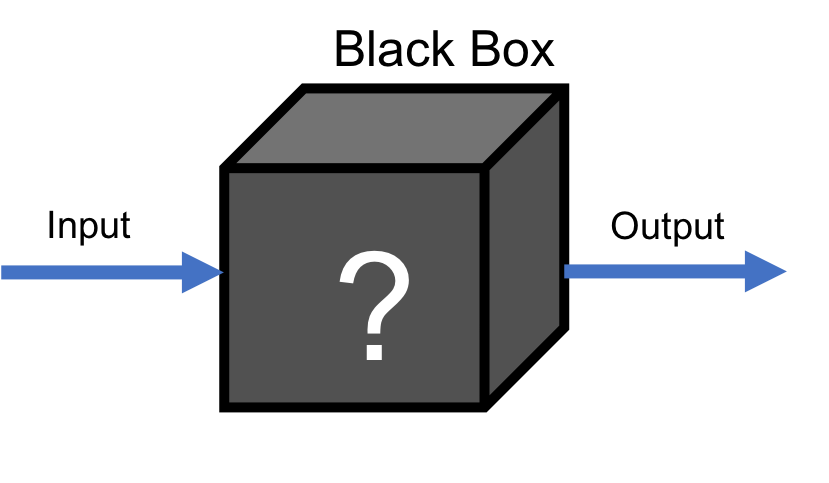
\includegraphics[width=.8\linewidth]{images/black_box.png}
		\label{fig:blackBox}
	\end{subfigure}%
	\begin{subfigure}{.5\textwidth}
		\centering
		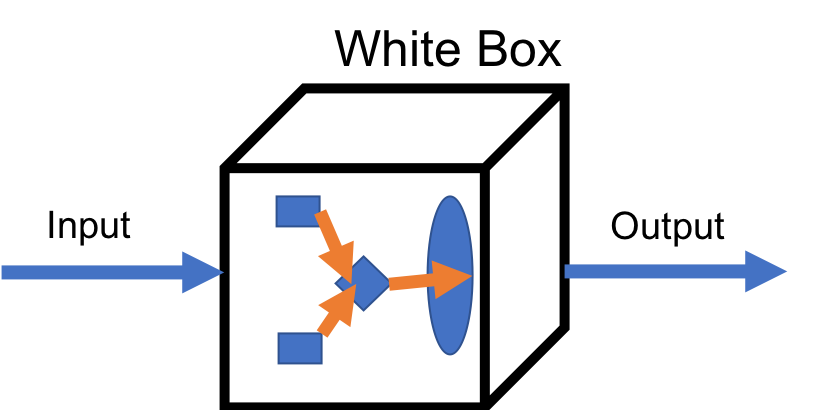
\includegraphics[width=.8\linewidth]{images/white_box.png}
		\label{fig:whiteBox}
	\end{subfigure}
	\caption{A black box scanner derives behaviour strictly from I/O, whilst a white box scanner has all the inner workings of a (web) application at its disposal for analysis}
	\label{fig:test}
\end{figure}


 A white box scanner takes into consideration the implementation of the service, so it may be designed with the specific framework or language used for the application in mind. Conversely, a black box implementation does not care about these details and looks only at outputs from the service. A major differentiation between the two approaches is their use case; a white box scanner emulates the experience of a web developer who is looking to detect potentially exposed parts of his code, whereas a black box scanner portrays the setting for a malicious attacker, where they are only working with the exterior interface of the application to forge an intrusion. The black box approach is the one I will be using in the extension implementation as it aligns best with the project requisites.

\subsection{Automated Vulnerability Scanners}
 
A large majority of web vulnerability scanners are designed to be ran passively. This means an auditor of the security of a web application would start the tool, and depending on the length and intensity of the scan, either grab a coffee while it executes or leave it running overnight. Either way, these are expected to produce reports on where a website is suffering from a vulnerability, which can then be interpreted to produce a fix. This automation is a great bonus because it makes life easier for the auditor, as they can get on with other tasks in the meantime; depending on the initial monetary and time investment needed to set up the scan, doing so automatically can be a cost-effective solution for many businesses. \\

There have been studies committed to evaluate the effectiveness of these black box scanners. Doup\'e, Cova and Vigna did an extensive analysis of the tools available in 2010 \cite{whyJohnnyCantPentest}, including tools ranging from free to \$30,000+ worth. In the same year, Bau, Bursztein, Gupta and Mitchell published their own paper with a similar analysis \cite{stateOfArtAutomatedBlackBoxWebAppVulnTesting}. More recently, in 2015, Parvez, Zavarsky and Khoury released a study on the effectiveness of scanners in detecting a limited set of vulnerabilities \cite{analysisOfEffectivenessOfBlackBoxWebAppScannersStoredSQLStoredXSS}. \\

Doup\'e et al. found that \textit{crawling} was one of the major limiting factors of web vulnerability scanners; according to them, {"...crawling is arguably the most important part of a web application vulnerability scanner; if the scanner’s attack engine is poor, it might miss a vulnerability, but if its crawling engine is poor and cannot reach the vulnerability, then it will surely miss the vulnerability"}. To better understand this, it is important to contextualise what \textit{crawling} is. \\

A typical vulnerability scanner will loosely consist of 3 different modules:

\begin{itemize}
	
	\item \textit{Crawling module} - This is the first part of the scanner that gets executed. A crawler will recursively follow every possible link in a webpage so that the tool can build up an internal representation / database of what the target website looks like. As mentioned above, this stage will make or break the scan - though it is unlikely that a crawler will be able to find 100\% of the available subpages on the target website, any missed links will result in the scanner not considering those pages, which in the worst case scenario may miss a page which is the root of many vulnerabilities on the target site. Acunetix themselves, the providers of the commercial vulnerability scanner, say "if you can't crawl it, you can't scan it!" \cite{acunetixQuoteCrawling}. 
	
	\item \textit{Attacker module} - At this stage, the scanner attempts to chip away at any potential cracks in the website. It goes through every stored entry in the previous phase and scans the content of the associated page. Depending on this content (e.g. a form or a URL parameter), the scanner issues web requests with specially crafted input designed to create \textit{interesting} responses from the web server.
	
	\item \textit{Analysis module} - This module reads the outputs from the target to the attacker module input, and scans for any significant or telling change from the server side response. If the web server generates a wildly different response to a normal input (e.g. it issues a page containing an SQL error message), then this is flagged up as a potential vulnerability. This module can have a feedback loop to the attacker module to refine attack methods. This is done through \textit{fuzzing} - creating mutations of the benign input and testing these on the application until a more malicious input is generated that triggers a vulnerability. The scan completes after all potential mutations and attack vectors have been exhausted, or a resource cap is met (time elapsed, bytes sent etc).
\end{itemize}


\begin{figure}[h]
	\centering
	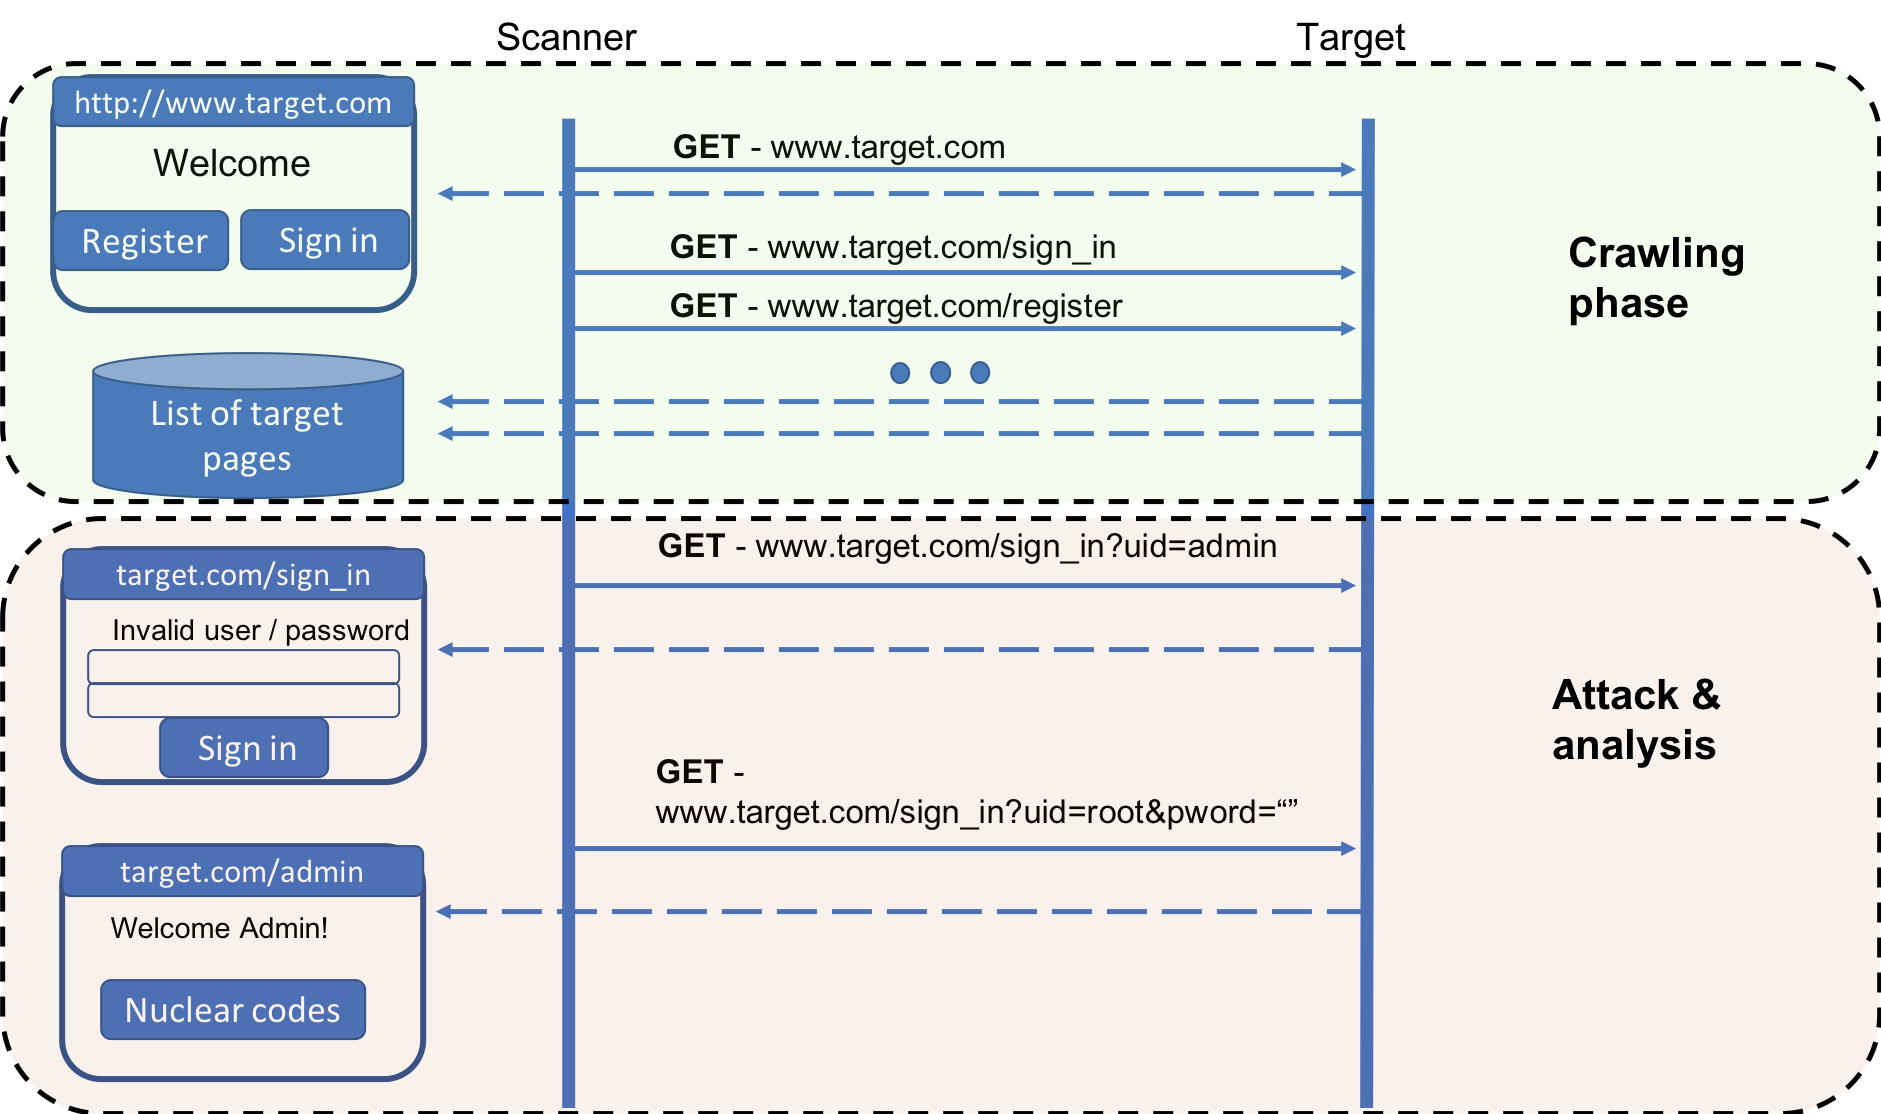
\includegraphics[width=\textwidth]{images/scanner_structure.png}
	\caption{The typical structure of a vulnerability scanner. The crawling phase builds up a database of potential pages to attack. During attack, malicious inputs are fired towards pages to try and trigger undesired behaviour - the analyser reads response contents with some heuristics to determine what responses seem to indicate vulnerabilities.}
	\label{fig:test}
\end{figure}

With this knowledge in mind, it is now easier to appreciate how important the crawling phase is, as it sets an upper bound to how far a scanner can go. Crawling in itself is however not a trivial task to implement. A naive approach to this would be to start at the target page given, scan for any \texttt{<a>} anchor links in this page and filter this list to only include links that belong to the target domain (e.g. if our target was \texttt{facebook.com}, we might be interested in \texttt{facebook.com/account}, but we would discard any links to \texttt{google.com}, as Google links belong to a different domain. As a general rule of thumb, the links we explore have the target link as a prefix to the URL). This method of crawling pages would quickly come up against issues though. A lot of the interesting state of a web application is often hidden behind a login form, so if a valid user account isn't created then a scanner will not be able to explore the full array of actions available. The method described above would not consider this, so would skip out on all the intriguing parts of a website that requires you to have an account. There are also other technologies used in the web that make this slightly harder, such as Flash objects that contain useful sublinks. These objects are not straightforward to analyse, and make automated crawling difficult. \\

This combination of components quickly complicates things for creation of an effective crawler implementation. A competent crawler needs to go above and beyond being just a database of pages - it has to emulate human interactions with an application without any prior domain knowledge. To do so, it has to somehow derive an internal representation of what the website looks like, and refer to this state when crawling and in the analysis phase. Keeping state was an issue raised by Doup\'e et al. in \cite{whyJohnnyCantPentest}. As an example of its importance, if during the attacking phase the scanner is logged in, and an attack request causes the scanner to log out of the application, all the subsequent requests will execute in a different context where the scanner is logged out, invalidating their intended purpose. Doup\'e, Cavedon, Kruegel and Vigna later addressed this by creating a scanner that generated an internal state machine representation of a web application based on heuristically unique server responses \cite{stateAwareBlackBoxWebVulnScanner}. The techniques demonstrated in that paper were useful in creating a more effective crawler that remembered state so as to not waste computation efforts. The resulting scanner achieved higher code coverage rates for web applications analysed over other otherwise similar, open-source scanners. Higher code coverage rates mean that a scanner is exercising more of the application's source code, thus increasing likelihoods of finding a vulnerability. \\

It is clear that an automated crawler based web vulnerability scanner is a difficult tool to create. The shotgun approach used by the crawler can also have negative consequences for the application as discussed in \ref{ethics}. Though state of the art crawlers can now handle the aforementioned hurdles and other intricacies of different web applications, the creation of an efficient, fully automated crawler could warrant a project of its own. \\

 
\section{Browser extensions} \label{browserExtensions}

I propose to create the tool described as a browser extension in Google Chrome. An extension seems to be ideal as a method to accomplish the intended functionality for 2 main reasons.

\begin{itemize}
	\item \emph{Extension privileges} - A browser extension works as a self-contained application that is trusted enough to expand the browser experience. Chrome predefines a potential permission set an extension can tap into. Each extension must declare which of these it will be using in a \texttt{manifest.json} file, as well as list of which domains it expects to be ran on. Upon installing the extension, the user is asked whether they wish to allow this behaviour. As required by the project, an extension can contact remote servers (allowing it to replay user actions on their behalf), as long as the appropriate cross origin permissions are appropriately set up.
	If an extension is compromised, the application of the least privilege principle can mitigate potential damages because it will only be able to possibly affect the declared domains at the previously granted permission level. It is therefore good practice to declare the minimum amount of domains and permissions required to get the extension to work. 
	
	An extension has a \texttt{background.html}, a page which runs invisibly as the user browses. This is where most of the logic and state of the extension is stored, but it cannot directly interact with target pages. For this, there are \textit{content scripts}; these are small Javascript programs that are injected into the selected domains and can interact with the Document Object Model (DOM) of a website and modify it according to the programmed needs. It is important for extension behaviour to not break functionality of existing sites. For example, if a web application is using JQuery 1.0 and the extension is using JQuery 2.0, it would be unacceptable for the newer dependency on the library to break the existing functionality, so content scripts are isolated from the existing page scripts. This is done through \emph{isolated worlds}, which create a sandboxed copy of the website DOM to avoid clashing between content and scripts and existing scripts. Because the content script can interact only with the website, it may be desirable to establish communication with the extension core to send information back to the \texttt{background.html} to process. For this reason, there exists a message listening API between the \texttt{background.html} and the content script to allow communication. 
	
	It is important to keep these separate for security reasons. If a content script is compromised by a malicious page targeting the extension, the attacker still has to exploit another vulnerability in the background page to exfiltrate any data. Additionally, the entire extension itself runs in a separate process to the browser and other extensions. This means if an extension is compromised and begins to degrade the system, this process can simply be halted without killing the browser or other innocent extensions.
	
	Additionally, extensions run on HTML5, CSS3 and support Javascript running on Chrome's own engine, with native JSON capabilities. They support the latest web technologies and as such are not heavily restricted on the use of these, as other methods used in black box scanners are. Therefore, browser extensions run at the appropriate level of abstraction to perform the necessary technical operations without much hinderance. 
	
	\begin{figure}[h]
		\centering
		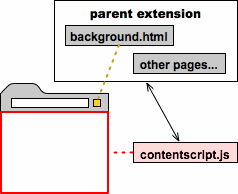
\includegraphics[width=0.4\textwidth]{images/extension_arch.png}
		\caption{An extension is split into 2 main areas. The \texttt{background.html} page has access to all extension privileges and is where the business logic of the extension is stored. It cannot interact with user webpages. Content scripts can be injected to interact with the DOM of a page. The \texttt{background.html} can contact the content script via a message passing API. Image courtesy of Google Developer documentation. \cite{chromeExtensionArchitecture}}
		\label{fig:test}
	\end{figure}
	
	\item \emph{User operability} - Because of the features described above, the extension can be designed in such a way that allows it to sit between the user and the web application and seamlessly create the desired semi-automated experience. Wherever possible, depending on the type of vulnerability, it would be ideal to give the user interactive visual cues for when the scan has detected something that merits further research. If the vulnerability is attached to a specific form that takes user input for example, the extension should have the capabilities of identifying the DOM object for this, and add a small tooltip around the visual area of this object to initiate the deeper scan analysis. If the vulnerability is not necessarily caused by visible means, then the extension is also able to create other appropriate visual cues, such as a fixed position element. 
	Being able to implement these characteristics should result in a more intuitive user experience. 
	
	This also means that the user will not be doing any heavy lifting - the extension will be passively searching for vulnerabilities as they use the website, but should also be able to be activated at user will. During the phase where the tool begins to replicate user actions to investigate a vulnerability (explained further in \ref{contribution}), if implemented appropriately, the extension will be able to repeat the human steps of submission and navigation at a much faster rate than a human would do, with several more inputs.
	
\end{itemize} 

\chapter{Design}


\section{Project Contribution}
\label{contribution}

These points lead us nicely onto the intended innovation behind the project idea - to create a semi-automated web application vulnerability scanner. The essential difference between this and the aforementioned black box scanners is that it intends to work as an aide alongside a pentester, not as a fully automated background process. \\

The proposition of creating a tool that is driven by user input seems appealing for a number of reasons:

\begin{itemize}
	\item \textbf{Full Experience} - A scanner that analyses a web application for vulnerabilities as a user is using the application has fewer limitations as to what is within its scope. As pointed out by \cite{whyJohnnyCantPentest}, scanners struggle to scour through more complex constructs of the internet such as convoluted Javascript forms, AJAX requests and Flash objects. As a result, many scanners ignore these features altogether, dismissing potential vulnerabilities in the process. A user driven experience allows the user to interact as they would normally with these technologies, and can analyse inputs and outputs accordingly.
	
	\item \textbf{Educational} - As mentioned above, one of the issues that leads to the need of vulnerability scanners is the lack of security-aware developers. By developing a tool that works alongside developers, they can refine their skills in this area if they already know some security basics. There is also room for learning for website owners as penetration testers may demonstrate the severity of exploits caused by vulnerabilities using the tool, and mitigating these. 
	
	\item \textbf{Simpler crawling module} - Since the tool is not scouring the entire site at once but is rather following the more natural workflow of a human user, the equivalent crawling module will only need to keep a much smaller representation of the website as opposed to before. A proposed methodology to simplify this process given the project specification is to create a crawler based on recommendations and an 'action replay' mechanism. 
	
	The recommendation algorithm will need to be based off of similar existing algorithms in automatic crawlers. Since the tool must be driven by user input, the crawler would analyse contents and interactions of the web application with the user (as it would do automatically), and suggest specific features to the user as a starting point for the scan. This can be done by passively reading the contents of web requests between the user and the web application and flagging up any that seem to exhibit behaviour of an insecure system, such as passing user inputs in clear text, or using client-side inputs to control important application sensitive logic. Once a user chooses to follow a recommendation, they may investigate the flagged feature more closely.
	
	At this point, the 'action replay' algorithm begins - once a user has elected a potential target to test for a vulnerability, the tool begins to record user actions. Depending on the selected feature and what vulnerabilities may be discoverable, the tool can then suggest a stopping point of recording, or wait for the user to determine when their actions that detect a vulnerability are enough. The tool then takes these actions and analyses their outputs - it may be the case that a user has found a vulnerability on their first go. It could also be the case that this input didn't trigger a vulnerability, but is worth looking into further. At this point, the crawler will begin to fuzz different versions of input that may be more effective at showcasing vulnerabilities. In recent research by Parvez et al. into evaluating black box scanners \cite{analysisOfEffectivenessOfBlackBoxWebAppScannersStoredSQLStoredXSS}, one of the final recommendations for a better scanner was to add interactive multistep options to the scanner, which is a main focus of this method. To the best of my knowledge, this 'action replay' algorithm is a novel approach in this area.
	
	\begin{figure}[h]
		\centering
		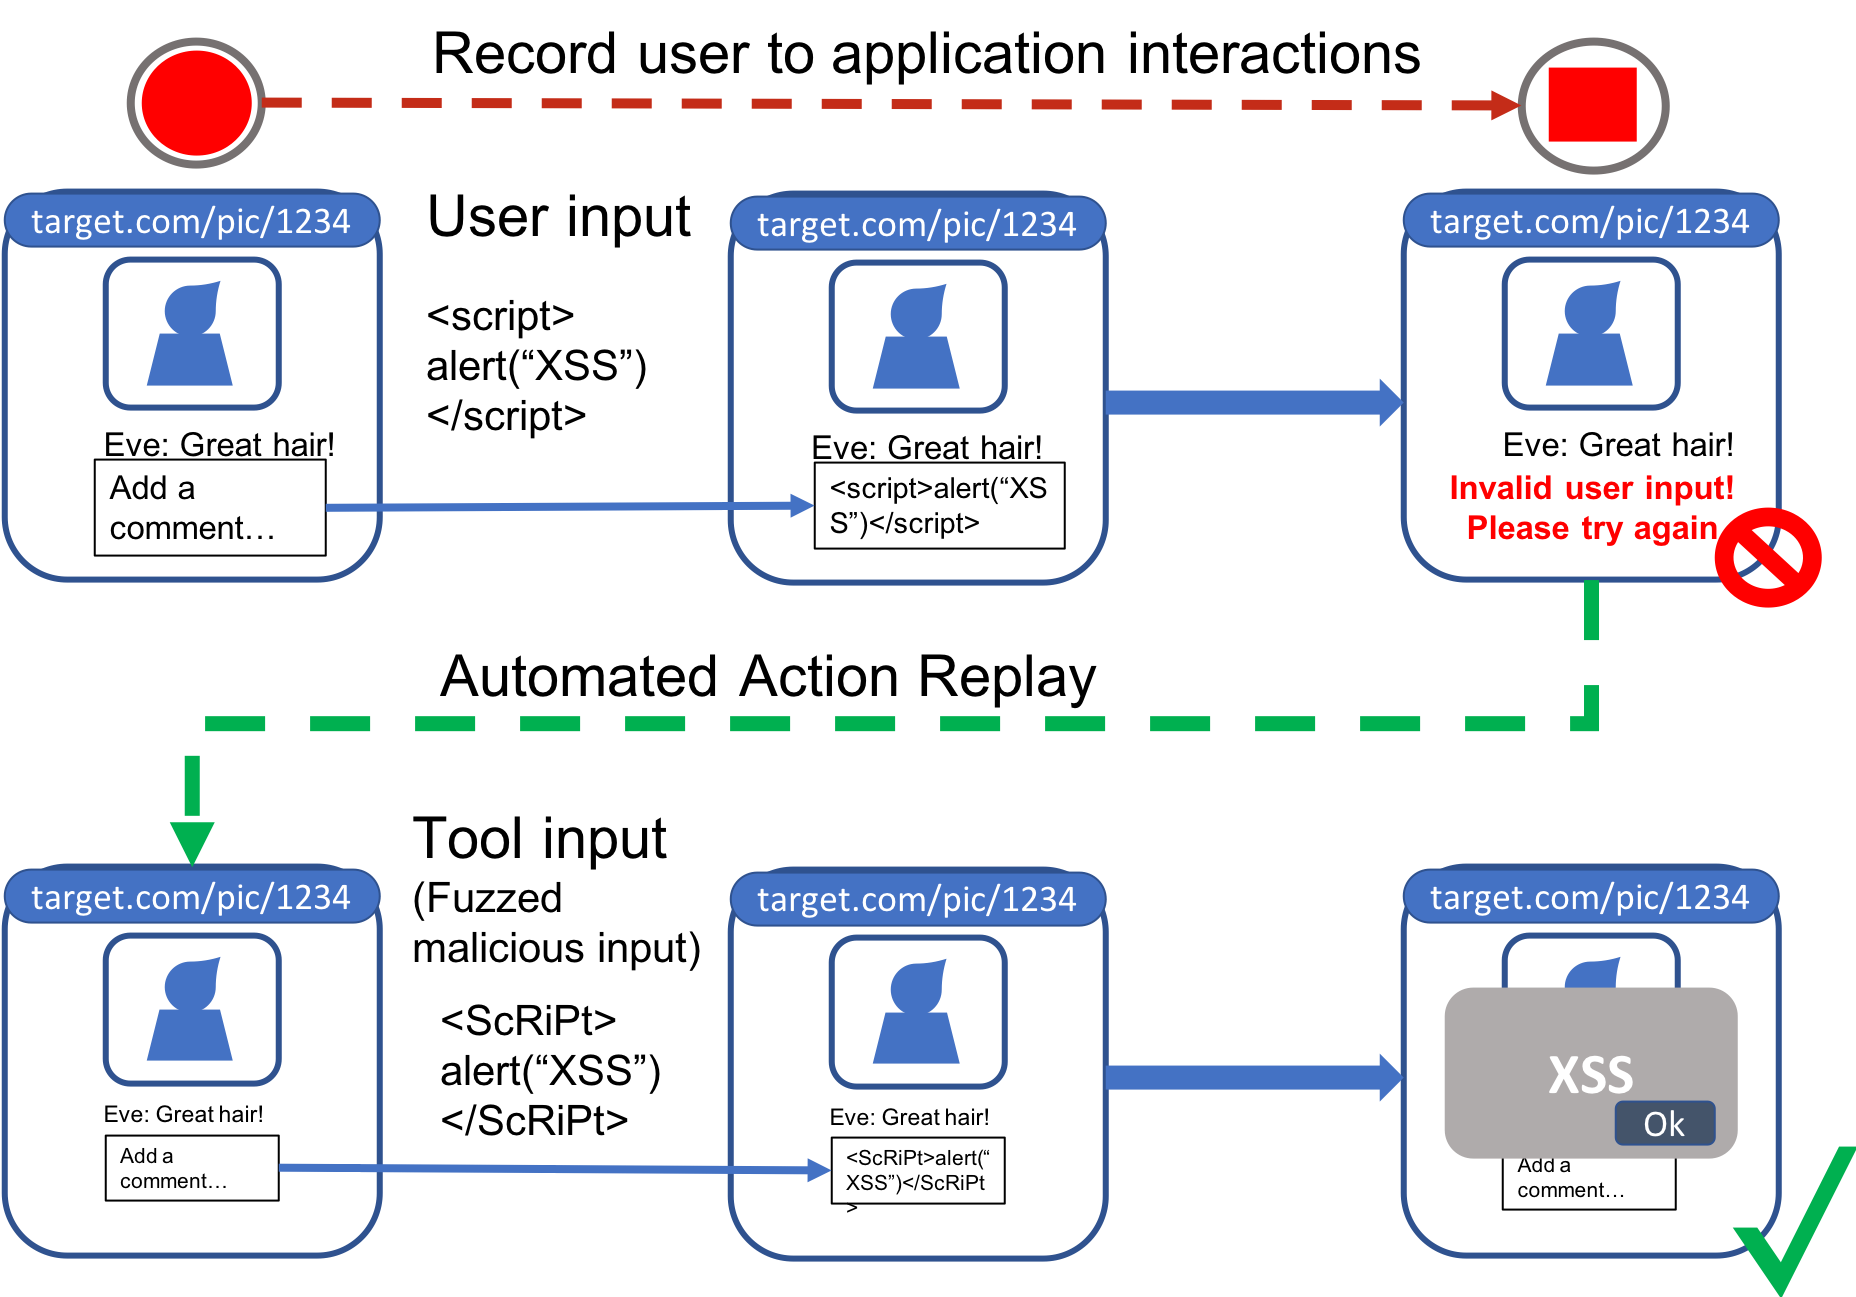
\includegraphics[width=\textwidth]{images/action_replay.png}
		\caption{A visualization of the proposed action replay algorithm. The tool records user input for a time period determined by the user. The tool then replicates actions using fuzzed inputs to try and uncover vulnerabilities if the first attempt was unsuccessful.}
		\label{fig:test}
	\end{figure}
	
	
	\item \textbf{Human judgement} - The previously mentioned paper by Parvez et al. also mentions that choosing the right attack vectors to exploit vulnerabilities is still a big challenge for black box scanners \cite{analysisOfEffectivenessOfBlackBoxWebAppScannersStoredSQLStoredXSS}. Huang et al. recently built a scanner that performed well against open-source competition \cite{webAppSecThreatsCountermeasuresPitfalls}. However, these authors recently acknowledge that \emph{"there is no silver bullet for web application security; threats will continue to grow and evolve"}. Herein lies much of the motivation for making this project user-centric: vulnerability detection and even exploitation may be automated \cite{darpaAIChallenge}, but for now, efforts in having to build an AI that is able to do this are astronomical - it takes years for teams of experts to build tools that do this. Following its recent success, the winner of the DARPA Cyber Grand Challenge (an AI-only capture the flag contest) was pitted against human professionals at the 2016 DEF CON CTF Challenge, where it came last \cite{defcon16Results}. These efforts show a bright future for fully automated security systems, but these may still be some years away in the full making. This project does not admit defeat in attempting to automate the process of countering malicious agents, but rather aims to increase the likelihood of doing a good job against them by covering our bases with higher quality base defences. In fact, even limited domain knowledge has shown to be useful for human penetration testers; a group of students with 'average' security skills achieved a higher success rate on their own than some vulnerability scanners in analysing web applications \cite{whyJohnnyCantPentest}. It is hoped that with the correct suggestions provided by the tool, this project lowers the minimum requirements of a successful user to be 'below average' in their security domain knowledge. \\
	
\end{itemize}



\section{Limitations}
\label{limitations}

In order to be able to effectively evaluate this project at a later point, it is important to delineate realistic expectations in terms of what it can and cannot do. 

\subsection{Time taken}
Since the extension is user driven and not fully automatic, the suggested process will be inevitably slower than if it was otherwise automated - there will be waiting times as users will not instantly attempt to uncover recommended vulnerabilities. There may also be some intellectual effort involved in crafting initial input to try and do this, which adds to this. Both of these factors add to 2 different metrics: the total scan time and the time taken from recommendation to decision of whether a vulnerability is found or not. \\

Total scan time may be especially hard to measure, and can be seen as a disadvantage of this scan. It is not known whether a user will eventually go through every possible page that is relevant, so it becomes very difficult to claim an end to the scan. On the contrary, automated crawlers \emph{will eventually} come to an end their search, and thus put an upper bound on how many resources they can analyse. Human driven crawling may stop or resume at any given point. Not being able to best assess the total scan time is an acceptable tradeoff of this project as it will simply not be avoidable given human driven interaction is being explored. \\

The time taken to ascertain whether a vulnerability exists or not from a recommendation can however be bounded. This period begins when a user decides to investigate a recommendation on their own or by suggestion of the tool, and finishes either when enough proof of a vulnerability has been observed, or when all possible fuzzing opportunities in exploiting it have been exhausted - the extension will have a list of possible fuzzing mutations per type of vulnerability, so this work is bounded by that list. Again, since this is not a fully automated tool, the extension is expected to take longer in this metric due to human interaction when comparing it to automated scanners, which is only natural. \\

\subsection{Breadth of  work}
Section \ref{vulnerabilities} describes many potential kinds of vulnerabilities that the project may choose to tackle. Some of these are harder to detect than others, and thus require more development work. This large scope may make it tempting to try and undertake too many things at once. At the time of writing, it is also hard to assess just how difficult it may be to implement scanning for a specific type of vulnerability. The extension will be developed with aims of finding revelant vulnerabilities - sorted by both volume of occurrence and contemporary relevance as found on surveys. One of the most recurring vulnerabilities in both aspects is Cross Site Scripting, so developing the tool to be able to detect this class of weaknesses is a good starting point. Other features that may seem small (such as analysing cookies or the use of iFrames on a page), may also be beneficial to implement. As the project develops, it becomes harder to weigh the costs of effort to implement versus the success rate of focusing on a specific feature, so some further time should be allocated to allow for this meta research. \\ 

\subsection{Self security}
The security of the extension being developed should not be taken for granted. As mentioned above, Google Chrome has several mechanisms in place to safeguard extensions from falling prey to malicious attackers. Namely, these are:
\begin{itemize}
	\item \textit{Isolated Worlds}
	\item Privilege separation
	\item Predefined permissions
	\item CSP (Content Security Policy)
\end{itemize} 
Although these practices make it much easier for a developer to avoid serious mistakes, it is still possible to write vulnerable extensions. The \textit{threat model} in this case (the way we choose to archetype our potential enemy), is by means of a web attacker. This would be someone who sets up a 'honeypot' website, expecting the extension to scan it but in the process attempt to compromise the extension by different means. Due to the priveleges granted to an extension, this may result in the jeopardizing of sensitive user data, such as their passwords. A recent paper by Carlini, Felt and Wagner reinforces the notion that Chrome's existing techniques are effective in preventing extension compromise, but also list some developer practices that could result in vulnerabilities, such as the unrestricted use of the \texttt{eval} function by Javascript (which is known to be dangerous as it executes given strings as commands), and injecting website data into HTML \cite{evalChromeExtensionSecurityArchitecture}. Many of the notions mentioned in the paper are also cited in Google's own documentation on how to write Chrome extensions \cite{chromeExtensionArchitecture}. Following these best practices will decrease potential risks associated with this project. \\ 

\subsection{Ethics \& Handling of Results}
\label{ethics}
This project aims to build a tool that helps users find vulnerabilities in web applications. Obviously, this may raise ethical ramifications as to how the tool interacts with websites, and how its output is handled. \\

As the tool needs to send requests on the user behalf when executing (especially so during the 'action replay' phase described above), the rate at which this is done may be of concern. Conventional automated scanners may fire 100's of different fuzz attempts at a web application, \emph{per vulnerability, per existing page} - a shotgun-like approach. This approach is very intensive, and for web applications set up for smaller amounts of traffic, may result in a Denial of Service (DoS). This tool aims to reduce this by only passively reading user crawled content, and only actively interacting with the website whenever a flagged vulnerability has been detected. \\

A related concern is to do with the scope of testing and uses on a real web application. For testing and evaluation purposes, the tool will be ran against existing, known to be vulnerable applications, such as DVWA \cite{dvwaSite}. Ideally, it should also be ran against other web applications beyond my control. However, for some of these, it may be the case that running the unhinged extension may infringe usage terms and agreements. For this purpose, a proposed restrained mode for the tool may be built, such that it does not actively take any action when browsing web applications, but rather only passively reads network traffic to deduce and recommend potential vulnerabilities. \\

Naturally, as per the project ideals, any vulnerabilities that may be found as a result of running this extension will duly be reported to the appropriate developers.
\chapter{Implementation}


%5\section{Extension Structure}

As explained in \ref{browserExtensions}, the extension is split into different files for both security reasons and other separation of concerns.
The diagram below puts into more detail the exact structure of the extension in context with some of the real files being used.


\begin{figure}[h]
	\centering
	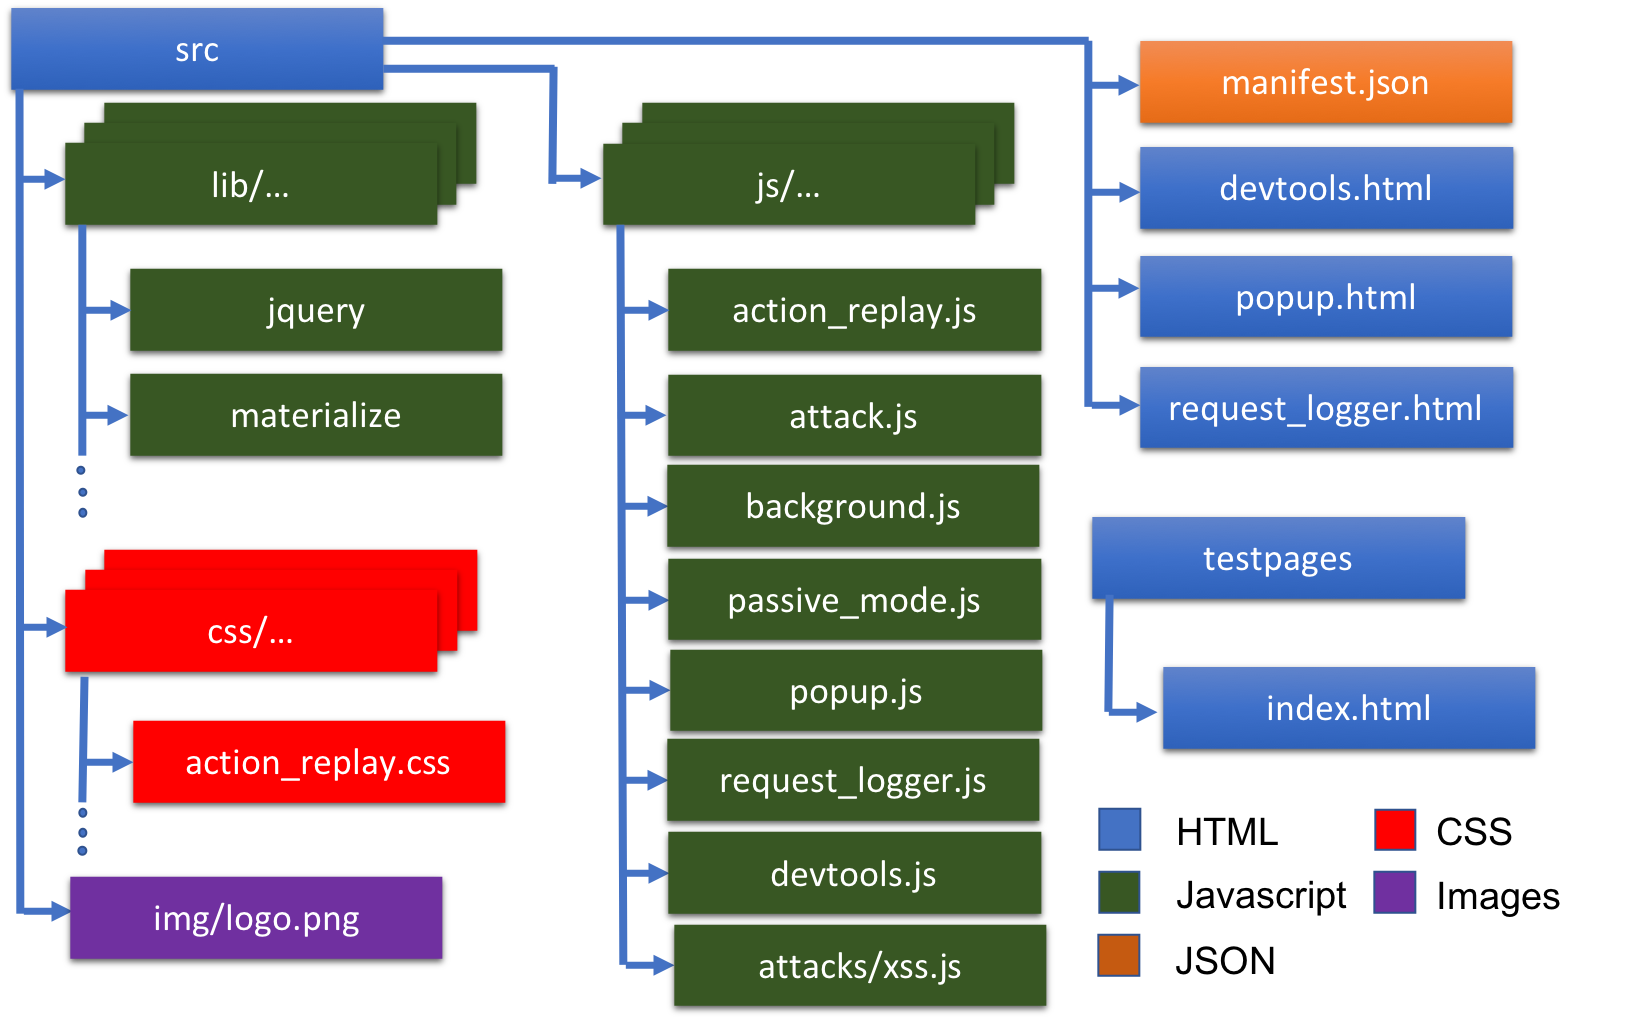
\includegraphics[width=0.9\textwidth]{images/project_structure.png}
	\caption{The directory structure used for the project}
	\label{fig:test}
\end{figure}

I have arranged the files in question into 2 separate subfolders - the \texttt{testpages} directory keeps the source code for the test harness page with vulnerabilities, while the \texttt{src} directory keeps all the other extension related code. \\

Within \texttt{src} we find different folders for separate concerns - \texttt{lib} stores any library code I have imported from a third-party, \texttt{css} keeps custom styles used across the extension, \texttt{img} is where any images are kept, \texttt{js} holds any custom produced Javascript files, and is where most of the logic within the extension lives. \texttt{src} also contains the \textit{manifest} file, and any HTML page code. 

\section{Manifest}

The manifest is where the extension declares its intentions by enumerating all the scripts and files to be accessed, as well as the permissions required to run the extension as an add-on to the browser. This file is necessary due to security reasons; each extension is expected to run as a standalone program within the browser. Any dependencies are to be declared and included within the package before the program is run, with the exception of contents that are whitelisted in the declared \textit{Content Security Policy} (CSP) directive within the file. I am using the recommended default CSP directive of \texttt{script-src 'self'; object-src 'self'}. This policy actively prevents notoriously dangerous Javascript functions from being evaluated, disables in-line Javascript functionality (which enforces a separation of content from behaviour), and, as the name suggests, will only load scripts and files locally available to the package \cite{chromeExtensionCSP}. \\ 

A potential methodology to use in a setting like this would be to employ a bundler to create a single minified (or compressed) \texttt{.js} file that includes all the required libraries and code to be imported. An example of this is  \textit{Webpack} \footnote{\url{https://webpack.js.org/}} - I did not employ a bundler like this as I learned about its uses later into the project. Furthermore, I am including a relatively small number of third-party sourced code, making this a small practical concern. \\

Other noteworthy details from the manifest file include:

\begin{itemize}
	\item The \texttt{devtools\_page} directive - this is necessary to access the developer tools API's within the extension, which provide extra information when using the extension such as the contents of the requests sent at any given time. See \ref{devtools}.
	
	\item The \texttt{web\_accessible\_resources} directive allows me to specify resources which should be accessible in the context of a normal browsing experience. This is a feature enabled in the more recent 2.0 version of the manifest, which blocks resources by default unless they are whitelisted in this manner. This prevents malicious attacks on the extension, such as fingerprinting or exploiting XSS vulnerabilities \cite{chromeExtensionWebAccessibleResources}. An example of a resource included here is the \texttt{request\_logger.html} page.
	
	\item The \texttt{content\_scripts} to be included in every page are also defined here - this includes both CSS files as well as third-party libraries and Javascript vulnerability scanning files.
\end{itemize}

\section{Test harness}

In order to be able to appropriately test for features in development for this extension it is necessary to have access to a fragile website. It would not be ethical to use a website in production to test my extension against; doing so could result in all manner of adversities for the owner of that web address. That is under the assumption that I could firstly find a fragile website to test against; despite the prevalence of security weaknesses spread through the web, it is inherently a difficult task to identify and exploit these. Therefore, I have developed a deliberately weak website to test against. As will be demonstrated in each of the following sections, this harness website (stored under \texttt{testpages/index.html}) can be used to showcase an example of each vulnerability and consequent attack. \\

In order to emulate the website as a server, I am using the out-of-the-box implementation of Python's \texttt{SimpleHTTPServer}. To run this, I simply have to run \texttt{python3 -m http.server 8000} to start a server on the localhost at port 8000. This allows me to submit forms and thus emulate query parameter submissions.

\section{Popup page}

This is the main interaction point for a user utilizing the extension. The layout of this page makes a clear distinction between the different features available to use in the extension. \\

\begin{figure}[h!]
	\centering
	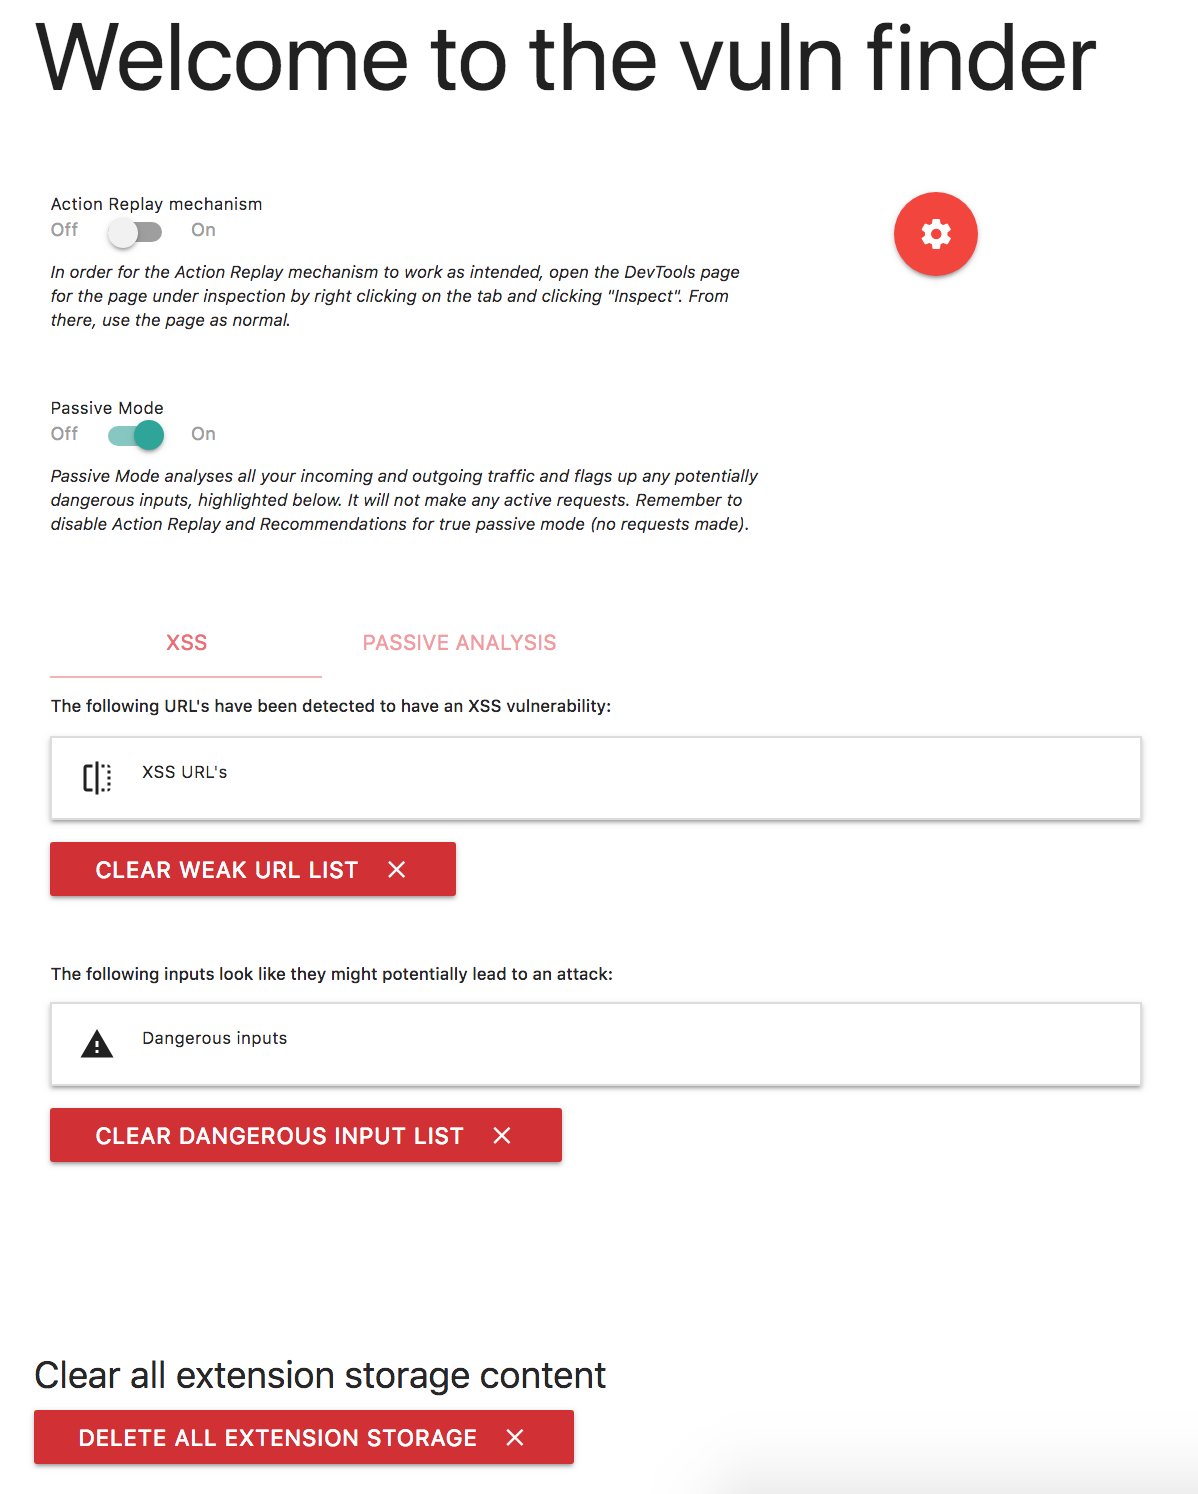
\includegraphics[width=0.8\textwidth]{images/popup_full.png}
	\caption{The main contents of the popup page when first clicked by a userw}
	\label{fig:test}
\end{figure}

This page offers an accessible means for tweaking and toggling all the options available in the extension, as well as viewing and analysing the outputs from the different modes of running the extension.  


\section{Background Page}

The background page I am using in the extension is a persistent page, meaning it is constantly running. This is in contrast to event background pages, which are opened and closed as necessary depending on the occasion. I am using this page to listen for messages sent from other scripts to be able to set aesthetic updates, as well as establishing a connection with the \texttt{devtools} page to subscribe to and forward custom request messages to content scripts.

\section{Request Logger}

This page is designed to capture information from attacks that have successfully hijacked Javascript execution and diverted a user to this page. In order to be accessible from any other window, it must be declared as a \texttt{web\_accessible\_resource}. It captures the page it was referred from and reports it as a page where a vulnerability exists.

\section{Devtools} \label{devtools}

The devtools page has access to a specific set of API's designed to extend the experience for web developers using the browser. This includes access to the currently inspected window, the developer panels, and network request information \cite{chromeExtensionDevTools}. \\

\begin{figure}[h]
	\centering
	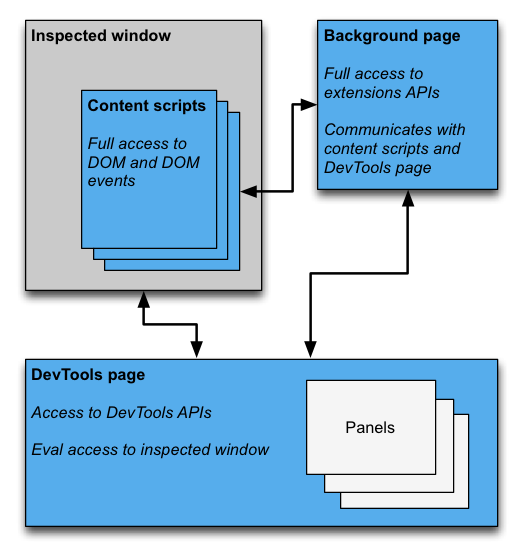
\includegraphics[width=0.55\textwidth]{images/devtools-extension.png}
	\caption{An extension making use of the DevTools API's further extends the capabilities of a standard Chrome Extension. Diagram from \cite{chromeExtensionDevTools}}
	\label{fig:test}
\end{figure}

More specifically, I am interested in the \texttt{devtools.network} API - this provides access to every request once it has finished. This contains a wealth of information which is otherwise difficult to obtain without using the devtools API. One of the APIs I am also using in the extension is the \texttt{chrome.webRequest}. This gives me access to several different events at different points of the lifetime of the request. It allows me to access some headers as well as change a limited set of these. It however does not provide sufficient information for the purposes of the extension - \texttt{devtools.network} gives access to the response content of any given request, which is vital in analysing outputs from a request to create attack correlations. Accessing the \texttt{devtools} APIs requires the Developer tools to be open for the page in question, which is only a small inconvenience when using the extension.

\section{Message Design}

To better understand the structure of the extension and how each feature ahead is to be implemented, it's good to create a high level overview of messaging between each component.  \\

\begin{figure}[h]
	\centering
	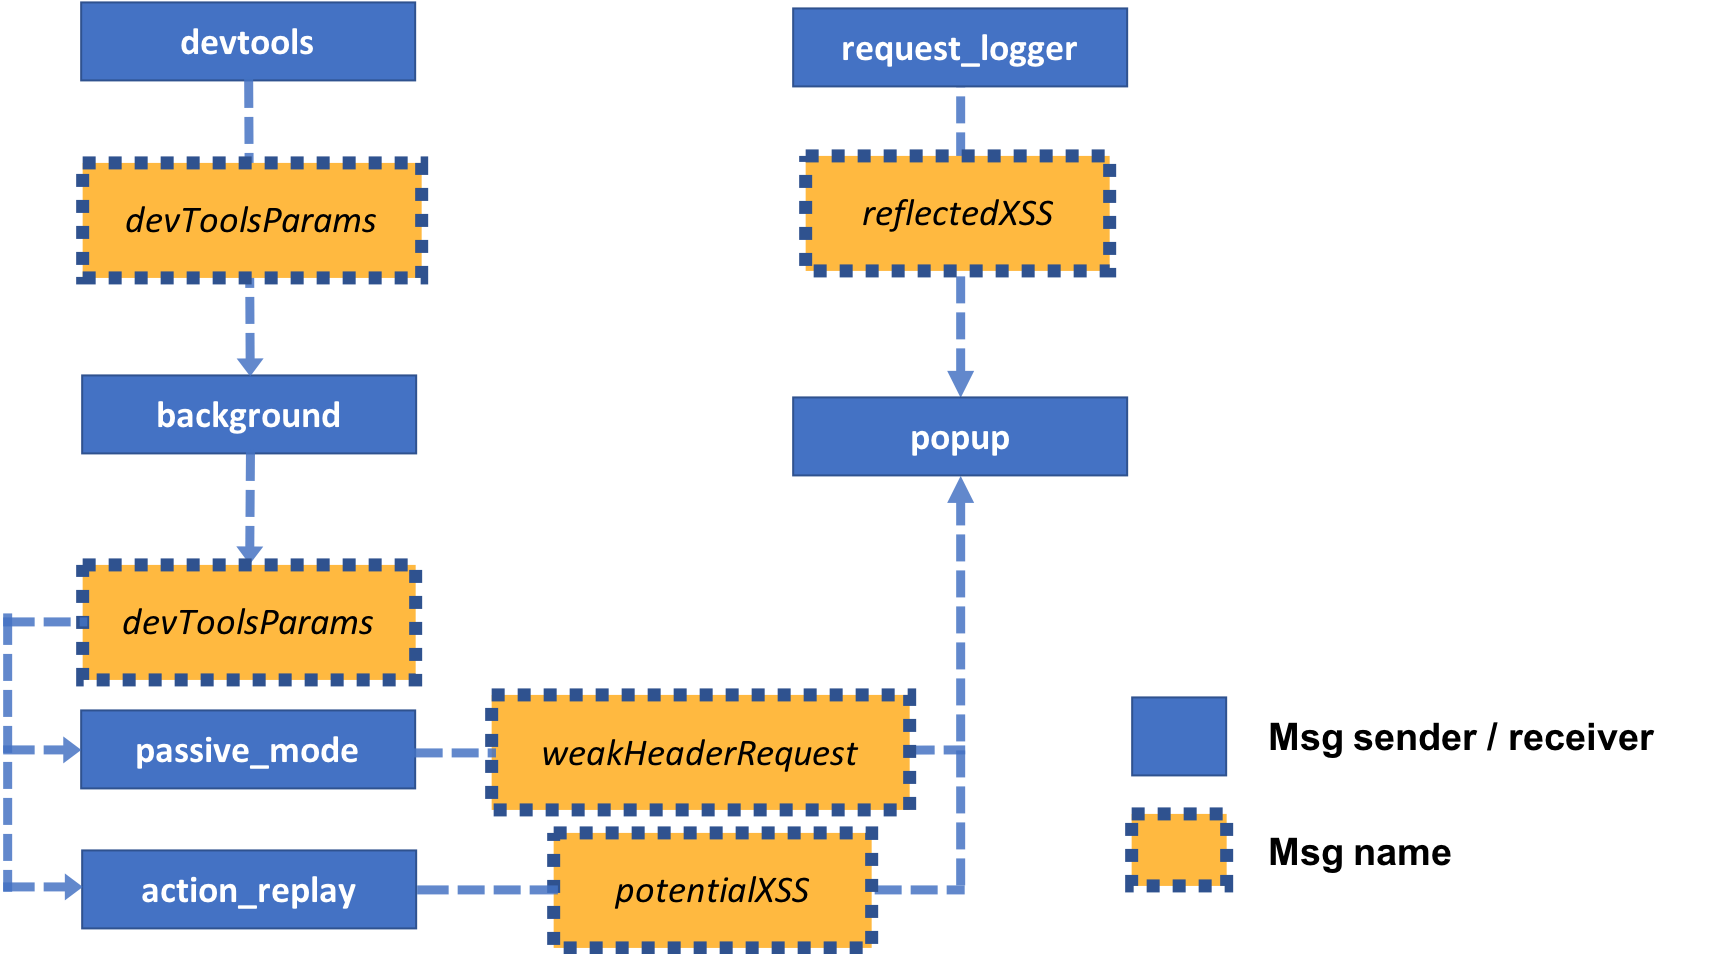
\includegraphics[width=0.95\textwidth]{images/message_passing.png}
	\caption{This diagram illustrates the passing of messages within the different components in the extension}
	\label{fig:test}
\end{figure}

In order to analyse the requests being made in different context scripts, the \texttt{devtools} script gathers every request made in the page which has the Developer Tools inspection windows open. Since this page cannot directly pass messages to the content scripts \cite{chromeExtensionDevTools}, it uses the background page as a mediator. It establishes a connection to the background page and passes to it every request it picks up. The background page then forwards these messages to the different content scripts that analyse the requests - \texttt{action\_replay} and \texttt{passive\_mode}. \\

Whenever a request causes the \texttt{request\_logger} page to be loaded, the page captures the information from the page it has just been referred to from, and forwards this information in a message to the \texttt{popup} page to update the list of vulnerable URLs. To toggle the enabling or disabling of the Action Replay algorithm, the popup page sends a message to the \texttt{action\_replay} script each time the corresponding switch is clicked. When the Action Replay is mid analysis, it will produce a warning list of inputs it has considered to be potentially dangerous, and passes a message to the \texttt{popup} page when it has detected this. Similarly, in the \texttt{passive\_mode} script, a message is passed to the \texttt{popup} alerting to any suspicious request behaviour. The \texttt{background} script also listens to several of these messages, and consequently updates the UI badge aesthetics, alerting the user to fresh information to analyse in the extension.

\section{Chrome Storage} \label{storageSpecs}

Google offers access to the \texttt{chrome.storage} API, which is a specialised storage designed for the needs and uses of an extension. This is an asynchronous storage that allows storing of objects (not solely strings as is found in \texttt{localStorage}). Perhaps most practically, it also allows each content script to access storage data without the need to relay this information through the background page. At the start of the project I was using \texttt{localStorage}, but quickly switched to \texttt{chrome.storage} once I ran into the hassles of using this (converting to and from a \textit{string} type on access and storage, as well as using the \texttt{background} as a proxy for every access). \\

I am using this storage to keep a variety of settings and flags, as well as different lists of requests and analysis. Namely: 

\begin{itemize}
	\item \texttt{passiveModeRequests} - This collects all the requests gathered when running the Passive Mode in the extension. This stores request and response params, headers and cookies, as well as the response content and the URL pertinent to the request.
	
	\item \texttt{passiveModeWeakHeaderRequests} - Initially intended to store the requests which have been detected to have weak security Headers, this stores an array of requests with properties similar to the \texttt{passiveModeRequests}. The difference between what is stored is that in this array I also store a list of warnings added to the request by the passive mode if it has found any worrying information during its scan.
	
	\item \texttt{settings} - This is an array of flag settings determined in the settings section of the extension. It stores information such as the \texttt{recommenderSensitivity}, \texttt{passiveModeCSRFEnabled} and \texttt{passiveModeWindowSize}.
	
	\item \texttt{cachedSettings} - This stores the same information as \texttt{settings}; \texttt{cachedSettings} are used to store settings before these are saved in the settings window.
	
	\item \texttt{potentialXSS} - This stores a list of user controlled inputs involved in XSS detection. Each input stores its type - \textbf{cookie}, query \textbf{param}eter or \textbf{header}. The input also stores the URL of origin, and the name and corresponding value of each value in consideration.
	
	\item \texttt{ARrequests} - This list stores every request that is captured within the currently / last recorded session of the Action Replay algorithm. The information kept per request is similar to that kept in \texttt{passiveModeRequests}.
	
	\item \texttt{ARSession} - This flag keeps track of whether the current Action Replay session is recording or stopped.
	
	\item \texttt{enableAR} - Enables or disables Action Replay in the current page.
	
	\item \texttt{enablePassiveMode} - Enables or disables Passive Mode in the current page.
	
\end{itemize}

\section{Recommendations} \label{recommendations}

One of the large features intended for implementation in this project was the use of suggestions whilst browsing a page to attempt vulnerability exploits. This provides a low-effort means for a penetration tester to quickly test different types of attacks on a webpage. \\

The recommendations in the extension work by analysing the contents of the page, and tweaking the page accordingly. It begins by reviewing every \texttt{form} tag in the page - for each form found in the page, it will detect any child \texttt{input} tags, and for the first of these will create a sibling node which acts as a prompt to analyse the page further. \\

The sibling node with the text \textit{Investigate form} is made into a clickable element, and upon click will initiate an attack attempt against the input in question. 

\begin{figure}[h]
	\centering
	\begin{subfigure}{.5\textwidth}
		\centering
		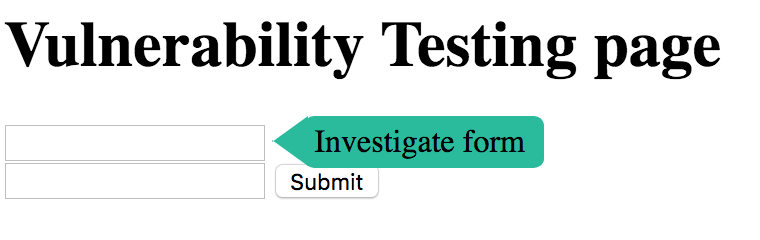
\includegraphics[width=.8\linewidth]{images/test_page_investigate_form.png}
		\label{fig:test_page_investigate_form}
	\end{subfigure}%
	\begin{subfigure}{.5\textwidth}
		\centering
		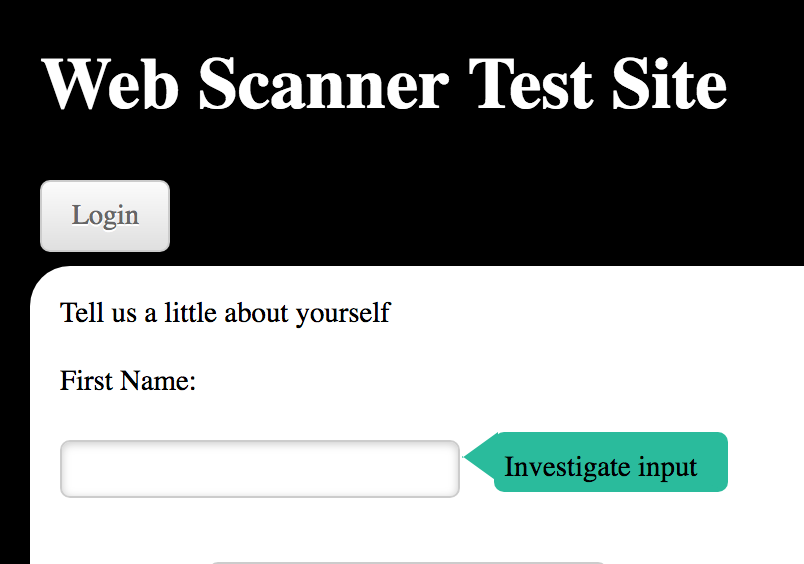
\includegraphics[width=.8\linewidth]{images/web_scanner_investigate_form.png}
		\label{fig:whiteBox}
	\end{subfigure}
	\caption{The \textit{Investigate Form} input being added to different pages allows a user to attempt attacks against the page in question.}
	\label{fig:test}
\end{figure} 

\subsection{Recommendation Sensitivity}

With the above implementation it would not be possible to ascertain whether an input that wasn't first in a form was susceptible to vulnerabilities or not. Adding the \textit{Investigate Form} button to every input in a page will \textit{usually} create too much clutter and make the page harder to use. It also creates elements for hidden inputs, which is likely to shift the contents of the page in unexpected ways. \\

As a result, I added a setting to tweak the sensitivity of the Recommendations - the default setting of \textbf{1} will apply the algorithm above, adding a button for the first \texttt{input} tag per \texttt{form} on a page. Setting it to \textbf{2} will now add the button as above for \textbf{every} \texttt{input} tag per \texttt{form} on a page. The highest sensitivity (\textbf{3}) will append this button for every input in a page, regardless of being within a \texttt{form} tag or not. \\

\begin{figure}[h]
	\centering
	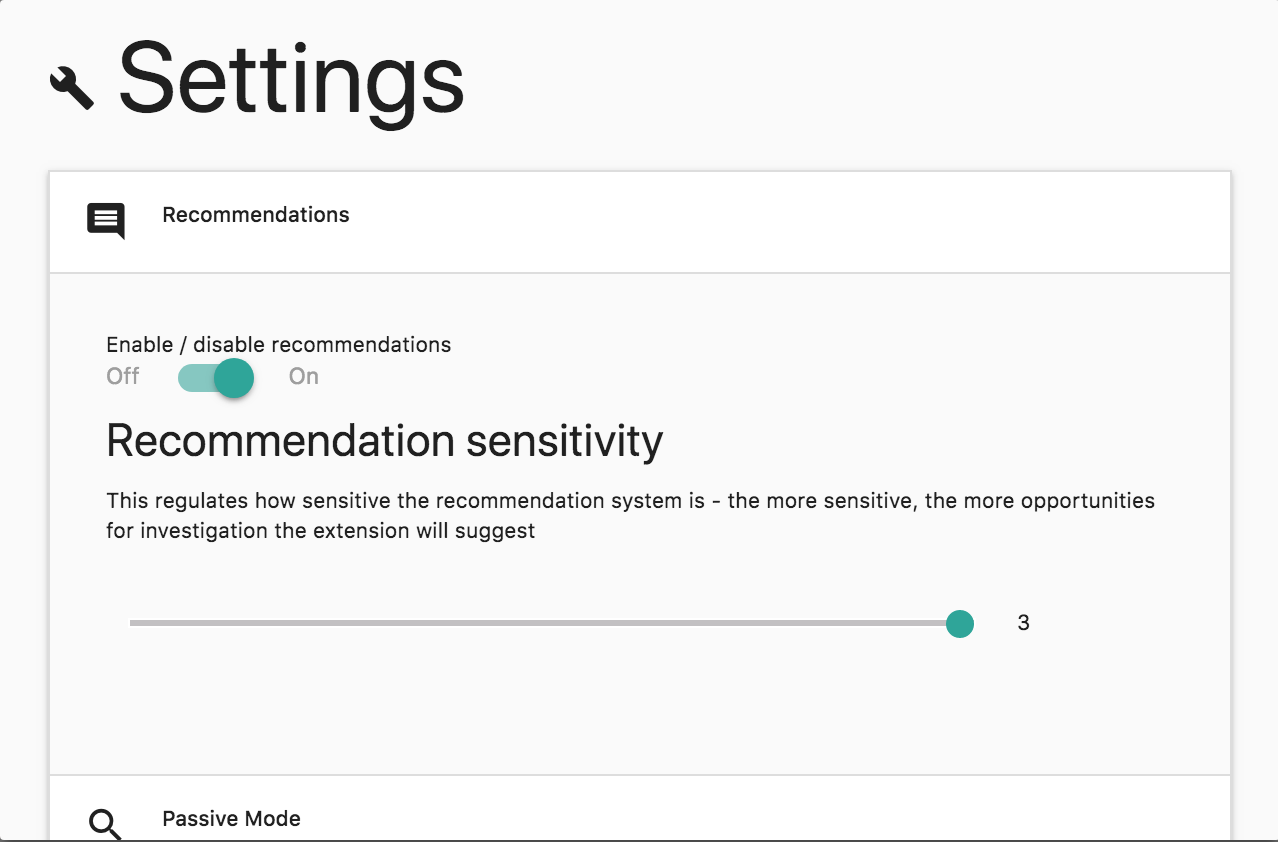
\includegraphics[width=0.7\textwidth]{images/tweaking_recommender_sensitivity.png}
	\caption{Changing the recommendation sensitivity within the settings tab}
	\label{fig:test}
\end{figure}

This adds a bit more complexity to the method in question - the conventional Javascript and JQuery \texttt{submit()} methods work on form elements only. In order to submit the attack attempt for this sensitivity, I manually submit a request to the base URL of the current window, setting the query parameter with the name corresponding to the name of the input being selected. The value for this query parameter is the attack string with some modifications for correct URL encoding. These are:

\begin{enumerate}
	\item Replace the escaped character \texttt{\%20} with \texttt{+}. URL encoding rules state that for query parameters, a whitespace should be set to the \texttt{+} symbol instead
	
	\item Replace instances of the character \texttt{\&} with its URL encoded equivalent \texttt{\%26} - We are now within the specific value of the query parameter, so the \texttt{\&} character must be encoded, otherwise it would be mistaken for the start of another query parameter value within the overall URL, which breaks the attack.
\end{enumerate} 

\section{Action Replay} \label{actionReplay}

Action Replay is a another attack algorithm that works in a slightly different way. This mode allows a user to use the application as normal, with the expectation that the user narrows down the attack surface to a specific set (or sequence) of inputs. \\

Once the Action Replay mode is enabled, the extension adds a small input button to each page's body to allow the user to begin or terminate a session. A session is split into 2 parts - the recording phase and the replay phase. Once a session begins, it must firstly record the requests and inputs being made by the user. The extension does so by storing requests at the aforementioned array \texttt{ARrequests}. Once the user is happy that they have captured enough of the minimum behaviour required to potentially trigger a vulnerability, they can click the button once again to stop recording the session, thus starting the analysis and replay phase of the algorithm. At this stage the algorithm iterates through each of the requests stored in the \texttt{ARrequests} array and appends all of the captured user-controlled inputs to a list of custom \texttt{userInput}s to analyse. A meaningful user-controlled input in this case is either a \textbf{cookie}, a query \textbf{param}eter or a \textbf{header}. The \texttt{userInput} type has the parameters as defined for the data structure \texttt{potentialXSS} (see \ref{storageSpecs}). \\

\begin{figure}[h]
	\centering
	\begin{subfigure}{.5\textwidth}
		\centering
		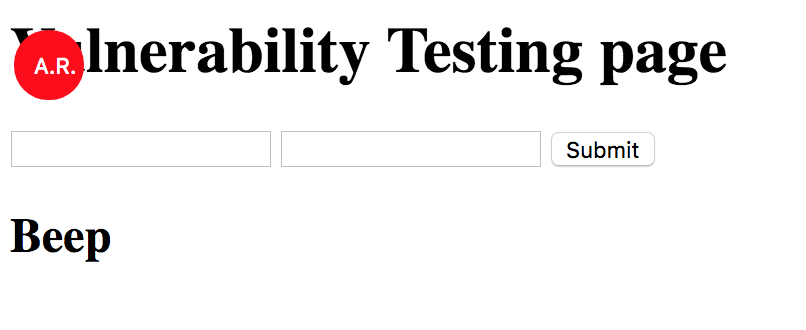
\includegraphics[width=.8\linewidth]{images/ar_initial.png}
		\label{fig:test_page_investigate_form}
	\end{subfigure}%
	\begin{subfigure}{.5\textwidth}
		\centering
		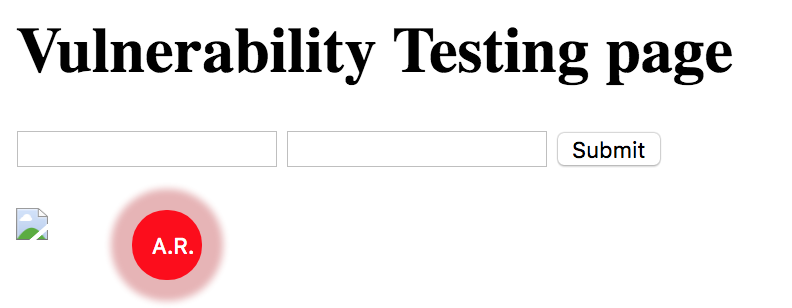
\includegraphics[width=.8\linewidth]{images/ar_recording.png}
		\label{fig:whiteBox}
	\end{subfigure}
	\caption{The Action Replay button before and during a session recording. A recording session starts and stops at the click of this button. In the interest of usability, the button can be moved by the user anywhere on the page so as to not obstruct other content indefinitely.}
	\label{fig:test}
\end{figure} 

In the interest of demonstrating a minimum behaviour within the time frame of the project, I analyse only the responses with the \texttt{Content-type} header set to \texttt{text/html}. This is because vulnerabilities in HTML responses are more readily detectable and easier to analyse than others (e.g. those in CSS files). \\

Once the algorithm has gathered this information, it filters out a series of user inputs it does not deem to be harmful through some heuristics. I focussed on detecting Cross Site Scripting (XSS) vulnerabilities, so the heuristics aim to detect any use of angled brackets (URL encoded or not) alongside potentially executable HTML tag names (such as \texttt{iframe}s, \texttt{img} tags or \texttt{script}). If a \texttt{userInput} is deemed to be potentially dangerous, I store these in the \texttt{potentialXSS} array and send a message to the extension warning of a detected reflection in the outputs. \\

After this intermediary warning, assuming some potentially dangerous user-controlled inputs were found, the algorithm begins to replay the requests, attempting different attacks from a stored suite. For each of the potentially dangerous inputs found earlier, it will apply each of the attacks. To do this, similarly to the process described at \ref{recommendations}, a new window is open, setting the user input to the specific attack value to test whether the attack worked on not. Accordingly, each attack is self-contained, so if it triggers a vulnerability (and Javascript was executed for example), it will (by design) refer itself to the \texttt{request\_logger}, which logs the vulnerability as described before.


\section{Passive Mode}

Passive Mode is designed to run in the background while browsing, gathering data about websites being visited and analysing requests to highlight warning signs of different vulnerabilities. It does so without making any requests of its own, meaning any potential misuse of a web application is entirely dependent on how the user navigates and uses it - this mode simply highlights information the user already has open access to. \\

Once this mode is enabled, any eligible web requests are firstly stored in the \texttt{passiveModeRequests} structure in \texttt{chrome.storage.local}. The analysis is then ran separately per request. The scope of the analysis depends on the activated settings; by default each request is checked for weak security header settings and for potentially dangerous user-controlled inputs that are reflected in responses. The user can also activate further basic CSRF and Cookie safety checks, as well as enabling the \textit{cross checks} feature. 

\subsection{Header Analysis}

This performs some basic checks regarding a set of headers whose presence is designed to improve security in a website. These are:

\begin{itemize}
	\item \textbf{Content-Security-Policy} - This header specifies what sources it trusts content from, in a whitelist manner. XSS attacks abuse the trust that is often (unintentionally) conferred to the source of executable content in a page. With the correct settings, the CSP header will only allow scripts from trusted sources to run. At the same time, since you can specify specific sources as trusted, you can enforce that all content is loaded using SSL by specifying a source with a HTTPS scheme.
	
	\item \textbf{Referrer-Policy} - This policy controls what information to send (if any) on the \texttt{Referer} header\footnote{ Typo intended \cite{refererHeader}}. Many websites use the \texttt{Referer} header to analyse where their traffic comes from, and some even use this to validate permissions to access secure content. However, this may leak sensitive information - this header will usually include the URL of the page which the user was just on. It's often the case that a session ID or other sensitive query parameter is included in the URL, and leaking this information to another website indiscriminately could pose a security risk. The most strict of potential policies here is the \texttt{no-referrer}, which passes forward a blank \texttt{Referer} header. Other, more relaxed alternatives to this policy also exist \cite{referrerPolicy}.
	
	\item \textbf{Strict-Transport-Security} - 	This header (abbreviated to \texttt{HSTS}) allows browsers to determine whether a website should be only accessed using HTTPS or not. There is a small window for a man-in-the-middle attack when using this - if it is the user's first time accessing the website and they access the HTTP version, it is possible for an attacker to hijack their connection and instead connect them to a duplicated site, which allows their credentials to be stolen. Otherwise, as long as the user has visited the safe HTTPS version of the website in question at least once, the \texttt{HSTS} header will have let the browser remember that this website wishes its users to connect to it only through HTTPS, enforcing this for as long as the \texttt{max-age} directive within the header value allows. Additionally, it is recommended that a website also includes the \texttt{includeSubDomains} directive so that any subdomains belonging to this website also enforce a similar policy.
	
	\item \textbf{X-Content-Type-Options} - This header is set to ensure that a defined \texttt{MIME-type} is followed and not changed by a browser. In some cases where the browser is not certain about what content it has just received, it may try to guess this type, which can result in the execution of some (potentially malicious) content. This is called \textit{MIME-type sniffing}, and setting this header to \texttt{nosniff} prevents the browser from doing so.
	
	\item \textbf{X-Frame-Options} - This header can be set to determine whether a website may be rendered in another origin within a \texttt{<frame>}, \texttt{<iframe>} or \texttt{<object>} tag \cite{xFrameOptions}. Denying this behaviour can prevent clickjacking behaviour, where the content from a legitimate website is rendered on a malicious website to trick users into believing they are using the legitimate site.
	
	\item \textbf{X-XSS-Protection} - This is a slightly older header whose behaviour may be made redundant through appropriate use of the \texttt{Content-Security-Policy} header. Nonetheless, setting this header allows the browser to perform basic checks to prevent against reflected XSS attacks, and, depending on the mode set, will sanitize or block the page from being rendered altogether.
	
\end{itemize}

The analysis of these headers does not require that the "recommended" values of these headers are set - although these are \textit{probably} the desired values to be set by the developers, we cannot be sure it isn't intentional on their part to do so. Instead, the extension warns when these headers have not been set, which is a higher indicator of negligence to their importance than a "weaker" setting. If that is the case, an appropriate warning is added to the request in the \texttt{passiveModeWeakHeaderRequests} structure. The \texttt{popup} page will render all the warnings for a request as appropriate. 

\subsection{Reflected Input Checks}

The process performed here is the same as the analysis part described in the Action Replay section \cite{actionReplay}. A difference between these is that any warnings found in this part will be generated and displayed in the \textit{Passive Analysis} tab in the extension, as opposed to the \textit{XSS} tab.

\subsection{Basic CSRF Checks}




%Mention about 2 different ways of doing it - passive mode with normal cross checks by default - sliding window with eviction of requests.
%Instead I keep window size and cross check only when enabled.


\chapter{Applications}

This section provides practical examples through which this extension shows itself to be useful and relevant in fulfilling its purpose of detecting vulnerabilities in websites. Firstly, we will demonstrate how the \textit{Recommendations} feature can be used as a low effort entry point into analysing websites for potential vulnerabilities. Secondly, we will use our Test Harness to demonstrate the uses of the \textit{Action Replay} feature in tweaking and replaying innocent requests to produce behaviour that exposes vulnerabilities on a website. We then show how the \textit{Passive Mode} behaves by showcasing how it performs against the intentionally vulnerable test page. Each of these sections will begin with a preamble covering how the example we will go through is vulnerable to establish a better understanding on how the extension exposes said vulnerability. Finally, we run through a case study of a live website vulnerability that we discovered and exploited as a result of using the extension on it.

\section{Recommendations} \label{applications_recommendations}

In order to set up the example to demonstrate a use case of the \textit{Recommendations}, we set up the Test Harness with 2 intentional XSS Vulnerabilities that work in the same way - any input that is submitted in either the \texttt{injection} or \texttt{injection2} input fields is reflected on the page below its respective input (in the \texttt{output} and \texttt{output2} fields respectively). The source code of the page at this point is shown in Listing \ref{lst:test_harness}, and the resulting rendered page is shown in Figure \ref{fig:test_harness_default}. \\


%\begin{minipage}{\linewidth}
\begin{lstlisting}[label={lst:test_harness}, language={HTML}, caption={The HTML contents of the Test Harness for this example. Two of the inputs in the page are reflected onto the page when they are submitted as query parameters (i.e. seen in the page URL)}]
<script>
	window.onload = function() {
		var url = new URL(window.location.href);
		
		var c = url.searchParams.get("injection");
		if (c) {
			document.getElementById("output").innerHTML = c;
		}
		
		var d = url.searchParams.get("injection2");
		if (d) {
			document.getElementById("output2").innerHTML = d;
		}
	}
</script>

<h1>Vulnerability Testing page</h1>

<form id="boop" action="">
	<input type="text" name="injection" value=""/>
	<input type="text" name="unused" value="">
	<input type="submit">
</form>
<h2 id="output"></h2>

<form id="beep" action="">
	<input type="text" name="unused" value=""/>
	<input type="text" name="injection2" value="">
	<input type="submit">
</form>
<h2 id="output2"></h2>
\end{lstlisting}
%\end{minipage}



\begin{figure}[h]
	\centering
	\begin{subfigure}{.45\textwidth}
		\centering
		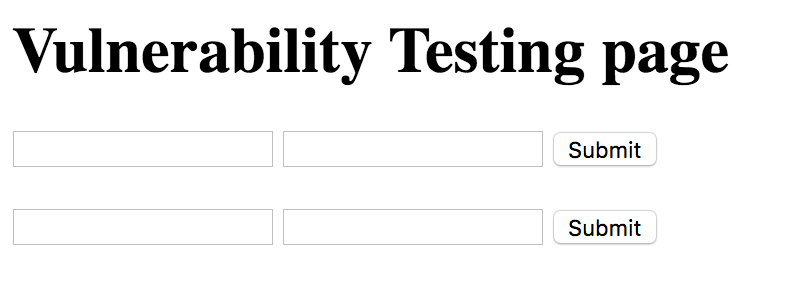
\includegraphics[width=.8\linewidth]{images/test_harness_recommendations.png}
		\label{fig:test_harness_original}
	\end{subfigure}%
	\begin{subfigure}{.6\textwidth}
		\centering
		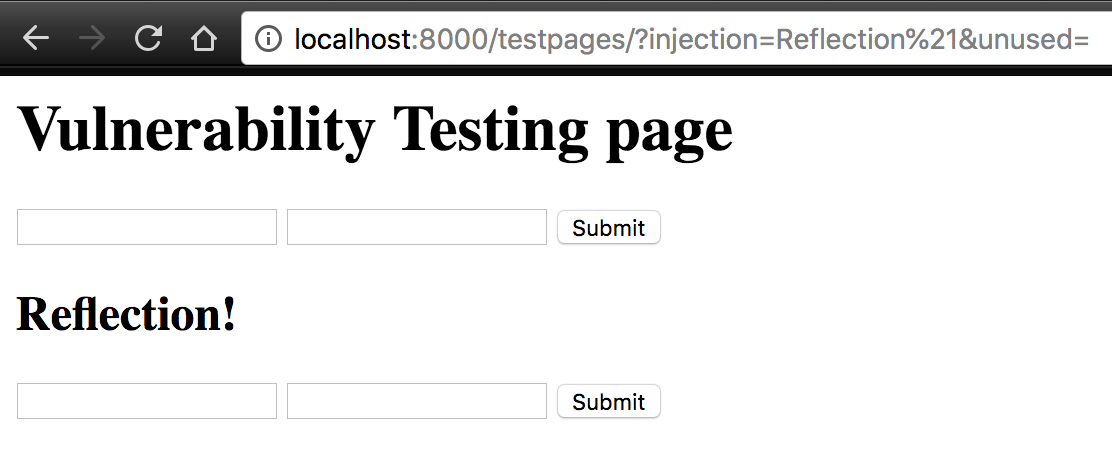
\includegraphics[width=.8\linewidth]{images/test_harness_reflection_1.png}
		\label{fig:test_harness_reflection_1}
	\end{subfigure}
	\caption{The default Test harness page to demonstrate XSS vulnerabilities. Submitting the first input causes the reflection in the second image.}
	\label{fig:test_harness_default}
\end{figure} 

Now we enable the recommendations in this page - setting the sensitivity parameter to \textbf{1}. At this stage, one input is added per form on the page, encouraging the user to "investigate" the first input on each of the forms, seen in Figure \ref{fig:test_harness_recommendations_2}. 

\begin{figure}[h]
	\centering
	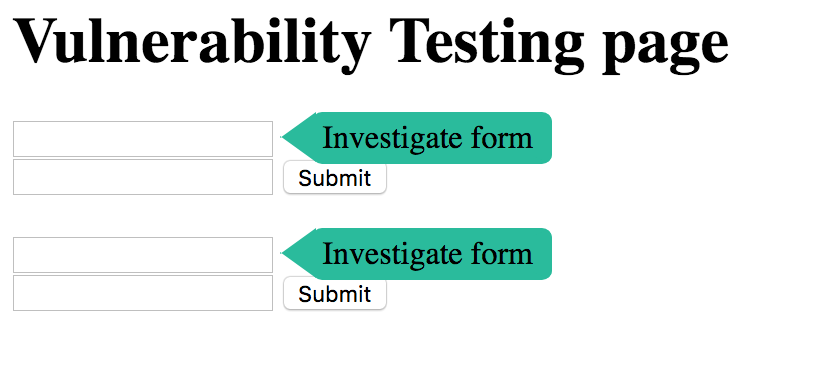
\includegraphics[width=0.7\textwidth]{images/test_harness_recommendations_2.png}
	\caption{Enabling the recommendations on the Test Harness}
	\label{fig:test_harness_recommendations_2}
\end{figure}

If the user decides to test the first input on the page, one of the attempted attacks will inject the following into the input:

\begin{center}
	\texttt{<img src=a onerror="window.location.replace( 'chrome-extension://ID/request\_logger.html?ref=CURRENT\_URL')">}
\end{center}

where the \texttt{ID} parameter is replaced by the ID given by Chrome to the extension, and the \texttt{CURRENT\_URL} is the current web address before the form was submitted. This is an example of an XSS attack which surreptitiously executes Javascript on a page by injecting an \texttt{<img>} tag with an invalid source location. This triggers an error when the image is later loaded on that page (since we have established that this input is reflected back onto the page). At this point, the \texttt{onerror} callback given to the input is executed, and in our case, will change the location of the current page to our previously mentioned \texttt{request\_logger} page, passing the current URL as a query parameter in this referral. \\


The \texttt{request\_logger} page is equipped to deal with this specific type of request, by alerting the user both through the extension and in the page output that an XSS vulnerability has been found, indicating the address of the culprit page. The only (current) means to reach this page in the extension is through the payloads prepared in the attacks, meaning that Javascript had to have been executed by one of these, thus indicating an XSS vulnerability. Upon opening the extension for further details, the initial Test Harness URL is then listed as a website vulnerable to XSS. \\


\begin{figure}[h]
	\centering
	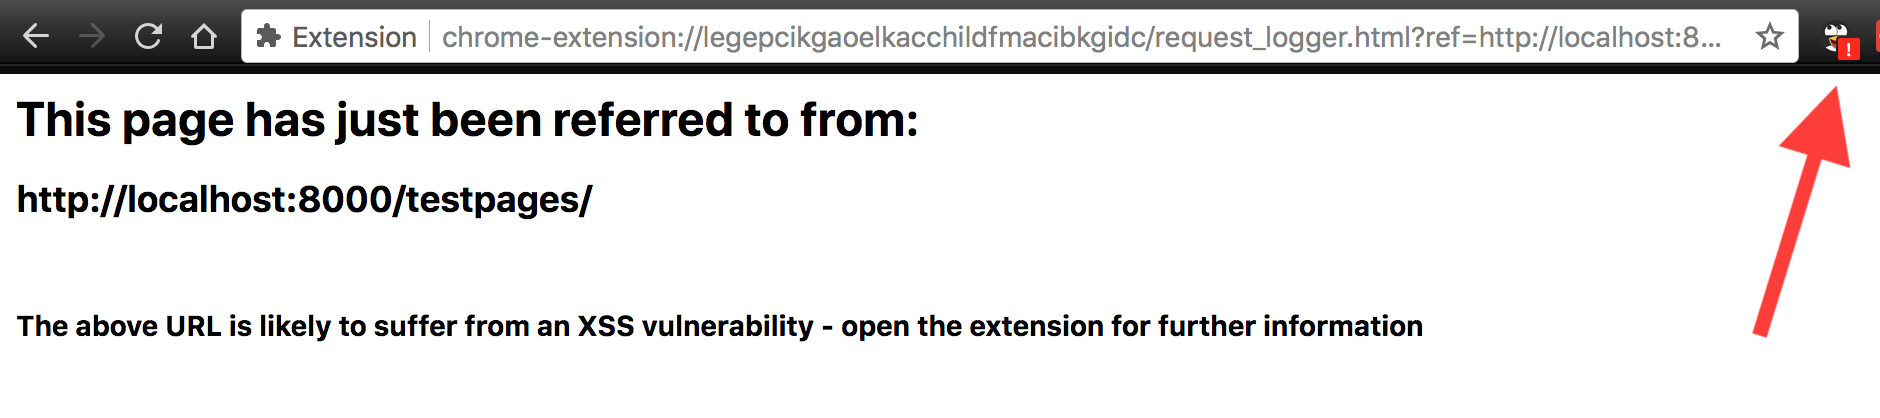
\includegraphics[width=	\textwidth]{images/request_logger_warning.png}
	\caption{The request logger page warns the user that the reason they've reached this page is likely to have been due to an XSS vulnerability. Note that the extension badge is also updated with a warning \textbf{(!)} label to indicate this (arrow added in diagram for emphasis).}
	\label{fig:request_logger_warning}
\end{figure}

\begin{figure}[h]
	\centering
	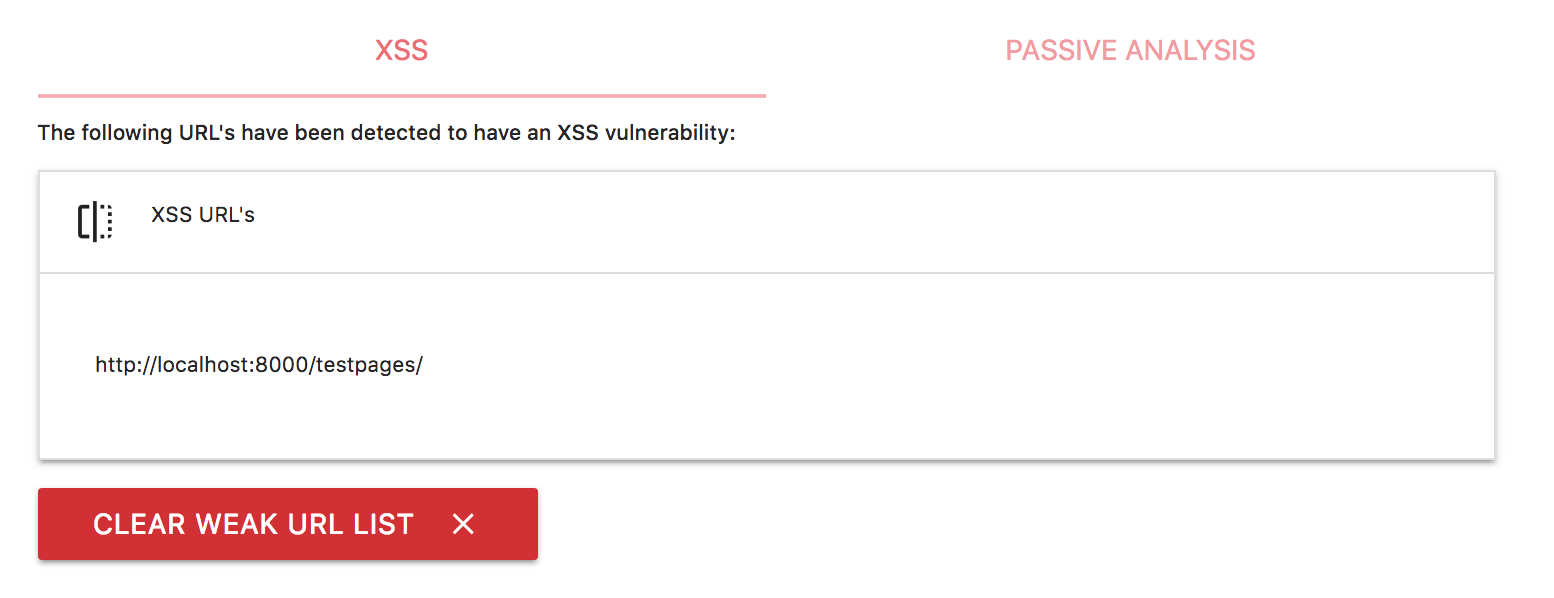
\includegraphics[width=	\textwidth]{images/xss_vulnerable_url.png}
	\caption{Opening the extension confirms that the suspicious URL was indeed vulnerable to XSS.}
	\label{fig:xss_vulnerable_url}
\end{figure}

However, this has only covered one of the vulnerabilities on the page - there is still another vulnerability in the last input on the page, which is reflected in the same way as above. However, clicking the second \textit{Investigate Form} button in this case will not reveal anything about the last vulnerable input - it will only attack the first input in the second form on the page. This attack results in nothing besides the submission of the second form and the reloading of the page. This emphasises the need for a Recommendation Sensitivity setting - if we change it from \textbf{1} to \textbf{2}, more suggestions are added to the page (1 for every \texttt{<input>} tag); we can now attack the last input. This results in a vulnerability detection process very similar to the one described above for the other input.   

\section{Action Replay}

Now we consider how we can use the Action Replay algorithm to automatically replay attacks on focussed inputs and requests. \\

The vulnerability in this example is the same as the one from the \textit{Recommendations} section (\ref{applications_recommendations}) - the website suffers from a reflected XSS vulnerability. Here, we assume that through use of the website, the user has noticed there may be a vulnerability present, and attempts to exploit the website. Perhaps they attempt a similar injection as before to test their hypothesis:

\begin{center}
	\texttt{<img src=a >} 
\end{center}

Upon trying this input, they are confronted with the page shown in Figure \ref{fig:action_replay_initial}. \\

\begin{figure}[h!]
	\centering
	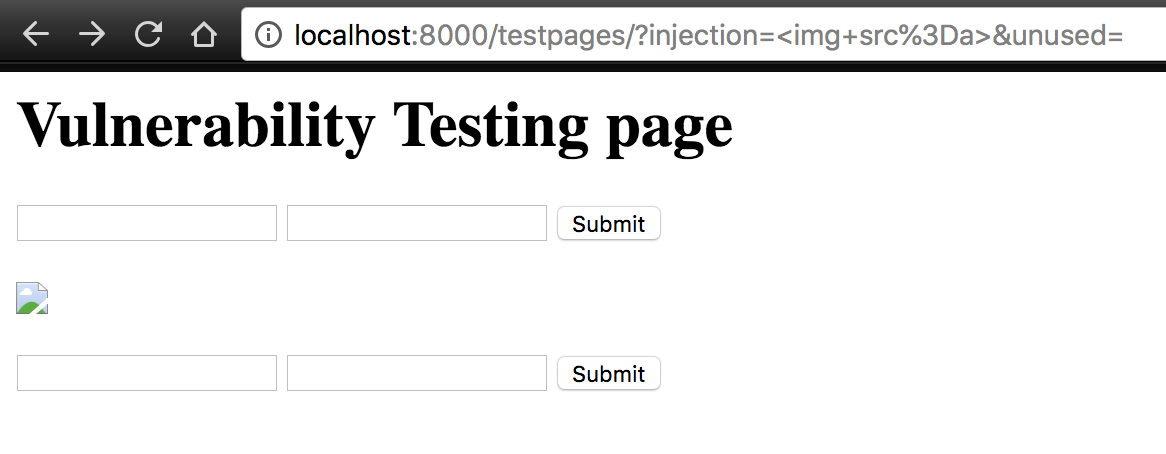
\includegraphics[width=0.7\textwidth]{images/action_replay_initial.png}
	\caption{Injecting \texttt{<img src=a>} into an input results in this page}
	\label{fig:action_replay_initial}
\end{figure}

To a web security analyst with a more trained eye, this may present a security risk, as they were freely able to inject a HTML tag into the page of their choosing. It is at this point where they decide to focus on this particular input and activate the Action Replay. After enabling and starting a recording, they reattempt the earlier injection (Figure \ref{fig:action_replay_attack}). \\

\begin{figure}[h!]
	\centering
	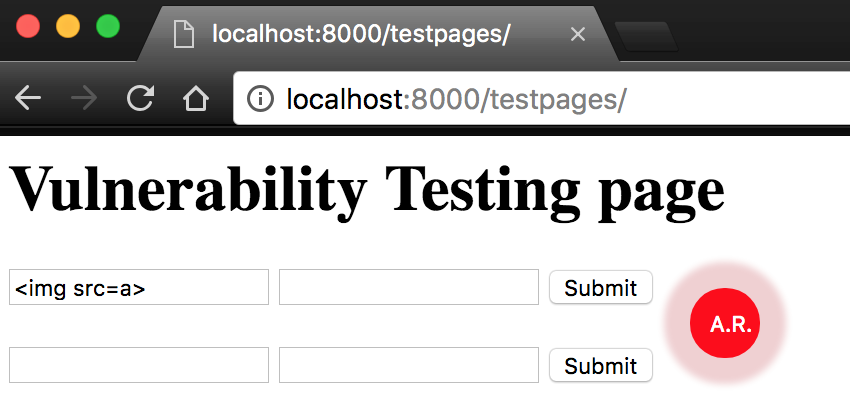
\includegraphics[width=0.7\textwidth]{images/action_replay_attack.png}
	\caption{Retrying the attack while recording using Action Replay}
	\label{fig:action_replay_attack}
\end{figure}

Once the new page loads, the user can then stop the recording by clicking the \textit{AR} button once again. At this point, the analysis and automated replay begins. If the algorithm has appropriately detected a set of potentially dangerous inputs it can override to begin an attack, then almost immediately after finishing the recording, Chrome will open several new windows, each of which attempts an attack. Not all of these are expected to yield successful vulnerability identifications, but, for this example, we see that one of the resultant tabs has ended up in the \textit{Request Logger} page. This can only indicate that the payload of one of the attacks was successful (Figure \ref{fig:successful_replay}). \\ 


\begin{figure}[h!]
	\centering
	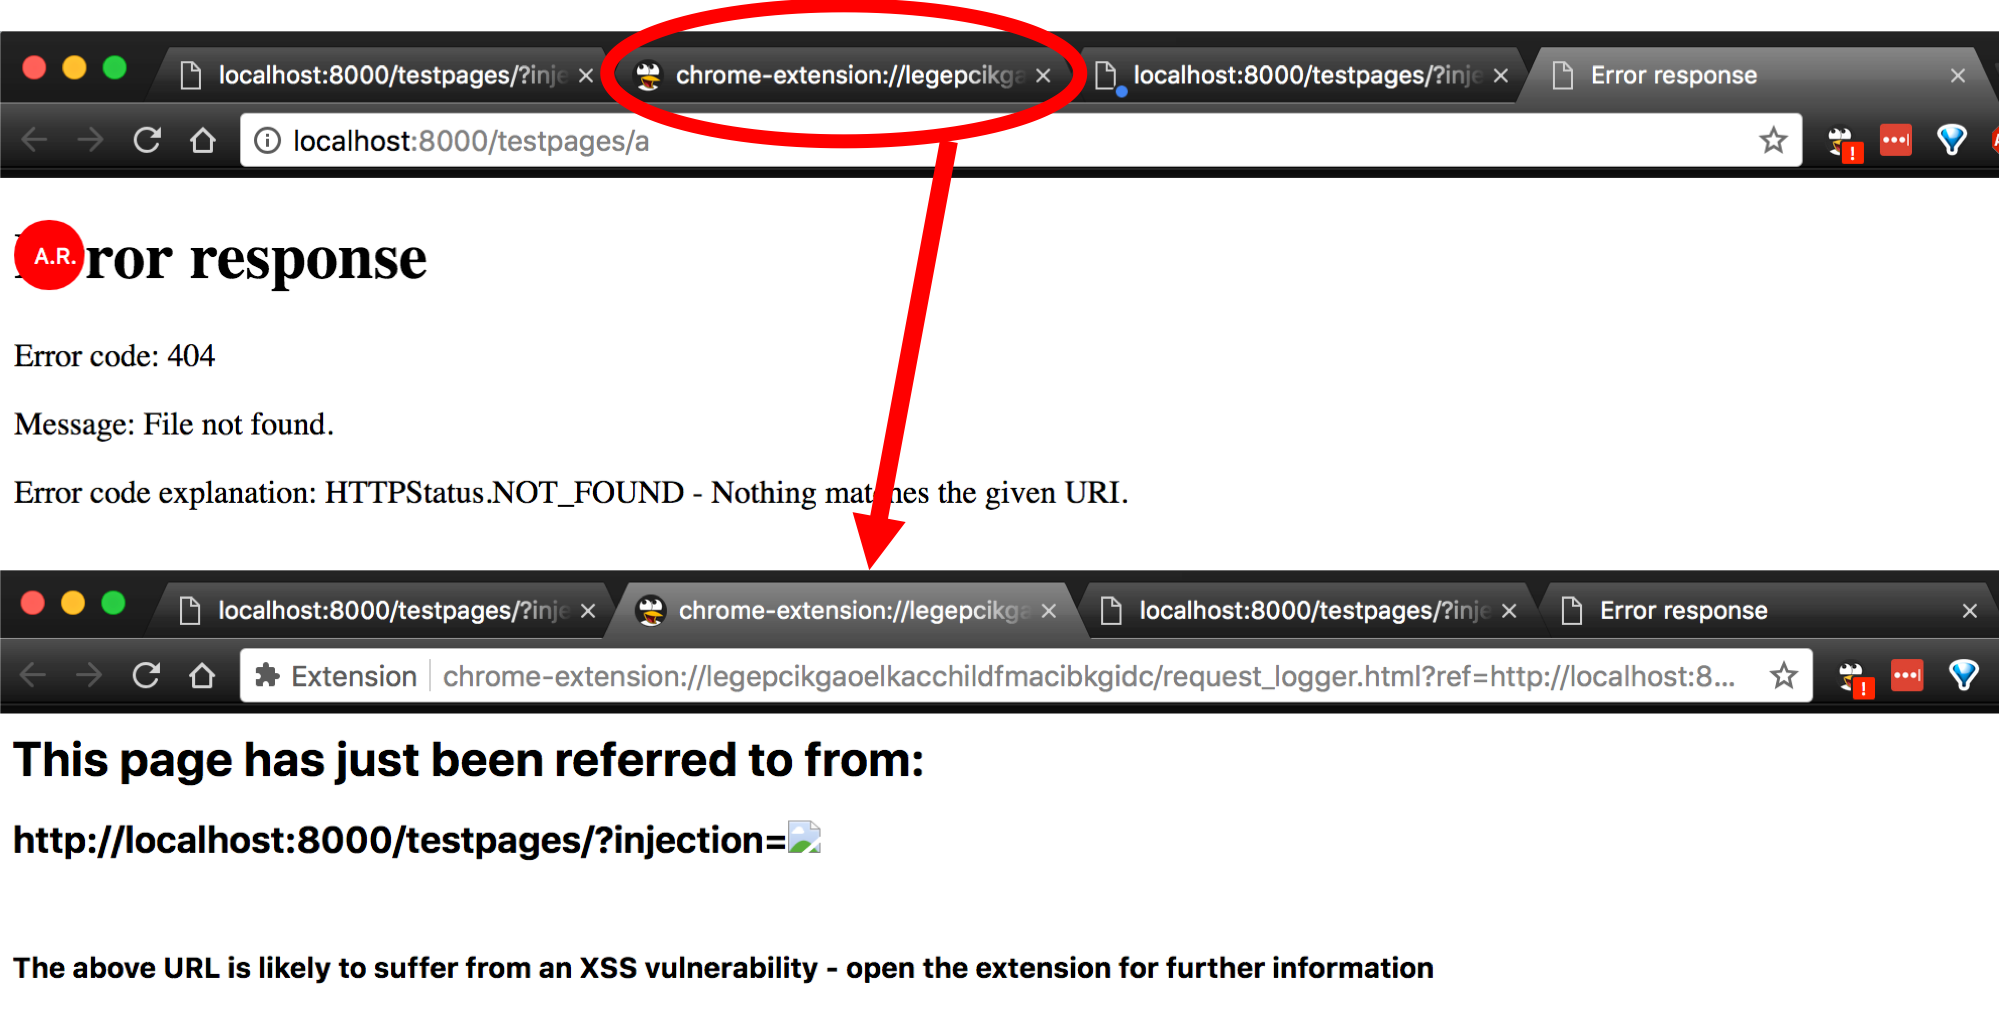
\includegraphics[width=\textwidth]{images/successful_replay.png}
	\caption{The Action Replay generates the outputs of several attacks in new windows. The 2nd of the inspected windows showcases a successfully detected vulnerability that executed a Javascript payload.}
	\label{fig:successful_replay}
\end{figure}

As before, once this stage is reached, we have the appropriately reported information in the extension. The list of URLs that suffer from XSS vulnerabities is updated, containing the latest victim. Additionally, Action Replay publishes a list of inputs it considered to be dangerous, showing the user which inputs were targeted by the automated attacks (Figure \ref{fig:dangerous_inputs}).  \\

\begin{figure}[h!]
	\centering
	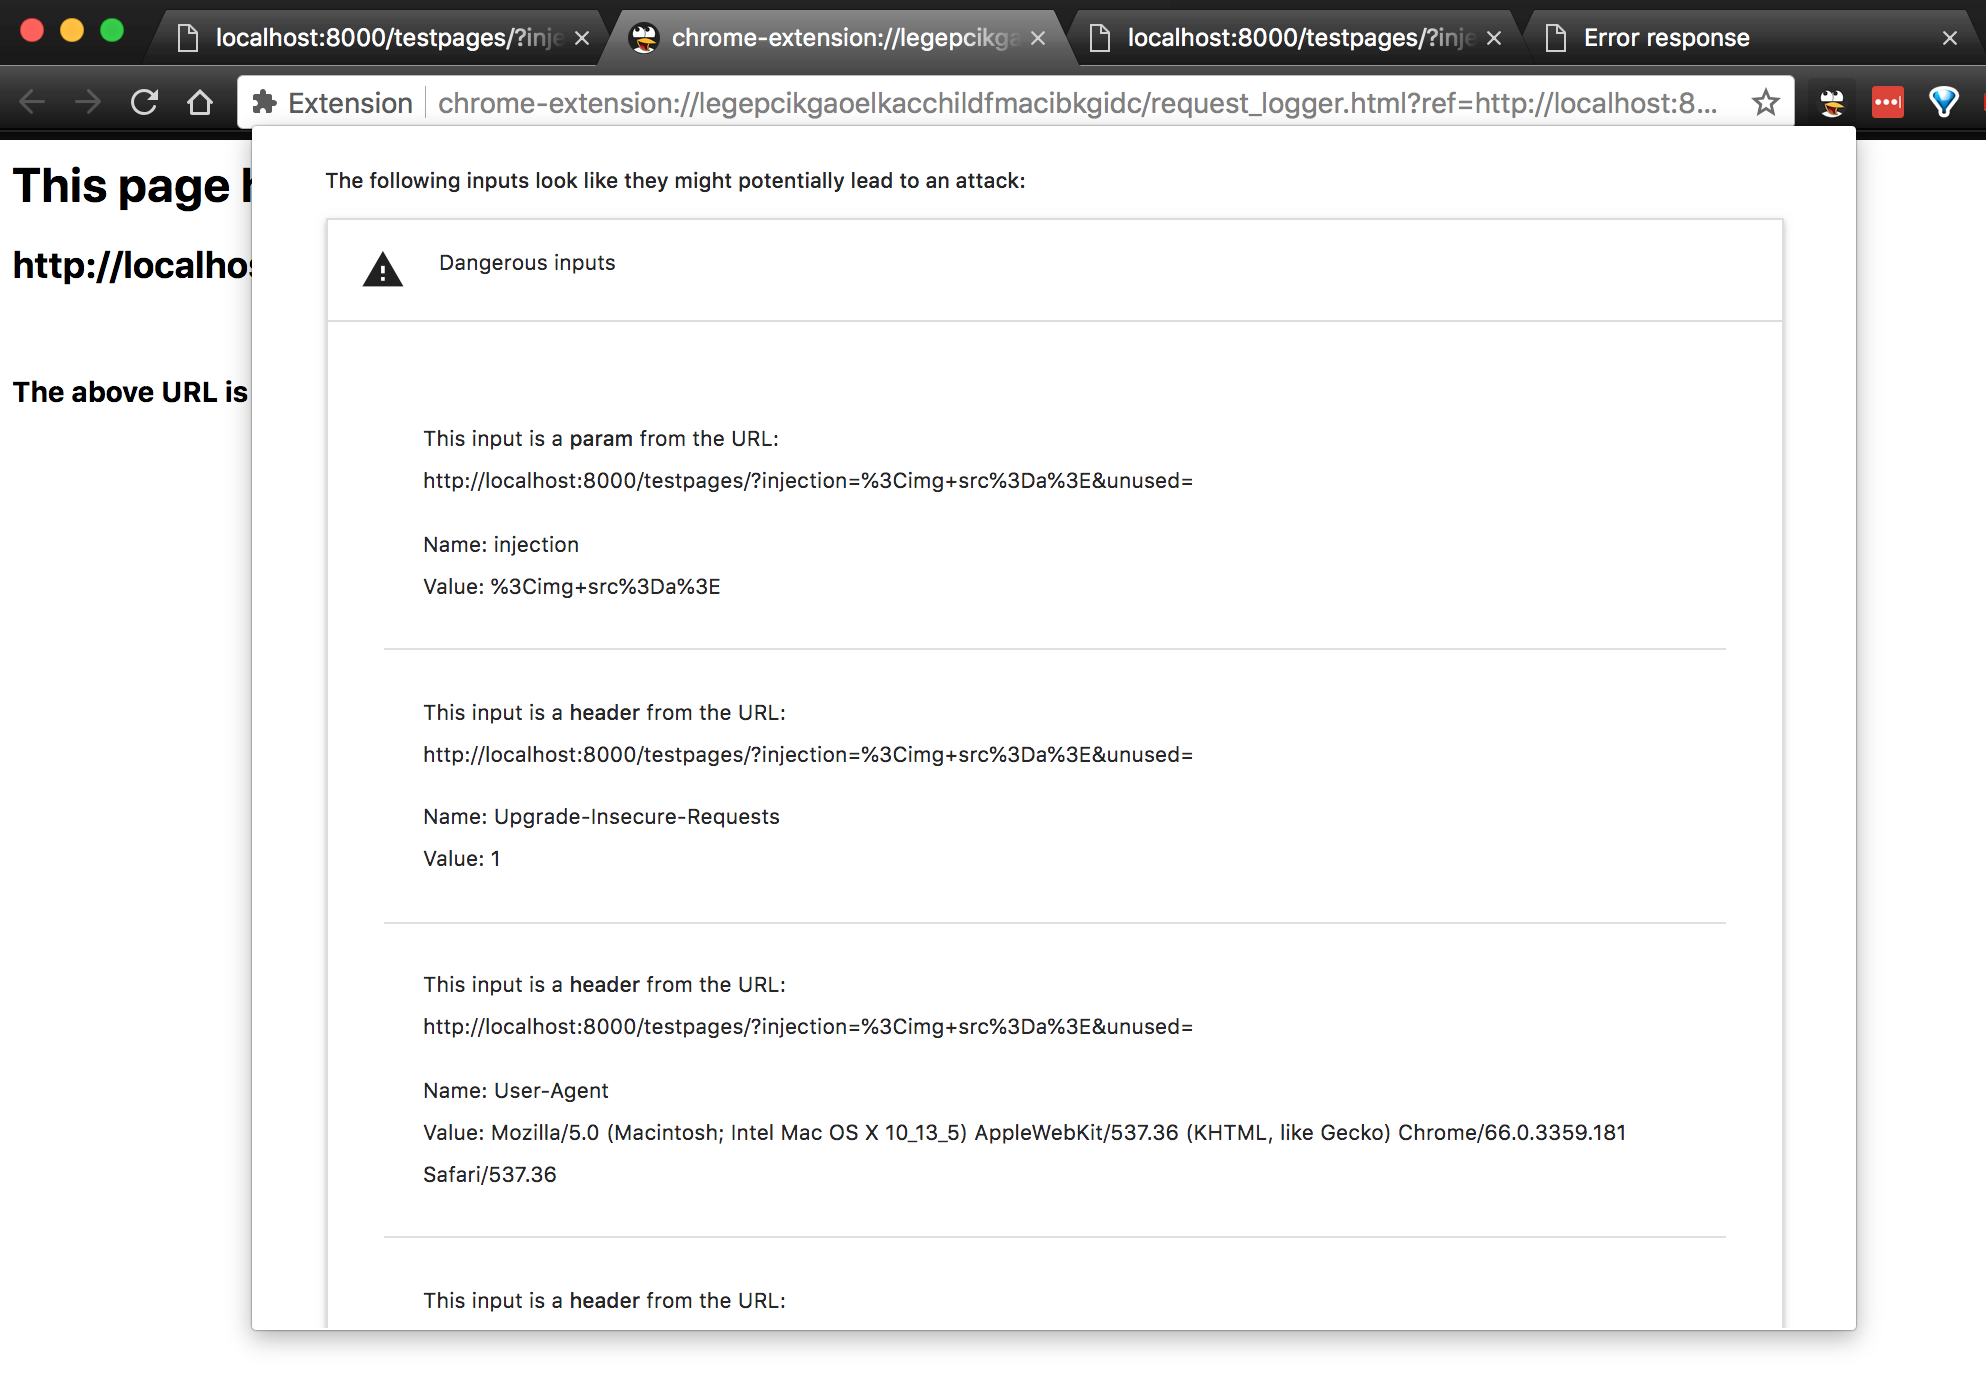
\includegraphics[width=\textwidth]{images/dangerous_inputs.png}
	\caption{The Action Replay outputs a list of inputs it has considered to be dangerous. In this screenshot, we see the \textbf{param} with the name \textbf{injection} is one of the potentially dangerous inputs. }
	\label{fig:dangerous_inputs}
\end{figure}

\section{Passive Mode}

We now review the Passive Mode and highlight what useful information it can produce to a user while they use the website in a normal fashion. By default, this mode will check that a set of headers are being sent with each request and response. To demonstrate a worst case scenario of an insecure site, we make no intentional changes to the Test Harness page. As expected, this raises warnings for all of the headers enumerated in section \ref{header_analysis}. The outputs of this scan are shown in Figure \ref{fig:passive_weak_headers_1}. \\

\begin{figure}[h!]
	\centering
	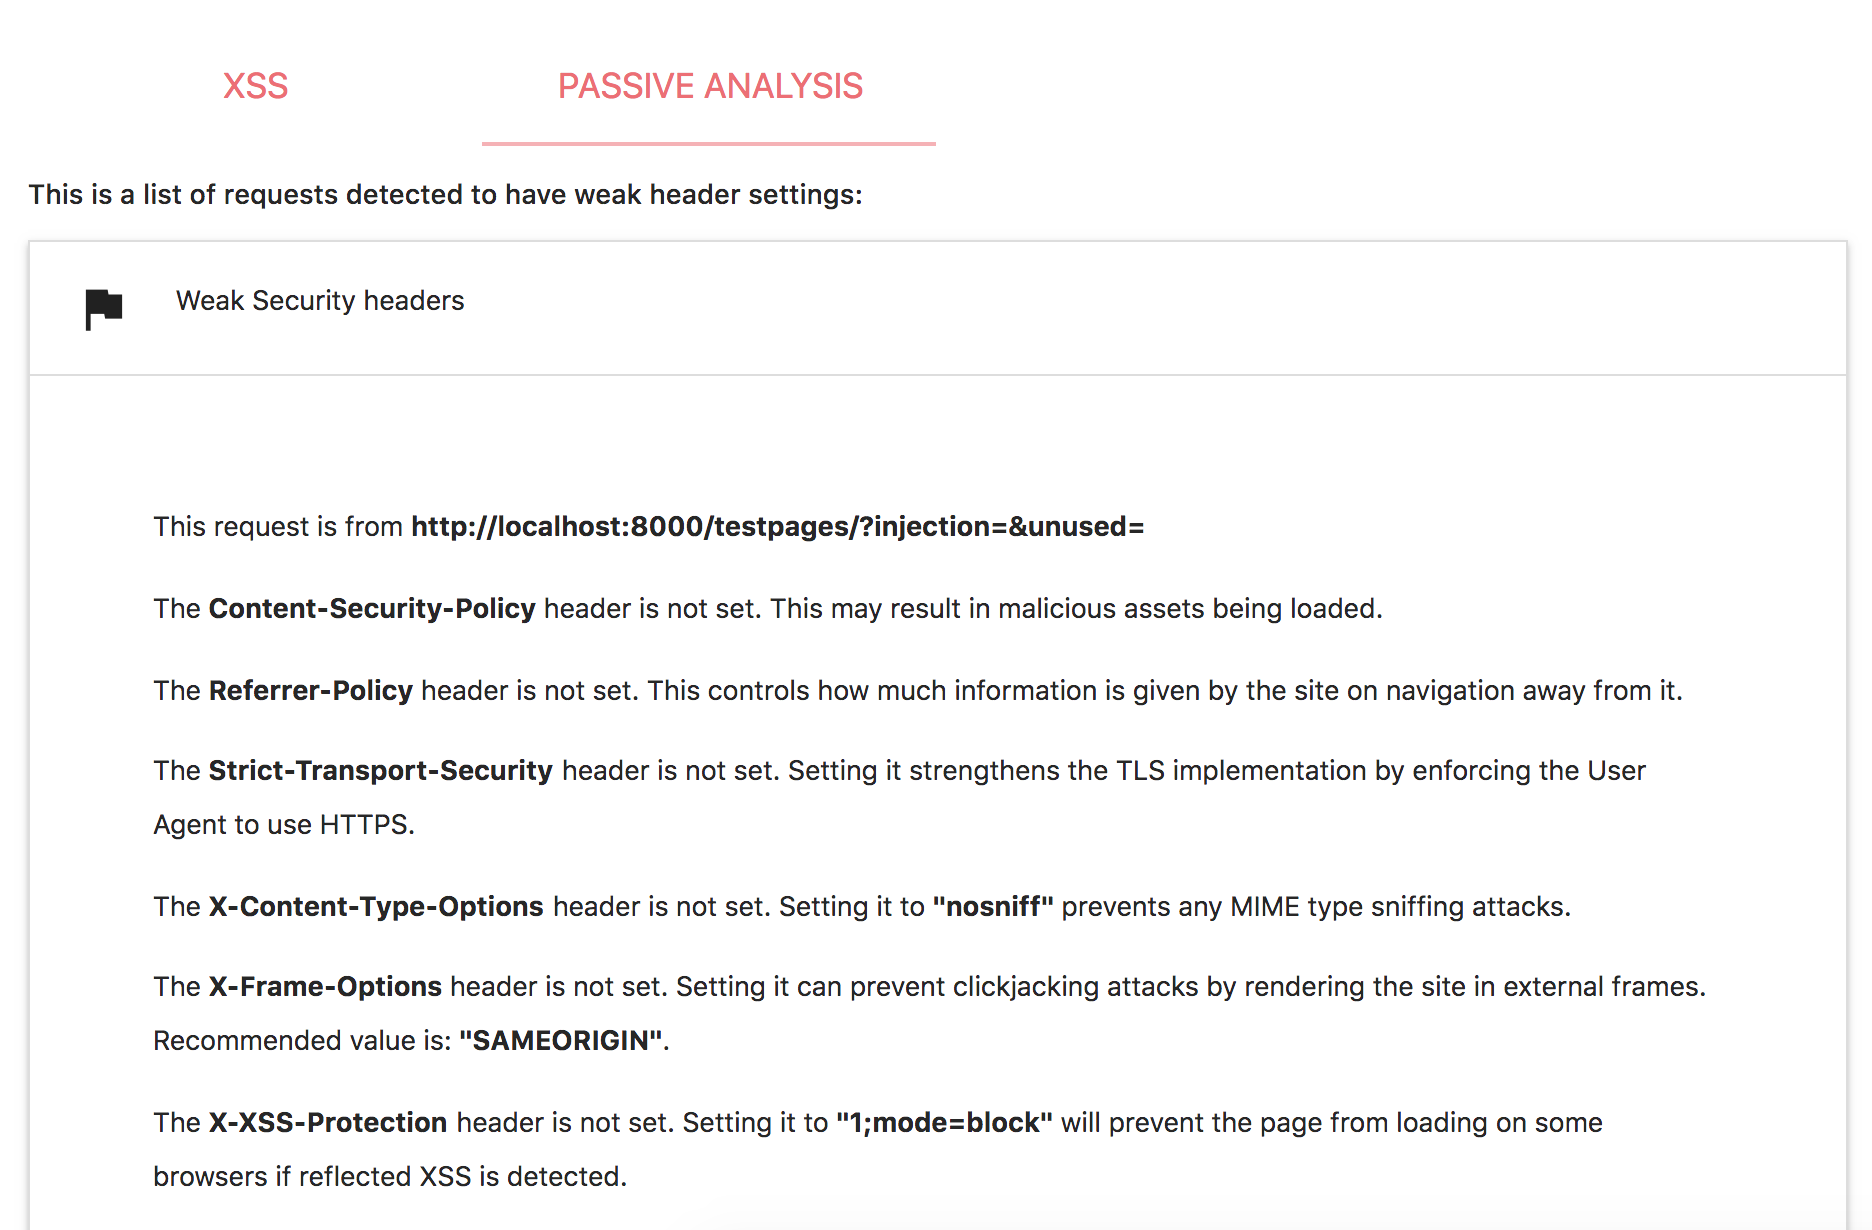
\includegraphics[width=\textwidth]{images/passive_weak_headers_1.png}
	\caption{A webpage which makes no effort to set secure headers (as the Test Harness does here) will raise up warnings by the passive mode in this regard.}
	\label{fig:passive_weak_headers_1}
\end{figure}

If we scan another website however, we are more likely to find a bit more attention to detail in terms of setting secure headers. We scanned \url{http://google.com} and came up with better results than the Test Harness - at least half of these headers had been set to their recommended settings as shown in Figures \ref{fig:google_headers} and \ref{fig:google_headers_2}. \\

\begin{figure}[h!]
	\centering
	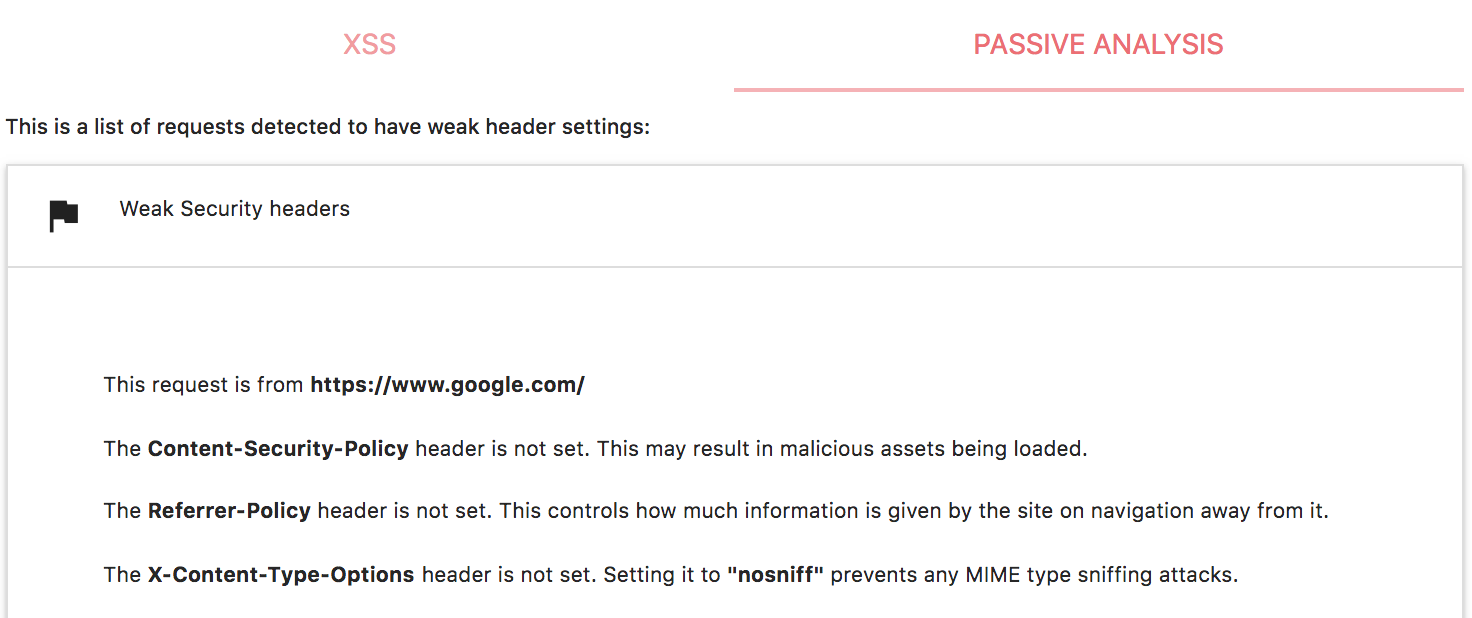
\includegraphics[width=\textwidth]{images/google_headers.png}
	\caption{The header analysis from scanning \texttt{http://google.com} shows that some of the security headers have been set, but others are still unset.}
	\label{fig:google_headers}
\end{figure}

\begin{figure}[h!]
	\centering
	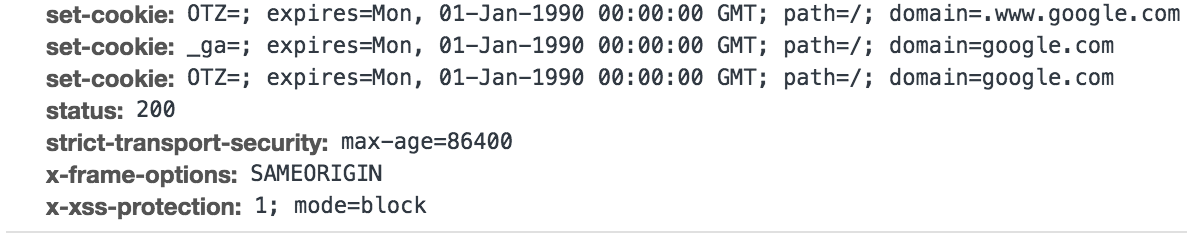
\includegraphics[width=\textwidth]{images/google_headers_2.png}
	\caption{Looking at the request details in the Developer Tools in Chrome reveals that the headers that were not reported by the extension had been set by Google.}
	\label{fig:google_headers_2}
\end{figure}

Besides headers, this mode also checks for potentially reflected user-controlled inputs (much like the Action Replay algorithm). Here we reuse the vulnerabilities from the Test Harness page as a means to test the outputs of this algorithm. As before, we submit the first input, which we know to be reflected on submission. This appends a warning to the log produced for this request, as shown in Figure \ref{fig:passive_reflection}.

\begin{figure}[h!]
	\centering
	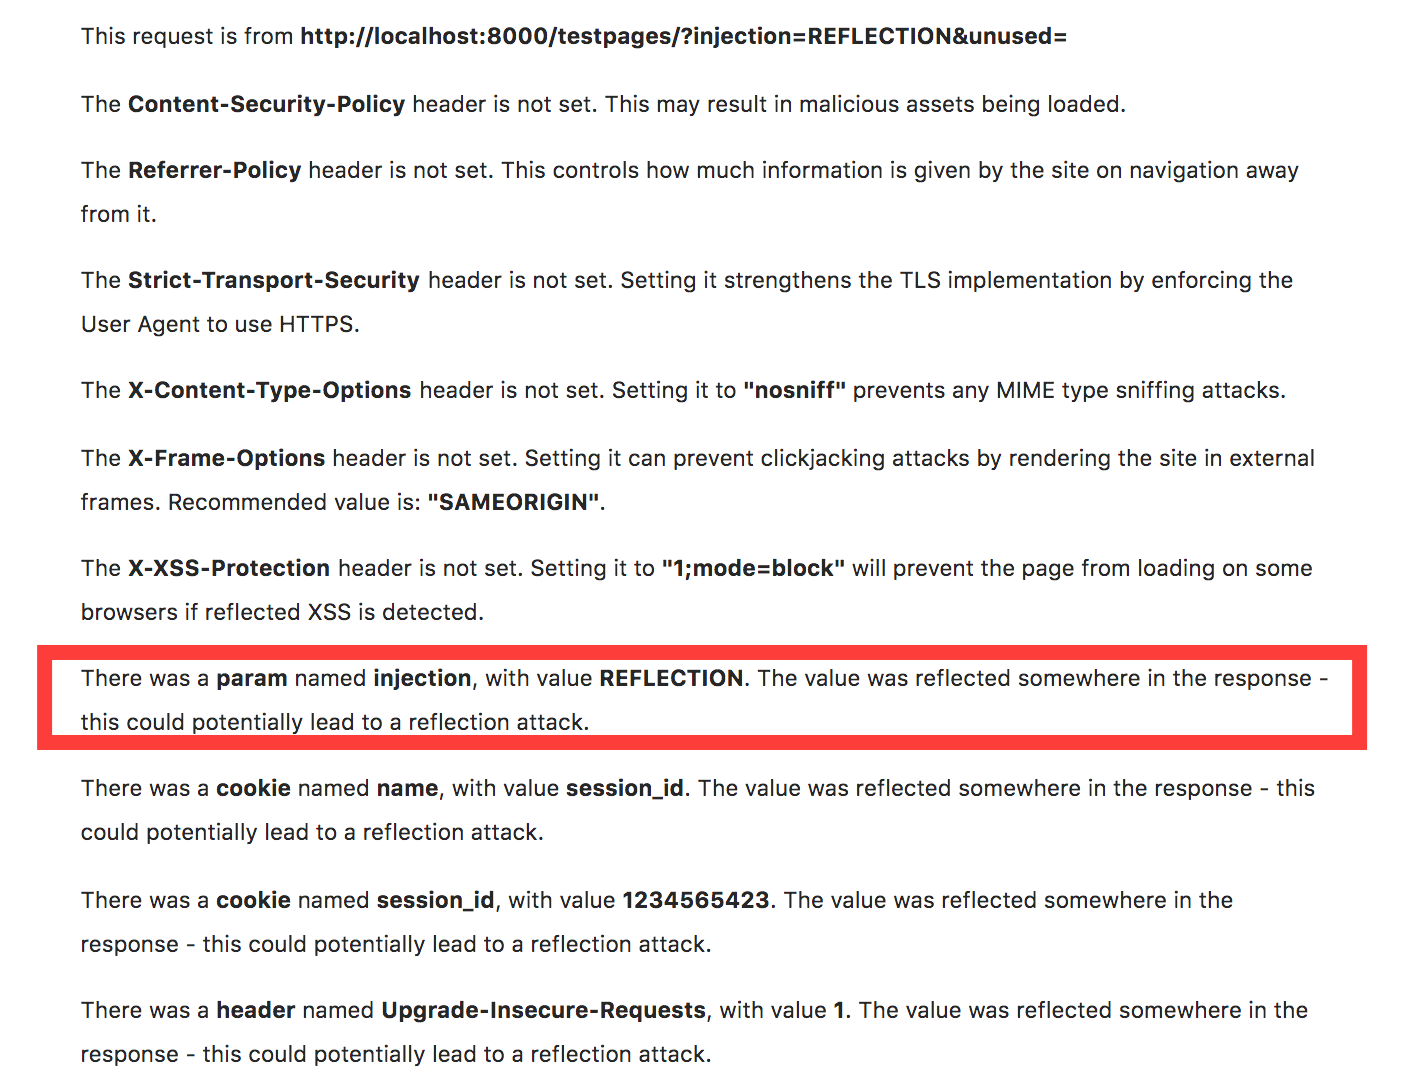
\includegraphics[width=\textwidth]{images/passive_reflection.png}
	\caption{Although this mode is liberal in highlighting potential vulnerabilities, amidst the warnings we see that it has detected the reflected input caused by the query parameter.}
	\label{fig:passive_reflection}
\end{figure}


\subsection{CSRF alerts} \label{applications_CSRF_alerts}

As explained in Section \ref{csrfChecks}, this mode is also equipped to perform some basic checks to alert the user to factors which may facilitate the crafting of CSRF attacks, as long as the correct setting is enabled. To emulate this situation, we add some cookies to the Test Harness using Javascript. One of these is purposefully named with keywords that will trigger our filter that looks for cookies that store session IDs. We add the code in Listing \ref{lst:csrf_cookies} to the Javascript portion of our page.

\begin{lstlisting}[label={lst:csrf_cookies}, language={HTML}, caption={We add some cookies to the page - one of these is designed to trigger our filter to find Session ID related cookies}]
...
<script>
	window.onload = function() {
		...
		document.cookie = "fake_cookie_1=BOOP;"
		document.cookie = "session_id=1234565423";
		document.cookie = "analytics_cookie=BEEP";
	}
<script>
...
\end{lstlisting}

The rest of our Test Harness page already fulfills the minimum requirements for the CSRF alert - it contains forms but none of these are equipped with a hidden \texttt{<input>} tag (which would be expected to be used as an Anti-CSRF token, given that it has a session cookie). This results in the CSRF alert being produced for this page as shown in Figure \ref{fig:csrf_warning}.

\begin{figure}[h!]
	\centering
	
\includegraphics[width=\textwidth]{images/csrf_warning.png}
	\caption{When the website conforms to the minimum requirements previously explained, the passive analysis produces this CSRF warning.}
	\label{fig:csrf_warning}
\end{figure}

\subsection{Insecure Cookie Alerts}

Passive mode can also check whether any potentially important or valuable cookies are being set with the appropriate security settings. Setting up an example to demonstrate this is the same as described in Section \ref{applications_CSRF_alerts} - we will reuse the same 3 cookies for this case. The only seemingly \textit{valuable} cookie in this case is the same, the one that stores the "session\_id" for the user. Only this cookie should raise any alerts about not being set securely. This is what we see shown in Figure \ref{fig:cookie_warning}. As expected, setting one or both of these flags in the cookie will change or delete the warning altogether.  \\

\begin{figure}[h!]
	\centering
	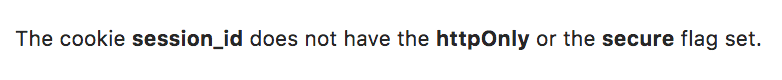
\includegraphics[width=0.85\textwidth]{images/cookie_warning.png}
	\caption{The extension warns of any cookies that may be of particular value to the user experience (such as the session ID) and have not been set with the appropriate security flags.}
	\label{fig:cookie_warning}
\end{figure}



\subsection{Request Cross Checks}

Now we showcase the cross check feature at work. This component has the ability to detect patterns that manifest themselves an arbitrary amount of requests apart. It is designed to find second-order attacks, but we will simulate this in a simpler way - we take advantage of the reflection vulnerability in our test harness to analyse outputs across different requests. In order to demonstrate a convincing enough example of the algorithm at work, we adopt the following strategy:

\begin{enumerate}
	\item After setting up the extension to analyse cross requests, we set the window size to a value of 3. This gives us enough separation to analyse outputs with at least one "uncorrelated" request inbetween.
	
	\item We submit the first form of the Test Harness using both inputs - we use the reflected input as the ongoing vulnerability, and we use the previously \texttt{unused} input in the form to keep track of what request we are on. For the purpose of this example, we submit the \texttt{injection} parameter with the value \texttt{BLUE} and the \texttt{unused} parameter with the value \texttt{Number 1} (as it is our first request).
	
	\item On the resulting page, we now submit the same form using different values for the same inputs - the \texttt{injection} parameter will be \texttt{RED} and the \texttt{unused} parameter will be \texttt{Number 2}.
	
	\item The algorithm generates several pages as a result of comparisons (this is necessary to obtain the resulting output of running the Javascript code that causes the reflections). We select one of these pages and now submit the form with \texttt{injection} to be \texttt{BLUE} again (hence replicating the behaviour of being our "second-order vulnerability") and the \texttt{unused} input as \texttt{Number 3} (as it is our final request).
\end{enumerate}

This strategy should be sufficient to demonstrate an example that showcases the cross request comparison. After executing this, we find the desired results - amongst several other warnings due to a large number of comparison, the extension points out that the \texttt{BLUE} value as seen in the third request (the one where the \texttt{unused} parameter was \texttt{Number 3}) had been already seen as a parameter value back in the first request. A partial screenshot of the results is shown in Figure \ref{fig:cross_check_warnings}. This demonstrates the capacity of using some directed automated techniques to analyse data which may otherwise seem distant; finding this sort of vulnerability with a much larger request window size would be more 

\begin{figure}[h!]
	\centering
	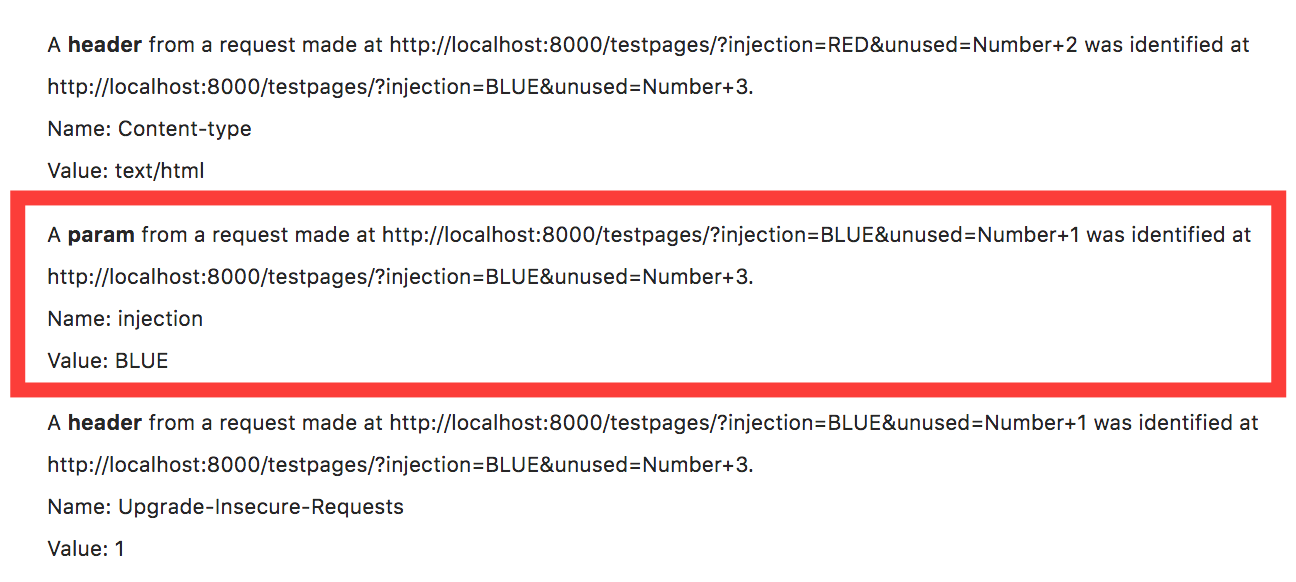
\includegraphics[width=0.85\textwidth]{images/cross_request_warnings.png}
	\caption{The extension finds the reflected exploit across requests with a separating distance of at least 1 other request. The image omits a substantial amount of other warnings.}
	\label{fig:cross_check_warnings}
\end{figure}


\section{Live Vulnerability Test Case}

This section will describe a series of steps taken while using the extension that lead to the discovery of a real vulnerability on a live website. As part of the section we will demonstrate how this vulnerability can further be exploited. The website belongs to a fitness organization based in India; the specific login page we will consider is regularly used by over 1000 gyms / fitness studios. According to \url{alexa.com},\footnote{Not to be confused with Amazon's voice assistant, although both services are owned by Amazon.} this login form accounts for approximately 27\% of the traffic on the main domain. The website is kept anonymous as a courtesy to its rightful owners. \\ 

This particular vulnerability was discovered as a result of using the recommendations feature of the extension. Figure \ref{fig:vuln_page} shows the login form before and after enabling the recommendations in the extension, at a sensitivity of \textbf{2}.

\begin{figure}[h]
	\centering
	\begin{subfigure}{.5\textwidth}
		\centering
		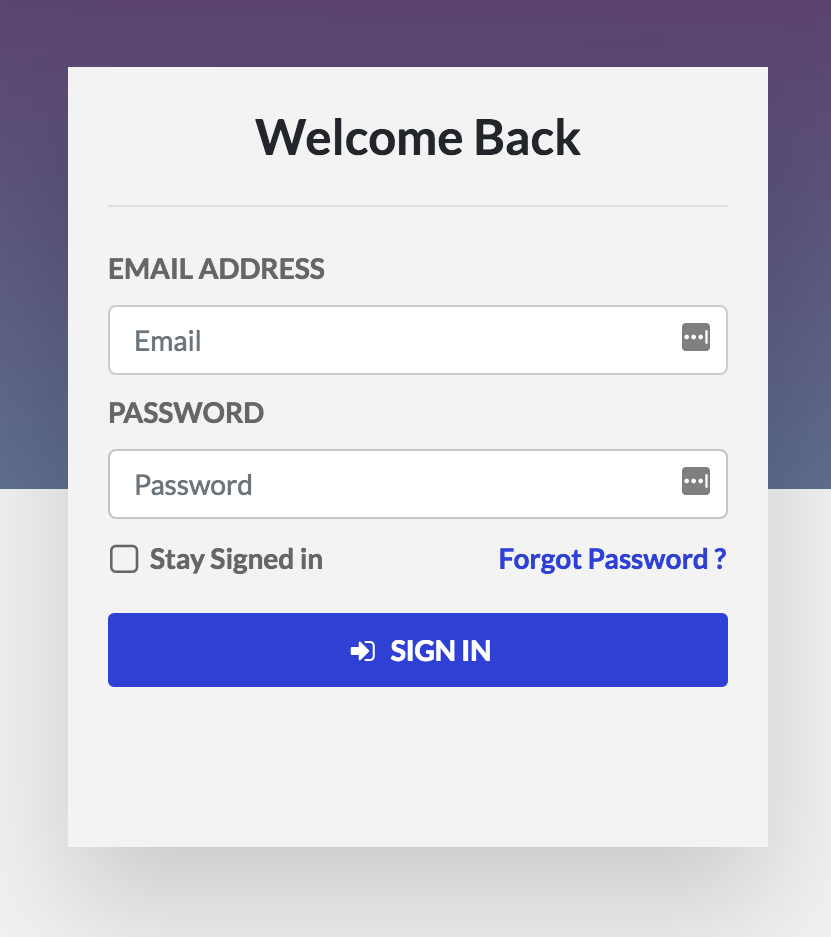
\includegraphics[width=.8\linewidth]{images/test_case_1/original_page_anon_cropped.png}
		\label{fig:original_page_anon}
	\end{subfigure}%
	\begin{subfigure}{.5\textwidth}
		\centering
		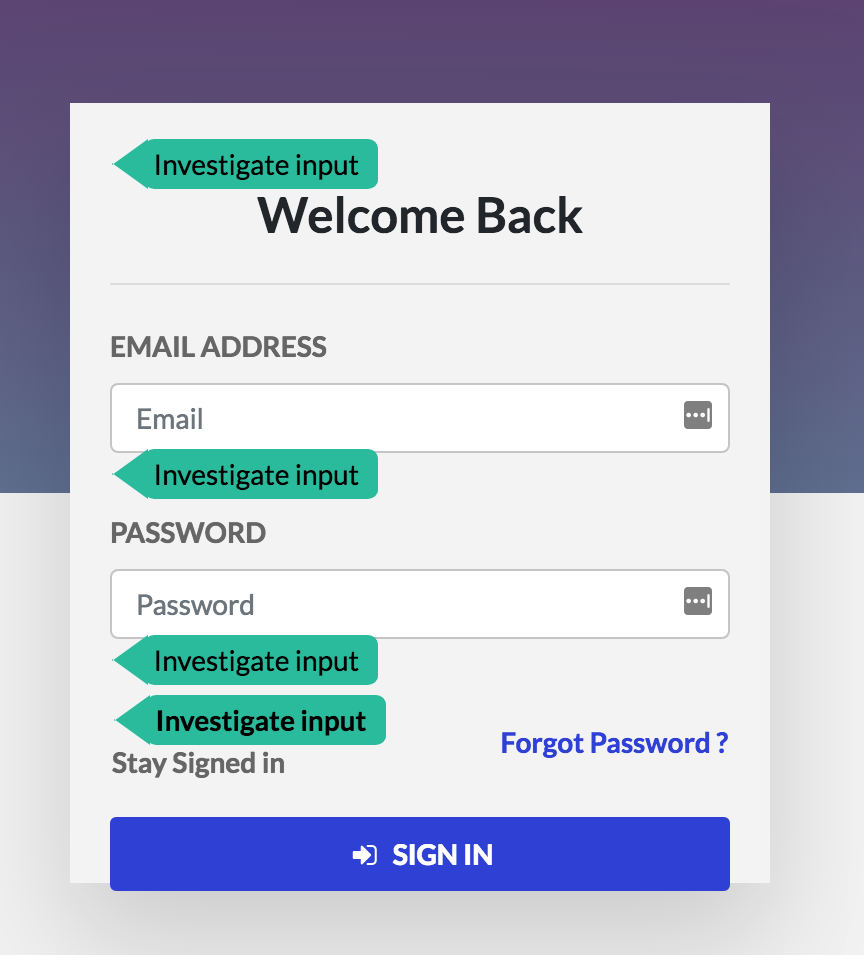
\includegraphics[width=.8\linewidth]{images/test_case_1/recommendations_anon_cropped.png}
		\label{fig:recommendations_anon}
	\end{subfigure}
	\caption{Here we see the website form before and after having the \textit{Recommendations} setting enabled. We see that it highlights both normal inputs in the form, as well as a hidden input, shown by the \textit{Investigate Form} button floating above the "Welcome Back" text.}
	\label{fig:vuln_page}
\end{figure} 

We decide to "investigate" the email input further - by clicking the button it automatically submits the form using an attack from those preprogrammed in the extension. The attack we submit at this time is an XSS attempt by trying to inject an image whose \texttt{onerror} property is triggered due to a faulty image source. Attempting this injection gives us the output shown in Figure \ref{fig:trigger_point}. \\

\begin{figure}[h!]
	\centering
	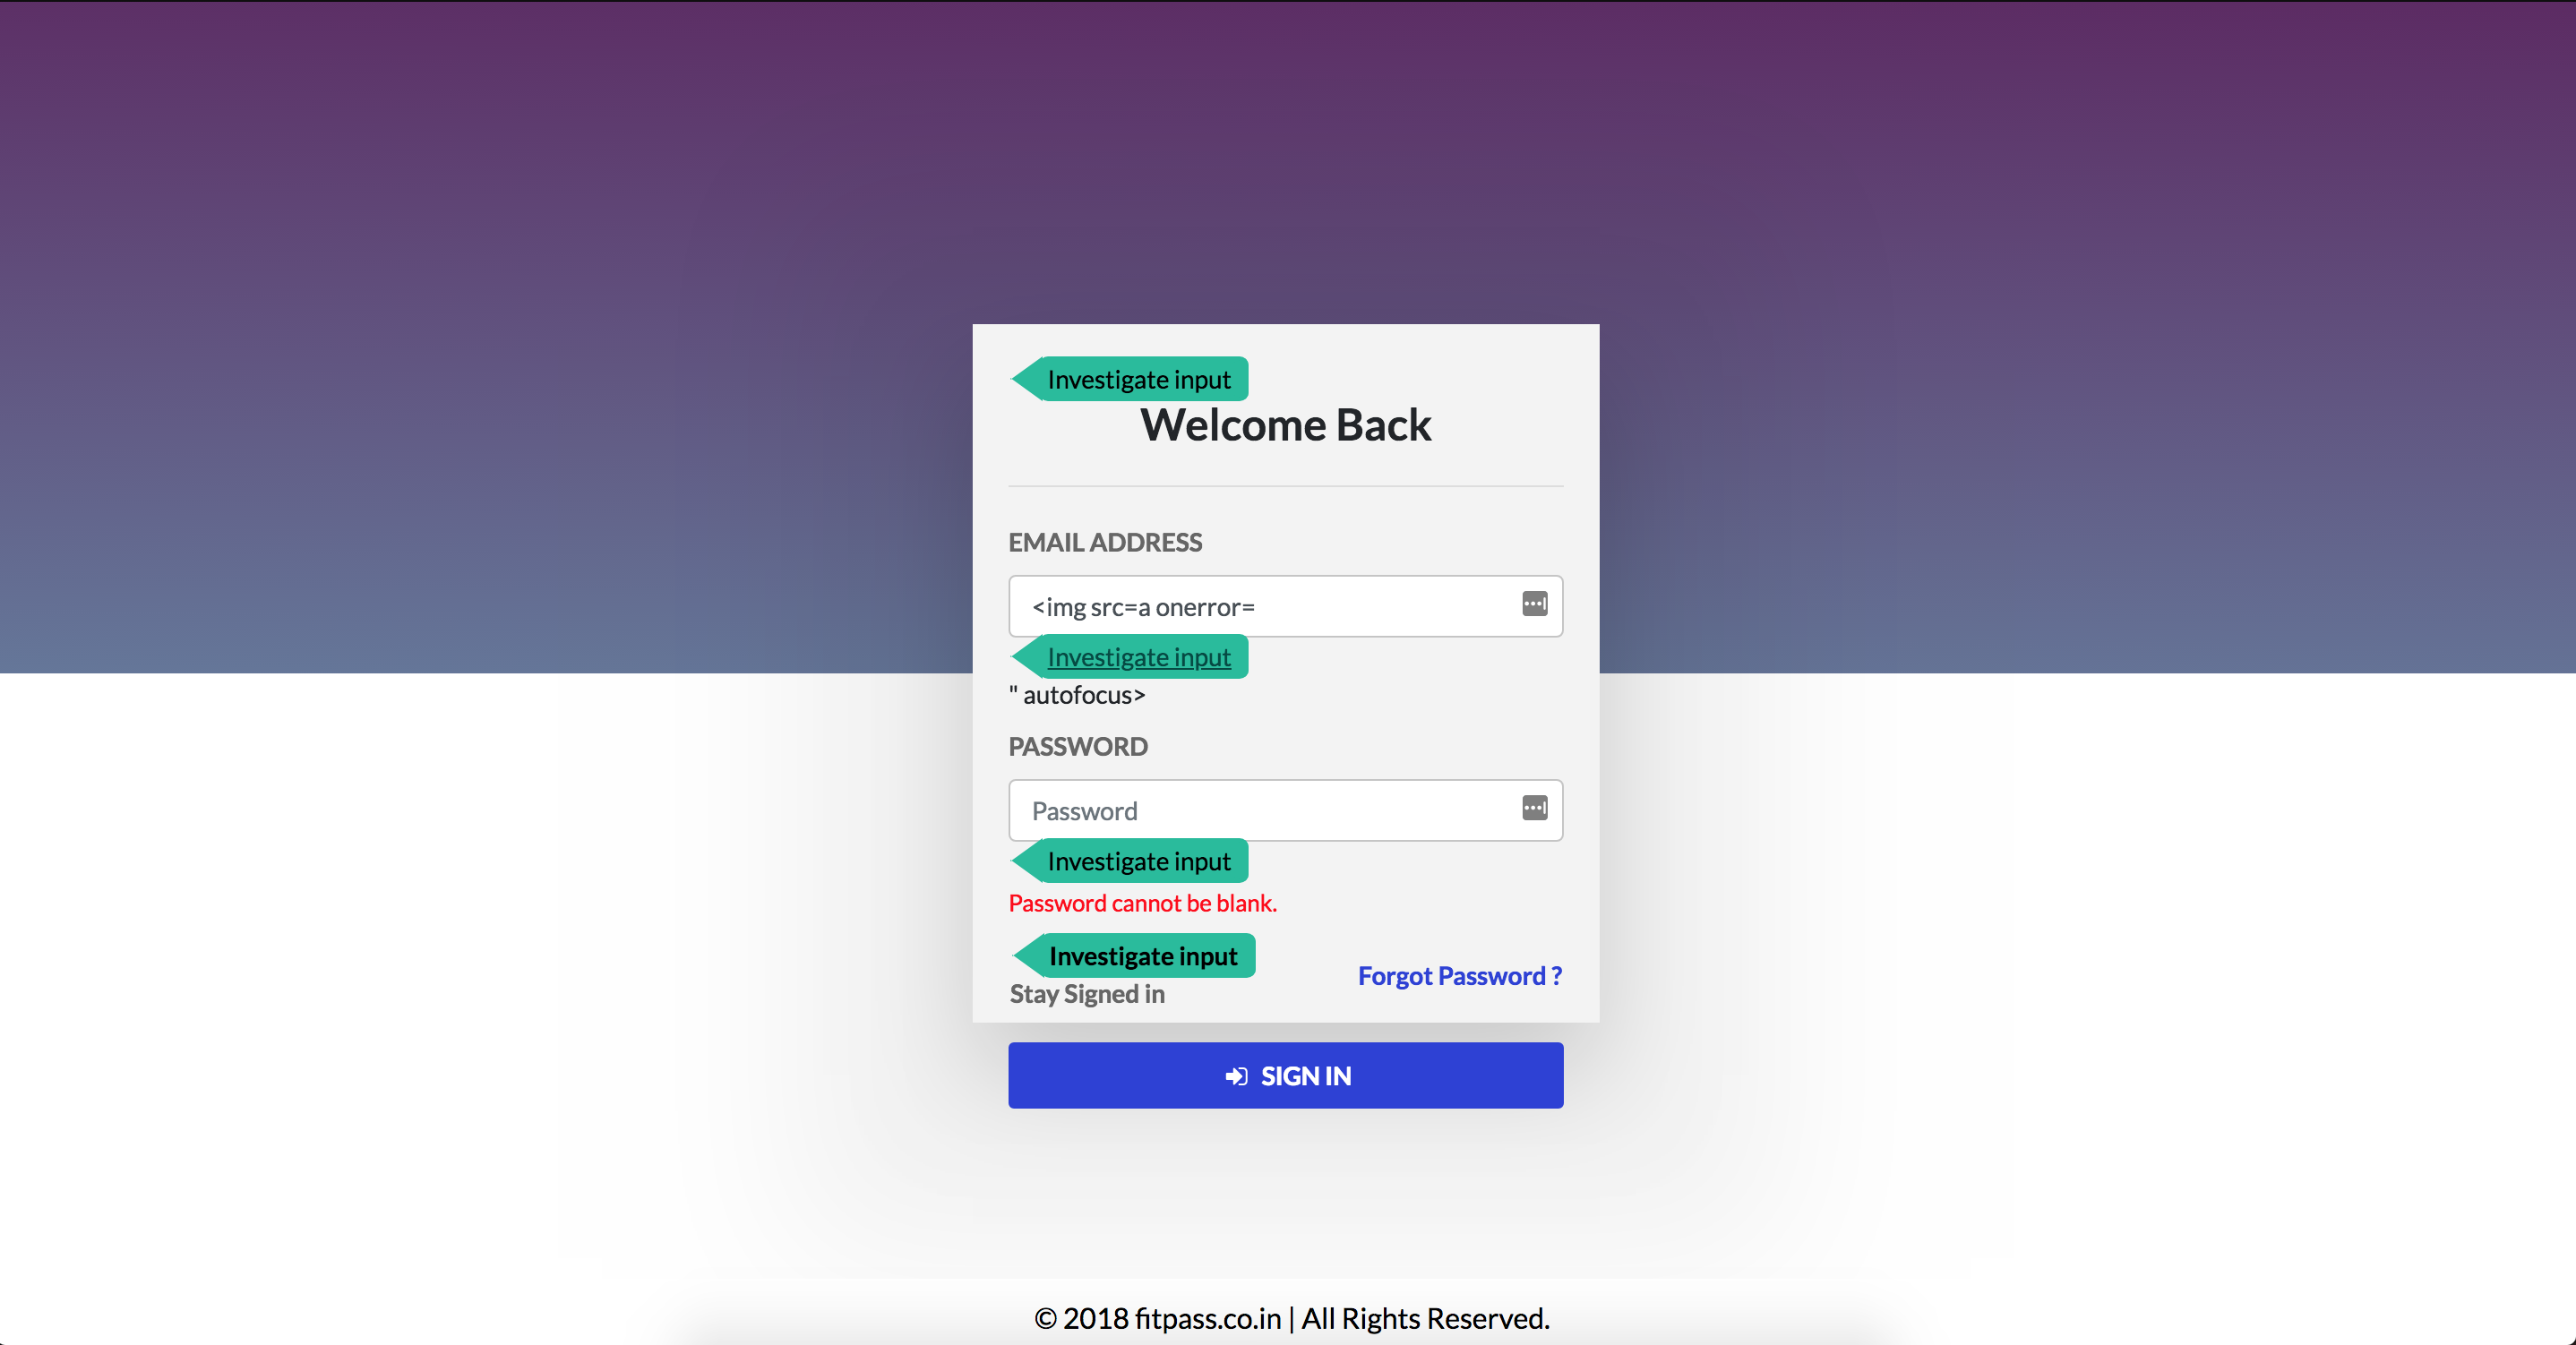
\includegraphics[width=0.75\textwidth]{images/test_case_1/trigger_point_anon.png}
	\caption{Here the form returns an error with a warning saying that the \textit{Password can't be blank}. However, this is not the interesting behaviour - we instead notice the presence of the following text after the Email address input: \texttt{" autofocus>}. This wasn't there before, and is not part of the attack.}
	\label{fig:trigger_point}
\end{figure}

This behaviour is interesting because the form has now added the text \texttt{" autofocus>} onto the form. This text was not previously in the login form; neither before or after adding the recommendations onto the page, so it must have been added as a result of submitting the attack on the form. To confirm this, we can check the source code of the page before and after the attack. 

\begin{figure}[h!]
	\centering
	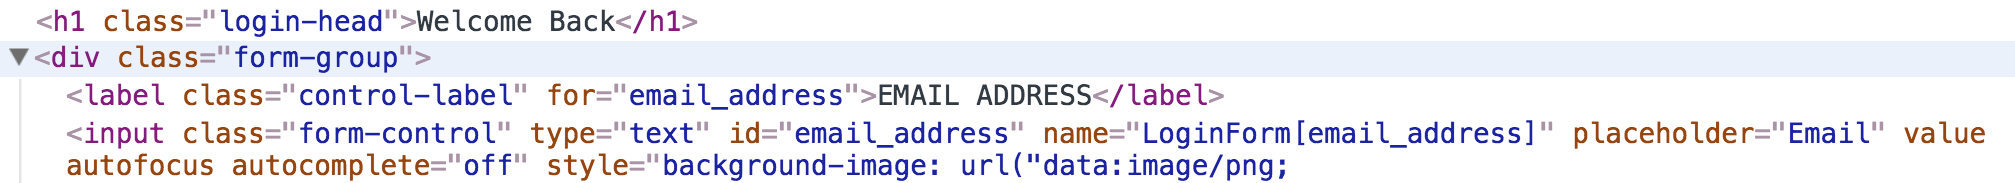
\includegraphics[width=\linewidth]{images/test_case_1/src_code_before.png}
	\caption{The source code of the login form before adding the recommendations or submitting an attack.}
	\label{fig:src_code_before}
\end{figure}

\begin{figure}[h!]
	\centering
	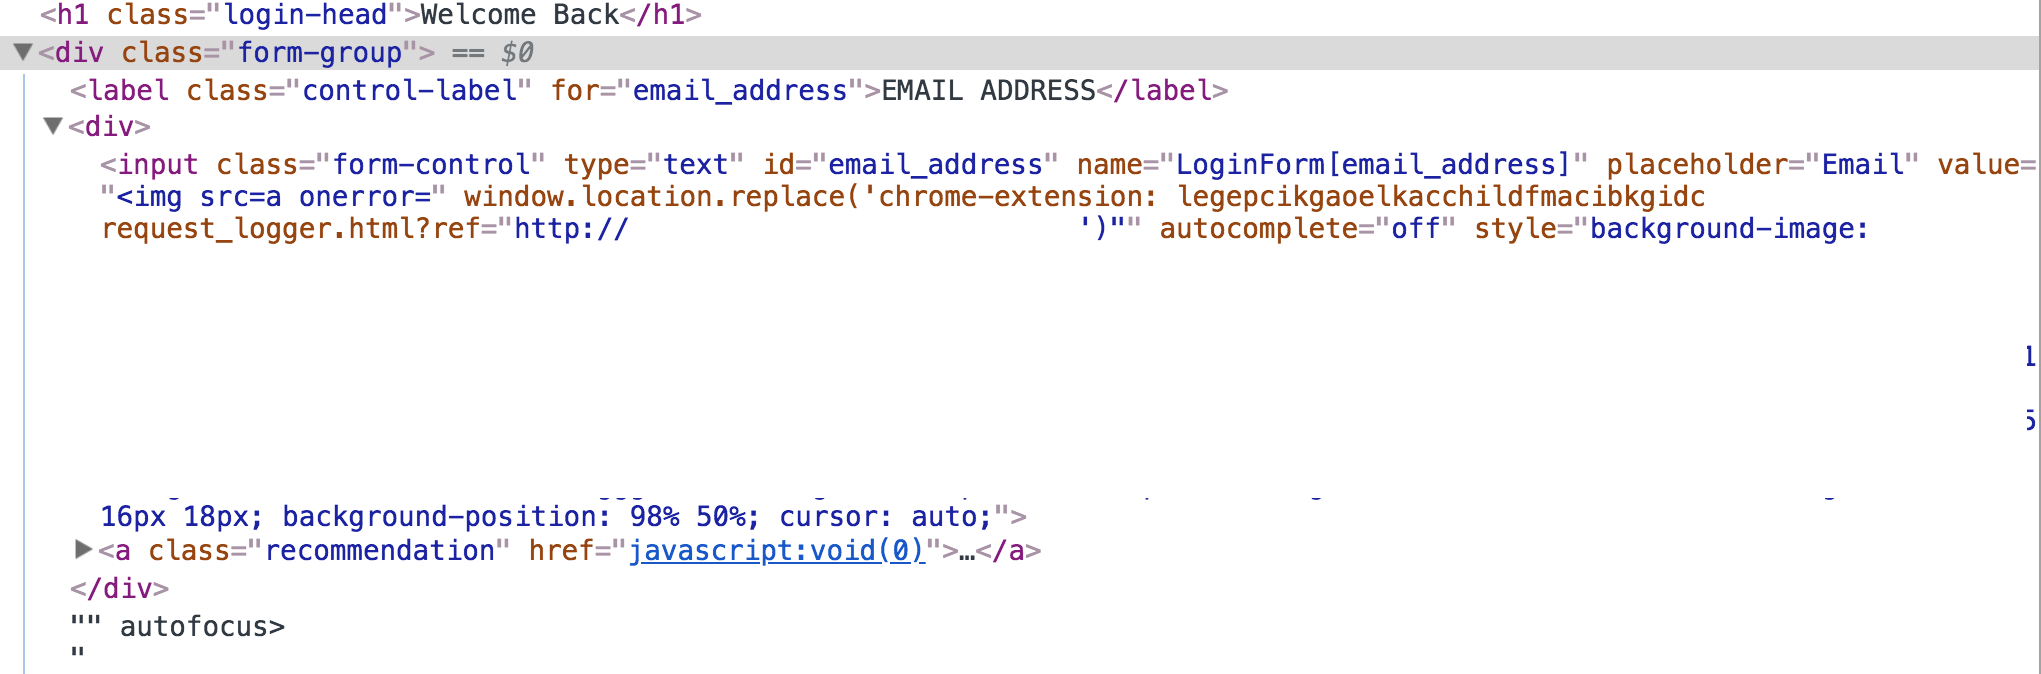
\includegraphics[width=\linewidth]{images/test_case_1/src_code_after.png}
	\caption{The source code of the login form after executing the attack (edited for anonymity).}
	\label{fig:src_code_after}	
\end{figure} 

Comparing the page source code before and after submitting the attack shows that before the attack, the \texttt{autofocus} attribute was immediately after the \texttt{value} attribute of the \texttt{email} input. The \texttt{value} attribute had no prior setting. We know that upon submission of a form, the \texttt{value} attribute of an input is changed to whatever the user has submitted. In this case, that value contained the \texttt{"} character. What seems to have happened is that the browser adds the quote characters to encapsulate the incoming value for this attribute (as they were not present before), but because that value contains quote characters of its own, these are not escaped, and thus cause a shift in attributes in the form input. That explains why we see the shift of the \texttt{autofocus} attribute towards the bottom of the code section in Figure \ref{fig:src_code_after}. \\

Armed with this knowledge, we can now play the role of a potential attacker and experiment with different inputs to try and generate an exploit. Before proceeding and potentially wasting time on attempting exploits that may not work, we enable Passive Mode and have a quick look at whether using this form tells us anything about the headers being set on the page. Figure \ref{fig:passive_analysis} only alerts us to the lack of a \texttt{Content-Security-Policy}. \\

\begin{figure}[h!]
	\centering
	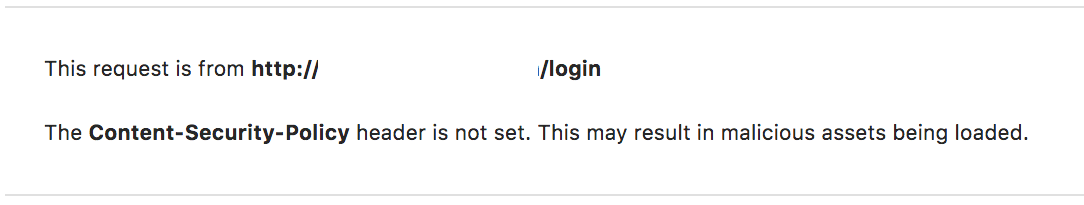
\includegraphics[width=\linewidth]{images/test_case_1/passive_analysis.png}
	\caption{Analysing the website using the Passive Mode of the extension reveals that of the security headers, only the \texttt{Content-Security-Policy} header hasn't been set. }
	\label{fig:passive_analysis}	
\end{figure} 

This saves a website pentester some time - they may skip attempting to craft an XSS exploit as an example because the \texttt{X-XSS-Protection} header has already been set, which makes this difficult unless they know specific ways to bypass browser XSS protection. This for example means that we cannot make use of inline Javascript attributes (such as \texttt{onclick}), but does not prevent us from using other HTML attributes. We can attempt to craft a form which looks similar to the present one, but with a different result from submission - we try and trick a user into downloading a file from an external source. \\

To start this, we want to introduce our own elements into the form, but we know we can't directly remove elements from that form, since we don't have access to Javascript to remove this. We can however shift the contents of the page, just as we have inadvertently done with the \texttt{autofocus} attribute. Following this principle, we try and shift the current contents of the form as far down the page as we can. We do this by injecting prematurely closing DOM tags in the email input. We try the following attack:

\begin{center}
	\texttt{"></form></section>}
\end{center}

This produces the webpage as shown in Figure \ref{fig:attack_form_1}. That figure shows what is immediately visible to the user. However, if the user were to scroll down in the page, they would see the remaining contents of the form, which have simply been displaced further down the page - as seen in Figure \ref{fig:scroll_attack_1}.

\begin{figure}[h!]
	\centering
	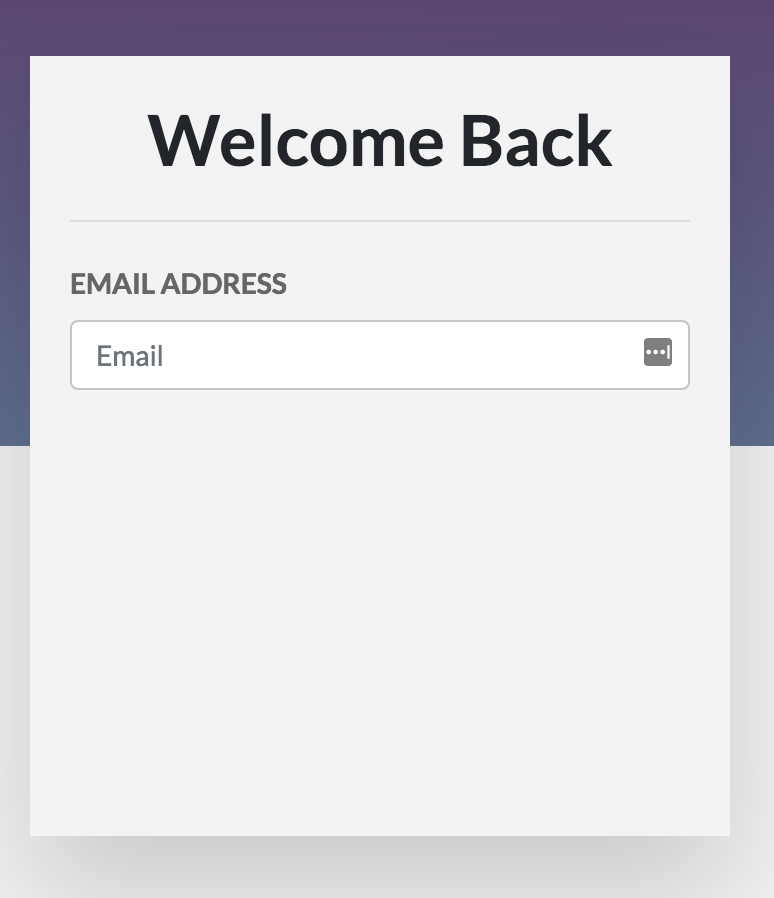
\includegraphics[width=0.6\linewidth]{images/test_case_1/attack_form_1.png}
	\caption{This is the resulting page from prematurely closing DOM tags. }
	\label{fig:attack_form_1}	
\end{figure} 


\begin{figure}[h!]
	\centering
	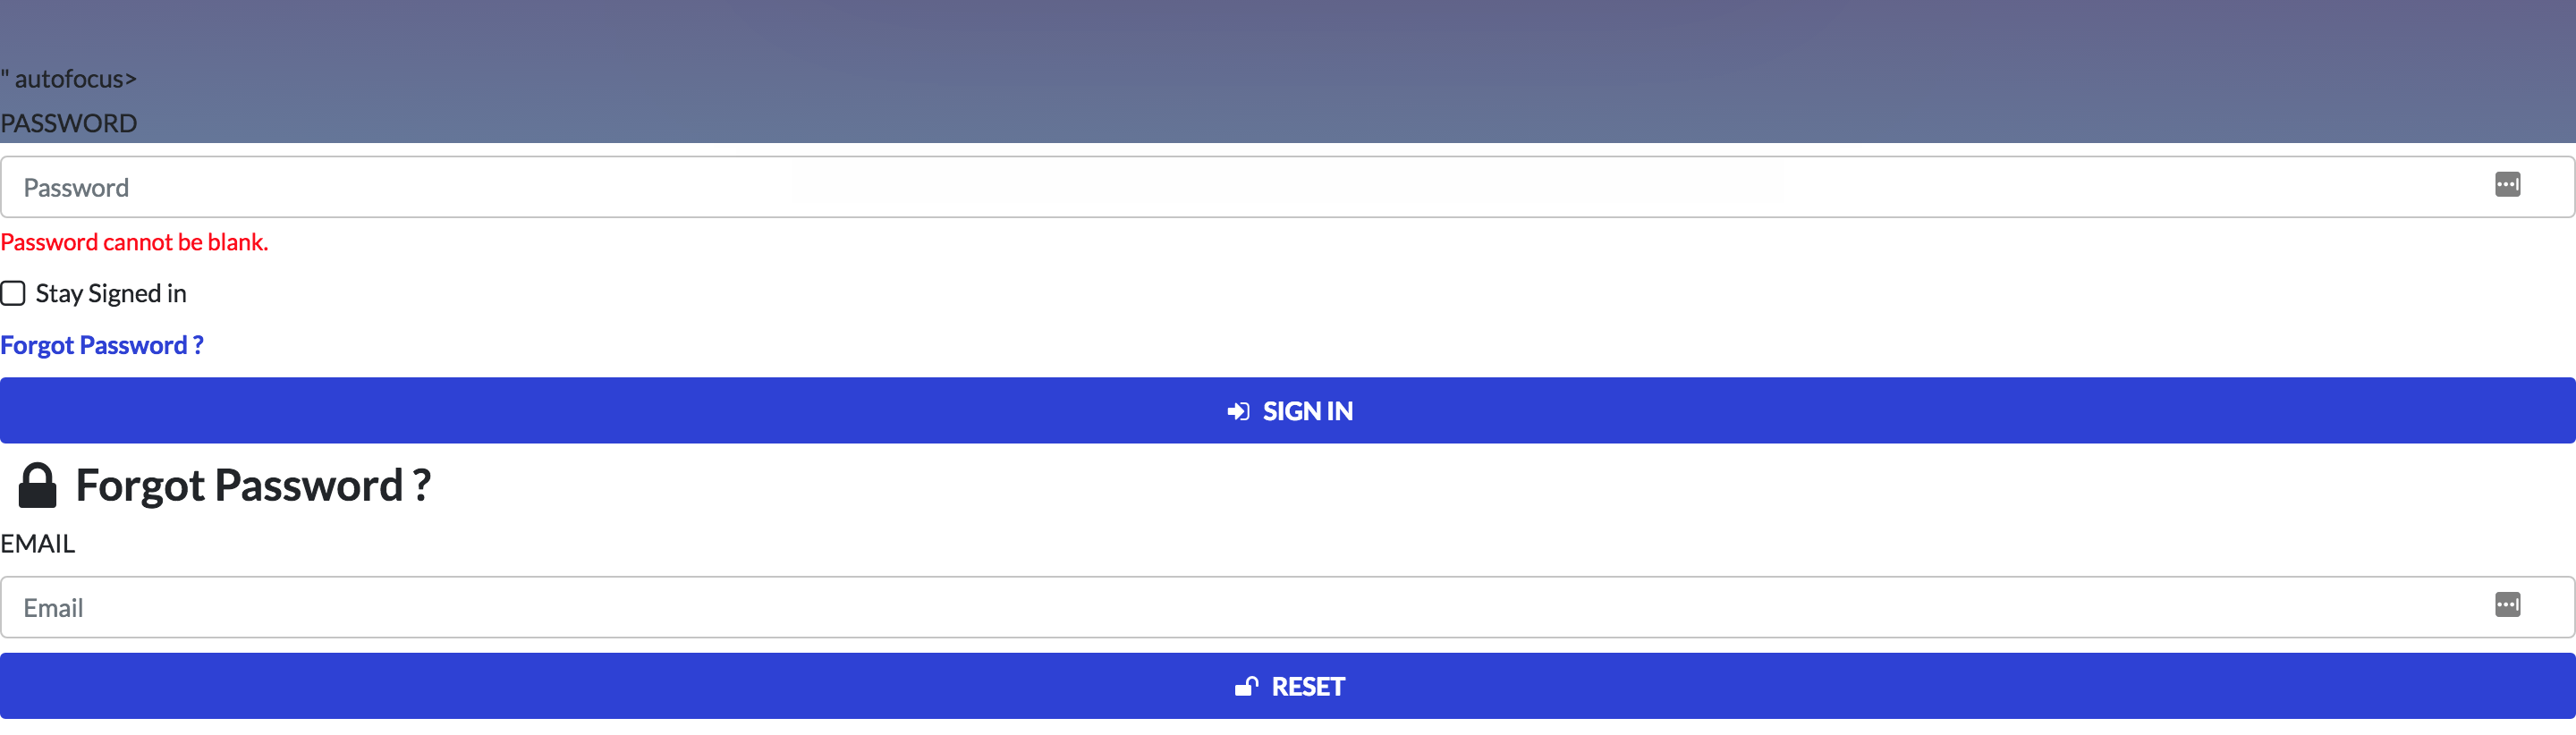
\includegraphics[width=\linewidth]{images/test_case_1/scroll_attack_1.png}
	\caption{Scrolling down the page reveals the "missing" contents of the form to submit.}
	\label{fig:scroll_attack_1}	
\end{figure} 

Now that we have figured out how to make it seem as if the contents of the form are broken, we can add in our own elements to this form. Since our goal is to make the user inadvertently download a file, we simply need the user to click somewhere with a link to that file. It is tempting to attempt to steal their password and email address by making the form submit to a website we control, thus including these details in the request. However, changing the \texttt{action} attribute of the form to a value we control would be picked up by the browser's XSS auditor, and thus disabled. To fulfill our goal, we thus want to inject an anchor (\texttt{<a>}) tag to replace the \textit{Submit} button on the form. In order to start the download of the file, we make the \texttt{href} attribute of this tag link to a webpage where this file is hosted. For the purposes of this example, we have prepared a file to be hosted at a website we control, with a file extension we know Chrome automatically downloads, \texttt{.dmg}(some file extensions such as \texttt{.pdf} open up special browser features). Since the attacks are being executed on a macOS, this file type is considered an executable, and is downloaded automatically. Obviously, the contents of this file are harmless, we are only showing a proof-of-concept in terms of exploits. \\



%http://studios.fitpass.co.in/login






















%
\chapter{Experimentation}
	

\section{Intended functionality}
In order to be able to perform the functionality as proposed above, the project should be able to demonstrate the following characteristics:

\begin{enumerate}
	\item \textbf{Recommendation system} - The browser extension must be able to passively analyse web traffic and produce visual cues that indicate to the user that it has detected a potential vulnerability. From these, the user should be able to initiate a session where they can try and detect a vulnerability.
	
	\item \textbf{Passive mode} - The extension is designed to eventually be able to take active steps to detect a vulnerability. It's undesirable for the extension to do this if these active steps may infringe terms of service of using the application. Active steps in this context encompass any automated features of the extension that behave on behalf of the user, such as sending web requests, filling out forms etc. Passive steps include the extension reading and analysing web traffic explicitly performed by the user, including suggesting recommendations based on the results of this analysis (the extension should not be liable for any user behaviour that may infringe terms of service, so if passive mode is not enabled, the user has no excuses so as to say they were not aware that the tool infringed these terms without their knowledge). Therefore, the extension must have a clearly visible toggle such that the user can enable or disable active vulnerability detection steps. 
	
	\item \textbf{Action Replay} - As described before, the tool should be able to record user inputs in a targeted domain from when they initiate a vulnerability scanning session until the user declares it is finished. The tool should then be able to replicate these steps automatically, while changing and fuzzing inputs when doing so. Each replication should attempt to reset the web application state inbetween tries to accurately represent fuzzing user input from the state they defined as a starting point for that particular scan.
	
	\item \textbf{Educational functionality} - In order to be able to meet its purpose of being educational to users who don't necessarily run the extension with prior web security knowledge, the tool should have a limited library of plaintext knowledge to explain different vulnerability types, how these may be detected, and suggestions on how to exploit them thereafter. Snippets of this knowledge may be presented under the recommendations shown to users when using the extension. A more detailed explanation may be provided in the pop-up page that appears when the user clicks on the extension icon in the browser.
\end{enumerate}


\section{Metrics of success}

To appropriately judge the success of the extension, we must have some quantifiable metrics, described below

\begin{enumerate}
	\item \textbf{Time to vulnerability} - As mentioned in \ref{limitations}, measuring the total time taken to perform a scan in this human driven context is unfair; the tool does not set a boundary on total scans unlike an automated scanner does. Measuring time taken is however a useful metric, so in order to not completely circumvent using time, another more appropriate metric is suggested - \emph{time to vulnerability}. This will be measured as the total number of seconds taken from the moment a scan is initiated (the user clicks the visual cue given by the tool), until the scan is finished. A scan may finish under two circumstances: a vulnerability has been successfully reported or detected (this may happen at the first attempt by the user, or at a later try when the tool has fuzzed some inputs during the 'action replay' phase), or when the tool reports it could not find a vulnerability. These 2 conditions are bounded in terms of possible time taken, allowing the total time to be measured.
	
	\item \textbf{Interaction volume} - A metric that is sometimes found when evaluating automated scanners  is that of bytes sent and received by the application \cite{stateOfArtAutomatedBlackBoxWebAppVulnTesting}. This quantifies the impact the tool has when stressing the website by fuzzing inputs. The smaller this metric is, the more efficiently the tool is performing its job, by detecting vulnerabilities with fewer web requests sent.
	
	\item \textbf{Number of replays needed} - A similar metric to interaction volume, this number measures how many 'replays' are required by the tool to successfully detect a vulnerability. Both of these metrics measure the efficiency of the tool in detecting vulnerabilities, but this metric more accurately tests the efficiency of the fuzzing engine provided by the tool. Ideally, the tool uses the inputs which are known to work with higher success rates first, and the more esoteric fuzzes would come last, when there is already a decreased likelihood of them working anyway. It also encourages the tool to only include meaningful and relevant fuzzing techniques per vulnerability type, otherwise the tool \emph{could} theoretically fuzz forever. The fewer number of replays needed by the tool in order to find a vulnerability, the better it is performing.
	
%	\item \textbf{Recommendation to vulnerability conversion rate} - An automated scanner is often measured in terms of how many false positives it shows, because it is expected to either positively or negatively declare the existence of a vulnerability. This would be an unfair means of benchmarking this extension - 
\end{enumerate}


\section{Experiments}


\subsection{Test benches}
In order to test my tool during development, it is not necessary to build a vulnerable web application from scratch. Not only would this be time consuming (beyond the purposes of building a tool to exploit such an application), it would also bias the ensuing development of the extension so that it is tailored to successfully detect every injected vulnerability in the web application. Fortunately, there already exist tools dedicated to this purpose. \\

As previously mentioned, DVWA is a vulnerable web application written in PHP, using MySQL for database interactions \cite{dvwaSite}. This application contains a good selection of predefined vulnerabilities to test against:
\begin{multicols}{3}
\begin{itemize}
\item Brute Force Login
\item Command Execution
\item CSRF
\item File Inclusion
\item SQL Injection
\item Upload Vulnerability
\item XSS	
\end{itemize}
\end{multicols}

Another existing tool is WebGoat \cite{webgoatIntro, webgoatGithub}, supported by OWASP. This is an actively supported project by the open source community, and also contains a healthy amount of potential vulnerabilities for developers to test against:

\begin{multicols}{3}
\begin{itemize}
\item 	Access Control Flaws
\item 	AJAX Security
\item 	Authentication Flaws
\item 	Buffer Overflows
\item 	Code Quality
\item 	Concurrency
\item 	Cross-Site Scripting (XSS)
\item 	Improper Error Handling
\item 	Injection Flaws
\item 	Denial of Service
\item 	Insecure Communication
\item 	Insecure Configuration
\item 	Insecure Storage
\item 	Malicious Execution
\item 	Parameter Tampering
\item 	Session Management Flaws
\item 	Web Services
\item 	Admin Functions
\end{itemize}
\end{multicols}

Similarly to the above, there exist more testing tools of this kind, such as WackoPicko \cite{wackoPickoGithub} and HacmeBank \cite{hacmeBankMcAfee}. A more extensive list of existing applications of this kind has been produced by OWASP \cite{owaspVulnerableWebAppsList}. For the purposes of the experiments in this project, I will test against DVWA, WebGoat and WackoPicko, in order, as needed per vulnerability. This provides a good variety of implementations of vulnerabilities to test against; if the tool successfully finds the targeted vulnerabilities in these applications then it is likely to do well in other contexts.

\subsection{Test methodology}
The main method of testing my extension is to pit my extension against other existing automated vulnerability scanners. Some potential candidate scanners include \emph{OWASP ZAP} \cite{owaspZapPage}, \emph{w3af} \cite{w3af} and \emph{burpsuite} \cite{burpSuitePage}. All the scanners will analyse the aforementioned vulnerable applications used in testing. To avoid the case where the produced extension overfits its scanning model to the test vulnerable applications, this experiment will include more applications from the OWASP vulnerable web apps list \cite{owaspVulnerableWebAppsList}, not previously used in testing. \\

Since the browser extension makes use of user input, it is important to test the application with people of different security backgrounds. This relies on adequate classification in this group by the person undertaking the test. There will be 3 proposed categories of user experience when testing the tool; advanced, intermediate and beginner. An advanced user is expected to be well versed in web security, and have had prior experience in diagnosing (perhaps exploiting) vulnerabilities. An intermediate user may be someone getting to grips with this area, perhaps a student who is only now learning about these concepts, but hasn't \emph{necessarily} got experience in detecting or exploiting vulnerabilities. Beginner users are expected to be web savvy, people who are acquainted with using browsers and web applications, but are not necessarily interested or knowledgeable in web security. It is hoped that enough data is gathered to be able to have at least 5 unique people per suggested user group - it may be particularly hard to find advanced users that are willing to test the tool, whereas users who fit the other categories should be much easier to find. \\

To quantify how well the tool performs its job, the success rates of all 3 groups will be analysed when using the extension to find vulnerabilities. A very successful implementation of the project will have made it easy for non-experts to detect vulnerabilities, meaning that results from the beginner group would not vary very much from those in the intermediate and advanced groups using the tool. Therefore, inter-group vulnerability detection success rates will be analysed. From these success rates, it may be possible to extrapolate data on how educational the project was to users in the beginner and intermediate groups. This data could be further backed up by an additional quiz on whether the user has understood the type of vulnerability they detected, and whether they understand the ramifications of doing so by providing an example of a potential exploit they might design as a result. \\

Additionally, comparing each group success rate to the success rates of each of the automated scanners is useful to be able to validate the claim that a user driven, semi-automated approach is advantageous. This should be done within the context of what vulnerabilities the extension is able to detect - if an automated scanner can find more types of vulnerabilities than the ones the extension has been designed to find, then these will not be counted in the results. For a fair comparison in that aspect, it is assumed that with more development time, the extension may be developed further to be able to identify another type of vulnerability. \\

Another means of testing the success of the application would be to put it to test against real world applications. By activating the described passive mode as needed, and browsing web application domains, it is possible that a user of the extension finds vulnerabilities in the target application. Should this happen, it would be a great validating factor for the success of the tool.


\chapter{Evaluation}


In this section we will take a retrospective look at the tool and its achievements. We observe some benchmarks ran against competitors as well as measure how well Gentoo has performed given the expected pre-requisites as set out earlier in this thesis. We will also attempt to given a qualitative evaluation of how well it has performed, given initial user feedback (beyond the quantitative analysis).

\section{Metrics of success}

To appropriately judge the success of the extension, we must have some quantifiable metrics, described below

\begin{enumerate}
	\item \textbf{Time to vulnerability} - As mentioned in \ref{limitations}, measuring the total time taken to perform a scan in this human driven context is unfair; the tool does not set a boundary on total scans unlike an automated scanner does. Measuring time taken is however a useful metric, so in order to not completely circumvent using time, another more appropriate metric is suggested - \emph{time to vulnerability}. This will be measured as the total number of seconds taken from the moment a scan is initiated (the user clicks the visual cue given by the tool), until the scan is finished. A scan may finish under two circumstances: a vulnerability has been successfully reported or detected (this may happen at the first attempt by the user, or at a later try when the tool has fuzzed some inputs during the Action Replay phase), or when the tool reports it could not find a vulnerability. These 2 conditions are bounded in terms of possible time taken, allowing the total time to be measured.
	
	\item \textbf{Interaction volume} - A metric that is sometimes found when evaluating automated scanners  is that of bytes sent and received by the application \cite{stateOfArtAutomatedBlackBoxWebAppVulnTesting}. This quantifies the impact the tool has when stressing the website by fuzzing inputs. The smaller this metric is, the more efficiently the tool is performing its job, by detecting vulnerabilities with fewer web requests sent.
	
	\item \textbf{Number of replays needed} - A similar metric to interaction volume, this number measures how many 'replays' are required by the tool to successfully detect a vulnerability. Both of these metrics measure the efficiency of the tool in detecting vulnerabilities, but this metric more accurately tests the efficiency of the fuzzing engine provided by the tool. Ideally, the tool uses the inputs which are known to work with higher success rates first, and the more esoteric fuzzes would come last, when there is already a decreased likelihood of them working anyway. It also encourages the tool to only include meaningful and relevant fuzzing techniques per vulnerability type, otherwise the tool \emph{could} theoretically fuzz forever. The fewer number of replays needed by the tool in order to find a vulnerability, the better it is performing.
	
	%	\item \textbf{Recommendation to vulnerability conversion rate} - An automated scanner is often measured in terms of how many false positives it shows, because it is expected to either positively or negatively declare the existence of a vulnerability. This would be an unfair means of benchmarking this extension - 
\end{enumerate}


\section{Experiments}


\subsection{Test benches}
In order to test our tool during development, it was not immediately necessary to build a vulnerable web application from scratch. A much more bare bones approach was taken with the Test Harness, by building a page which presented the basic features of the vulnerabilities we were interested in exploiting. This provided a good balance of effort into producing a custom testing page with having a vulnerable application we control entirely.
 %Not only would this be time consuming (beyond the purposes of building a tool to exploit such an application), it would also bias the ensuing development of the extension so that it is tailored to successfully detect every injected vulnerability in the web application.
  Fortunately, there already exist tools dedicated to this purpose. \\

As previously mentioned, DVWA is a vulnerable web application written in PHP, using MySQL for database interactions \cite{dvwaSite}. This application contains a good selection of predefined vulnerabilities to test against:
\begin{multicols}{3}
	\begin{itemize}
		\item Brute Force Login
		\item Command Execution
		\item CSRF
		\item File Inclusion
		\item SQL Injection
		\item Upload Vulnerability
		\item XSS	
	\end{itemize}
\end{multicols}

Another existing tool is WebGoat \cite{webgoatIntro, webgoatGithub}, supported by OWASP. This is an actively supported project by the open source community, and also contains a healthy amount of potential vulnerabilities for developers to test against:

\begin{multicols}{3}
	\begin{itemize}
		\item 	Access Control Flaws
		\item 	AJAX Security
		\item 	Authentication Flaws
		\item 	Buffer Overflows
		\item 	Code Quality
		\item 	Concurrency
		\item 	XSS
		\item 	Improper Error Handling
		\item 	Injection Flaws
		\item 	Denial of Service
		\item 	Insecure Communication
		\item 	Insecure Configuration
		\item 	Insecure Storage
		\item 	Malicious Execution
		\item 	Parameter Tampering
		\item 	Session Management Flaws
		\item 	Web Services
		\item 	Admin Functions
	\end{itemize}
\end{multicols}

Similarly to the above, there exist more testing tools of this kind, such as WackoPicko \cite{wackoPickoGithub} and HacmeBank \cite{hacmeBankMcAfee}. A more extensive list of existing applications of this kind has been produced by OWASP \cite{owaspVulnerableWebAppsList}. For the purposes of the experiments in this project, we will test against DVWA, WebGoat and WackoPicko, in order, as needed per vulnerability. This provides a good variety of implementations of vulnerabilities to test against; if the tool successfully finds the targeted vulnerabilities in these applications then it is likely to do well in other contexts.

\subsection{Test methodology}
The main method of testing the extension is to pit Gentoo against other existing automated vulnerability scanners. Some potential candidate scanners include \emph{OWASP ZAP} \cite{owaspZapPage}, \emph{w3af} \cite{w3af} and \emph{burpsuite} \cite{burpSuitePage}. All the scanners will analyse the aforementioned vulnerable applications used in testing. \\
% To avoid the case where the produced extension overfits its scanning model to the test vulnerable applications, this experiment will include more applications from the OWASP vulnerable web apps list \cite{owaspVulnerableWebAppsList}, not previously used in testing. \\

Since Gentoo makes use of user input, it is important to test the application with people of different security backgrounds. This relies on adequate classification in this group by the person undertaking the test. There will be 3 proposed categories of user experience when testing the tool; advanced, intermediate and beginner. An advanced user is expected to be well versed in web security, and have had prior experience in diagnosing (perhaps exploiting) vulnerabilities. An intermediate user may be someone getting to grips with this area, perhaps a student who is only now learning about these concepts, but hasn't \emph{necessarily} got experience in detecting or exploiting vulnerabilities. Beginner users are expected to be web savvy, people who are acquainted with using browsers and web applications, but are not necessarily interested or knowledgeable in web security. It is hoped that enough data is gathered to be able to have at least 5 unique people per suggested user group - it may be particularly hard to find advanced users that are willing to test the tool, whereas users who fit the other categories should be much easier to find. \\

To quantify how well the tool performs its job, the success rates of all 3 groups will be analysed when using the extension to find vulnerabilities. A very successful implementation of the project will have made it easy for non-experts to detect vulnerabilities, meaning that results from the beginner group would not vary very much from those in the intermediate and advanced groups using the tool. Therefore, inter-group vulnerability detection success rates will be analysed. From these success rates, it may be possible to extrapolate data on how educational the project was to users in the beginner and intermediate groups. This data could be further backed up by an additional quiz on whether the user has understood the type of vulnerability they detected, and whether they understand the ramifications of doing so by providing an example of a potential exploit they might design as a result. \\

Additionally, comparing each group success rate to the success rates of each of the automated scanners is useful to be able to validate the claim that a user driven, semi-automated approach is advantageous. This should be done within the context of what vulnerabilities the extension is able to detect - if an automated scanner can find more types of vulnerabilities than the ones the extension has been designed to find, then these will not be counted in the results. For a fair comparison in that aspect, it is assumed that with more development time, the extension may be developed further to be able to identify another type of vulnerability. \\

Another means of testing the success of the application would be to put it to test against real world applications. By activating the described passive mode as needed, and browsing web application domains, it is possible that a user of the extension finds vulnerabilities in the target application. Should this happen, it would be a great validating factor for the success of the tool.


\section{Benchmark analysis}

We now compare and analyse Gentoo's performance against other tools when scanning vulnerable web applications. We will be using OWASP's Zed Attack Proxy Project (\textit{ZAP}), and the Web Application Attack and Audit Framework (\textit{w3af}) as points of comparison - both of these are open source web scanners. In order to ensure a fair basis for comparing these tools, we used a virtual machine running the \textit{Kali} Linux distribution\footnote{ Kali version 3.26.2. The virtual machine was allocated 3.9GB memory, using an Intel i7-4980HQ at 2.8GHz (2 cores)} and installed each tool in this VM. \\

 As part of setting up these benchmarks (which were mostly geared towards finding XSS vulnerabilities as per Gentoo's current functionality), it was also necessary to use a proxy to disable the browser's XSS Auditor. Since the benchmarks are comprised of web applications with intentionally vulnerable functionalities, we want to observe this functionality without the extra protections added by the browser. For this purpose, we use BurpSuite's proxying feature to capture requests and disable the \texttt{X-XSS-Protection} header (should it be present, Figure \ref{fig:burp_xss_disabled}). We enable its use in Chrome by linking it with \textit{ProxySwitchOmega} \footnote{ ProxySwitchOmega is a Google Chrome extension to enable request proxying: https://goo.gl/iFSJvH.}. Obviously, in a real website setting, we would not control this setting, making it more difficult for Gentoo to actively exploit XSS vulnerabilities. \\

\begin{figure}[h]
	\centering
	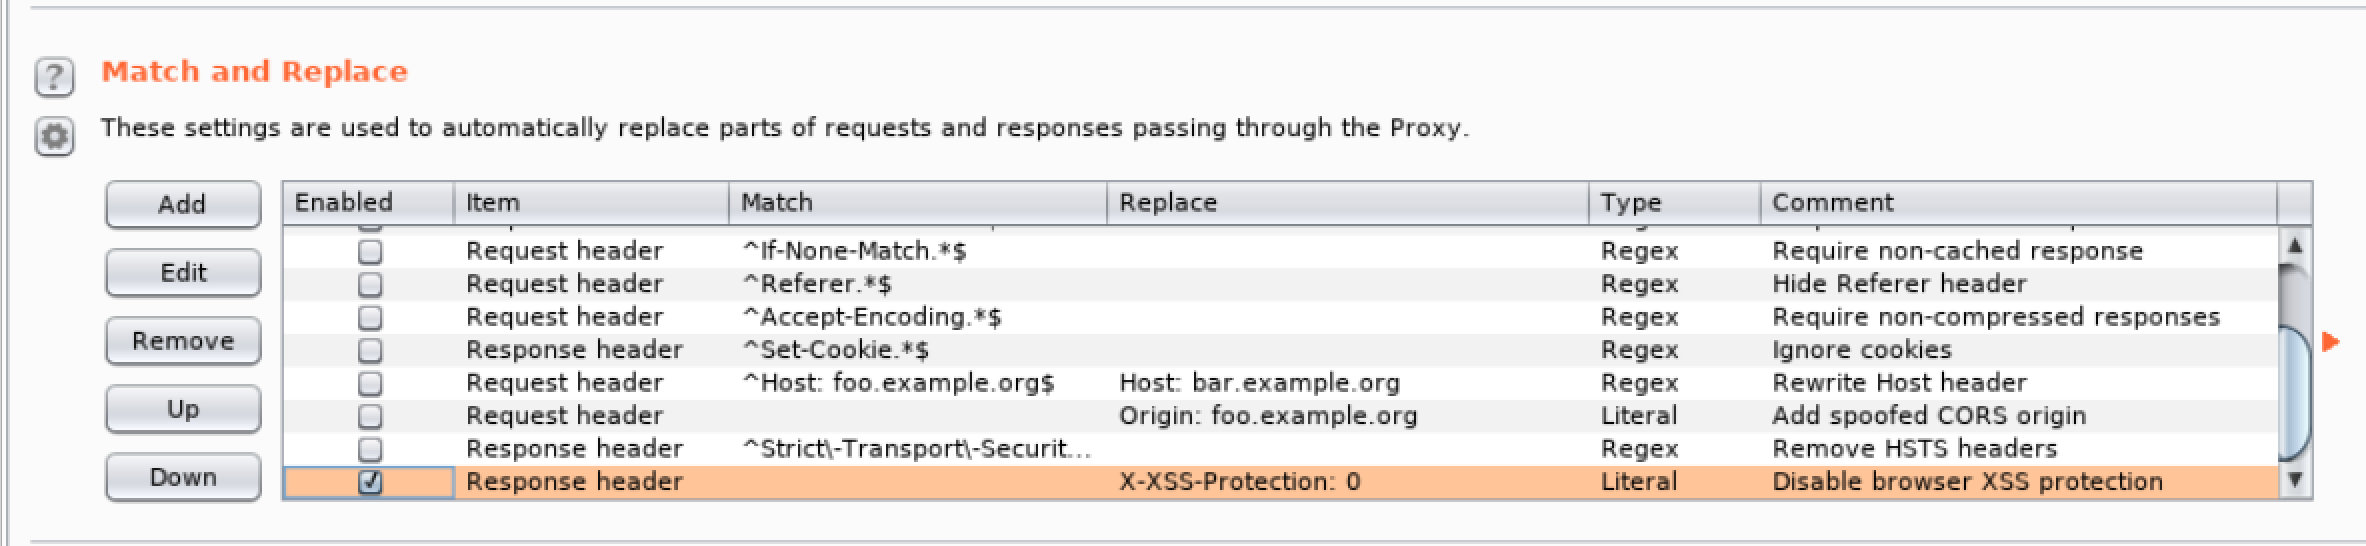
\includegraphics[width=\textwidth]{images/evaluation/burp_xss_disabled.png}
	\caption{Any request passed to Gentoo or the other tools is stripped of the \texttt{X-XSS-Protection} header, allowing for accurate XSS detection.}
	\label{fig:burp_xss_disabled}
\end{figure}

As explained before, we will be extracting 3 key metrics: \textit{Time to Vulnerability}, \textit{Interaction Volume} and \textit{Number of Attacks needed}. \textit{Time to vulnerability} is measured as the time from the moment the scan is initiated until the first 'vulnerability' is detected by the application (irrespective of whether this is the vulnerability we are specifically looking for or not - we will explain the reasoning for this later). \textit{Interaction Volume} is measured as the total number of bytes used in the scan by the tool. \textit{Number of attacks needed} measures how many requests a tool had to make before finding its first vulnerability in the scan (as a proportion to how many requests it made in the scan overall). \\ 

In order to extract data for the purposes of these experiments, we use console logging in Gentoo to acquire accurate timestamps for key events in a scan. For the other tools, we use the provided reporting and exporting functionalities by each tool and analyse the outputs of these to acquire the necessary data. \\

\subsection{Test Harness}

Firstly, we benchmarked the tools against the produced Test Harness. We ran Gentoo using the Action Replay functionality to detect the XSS vulnerabilities present in this page, and subsequently used the Passive Mode to scan the headers in the Test Harness. For ZAP, we used the \textit{Launch Browser} feature to crawl the page, and subsequently attacked it with all selected input vectors. We used the \textit{full\_audit} profile provided by w3af to perform the corresponding scan. \\

\begin{table}[h]
	
{\rowcolors{3}{green!24}{white}

	   \captionsetup{justification=centering}
	
	\caption{Running the tools against the Test Harness. The * by the \textit{Time to Vulnerability} column indicates the desired vulnerability (XSS) was not detected. The \textit{Attacks to Vuln / Total attacks} shows how many attacks were needed by the tool to reach the first vulnerability alert, relative to the total number of attacks in the scan.}
		\label{table:test_harness_benchmarks}
\begin{tabular}{ |p{4cm}||p{1.4cm}|p{1.4cm}|p{1.6cm}|p{2cm}|p{2cm}| }
	\hline
	\multicolumn{6}{|c|}{\textbf{Test Harness Benchmarks}} \\ [0.5ex]
	\hline \hline 
	Tool Being Tested& Time To Vulnerability & Total Scan Time & Interaction Volume & Attacks to Vuln / Total Attacks & \% of scan to 1st vuln \\
	\hline
	Gentoo (XSS detection)    & 9.6s      & 15.8s    & 32KB & 10/27 &37\% \\
	Gentoo (Header Analysis) & 50ms    &  3.0s    & 4KB&  1/4 &25\%\\
	ZAP                                   & 5.6s (*) & 7.8s      &  1.31MB &1621/2140 &76\%\\ 
	w3af                                 & 7.9s  (*) & 136.2s & 950KB & 71/1126 &6.3\%\\
	\hline
\end{tabular}
} \\
\end{table}

Table \ref{table:test_harness_benchmarks} shows how each tool performed when measured up against the aforementioned metrics. For the XSS detection in Gentoo, we intentionally measure the time taken by a human to interact with the extension to analyse the outputs produced. The scan begins once the Action Replay recording begins, which means a form input must be manually submitted, the Action Replay button clicked on the new page, and each of the resulting attacks inspected for vulnerabilities. The scan is considered to be finished once the last successful attack has been registered as an observable output in the extension (at the same time the extension badge icon turns to an exclamation mark (\textbf{!})), or, in the absence of a vulnerability, once the user has finished inspecting the attacks. \\

In this case, 2 separate attacks were successful in triggering an XSS vulnerability during the extension's scan. It took the user a relatively short time to come to this conclusion, as the scan only took around 16 seconds. This seems especially successful when compared to the other automated results - ZAP's scan was about half the time, whilst w3af's was unusually long, and neither of these seemed to have correctly found the XSS flaw on the page. The order in which attacks were performed seemed to be good, with the first vulnerability being reported when the Gentoo scan was only about 37\% of the way through. In comparison to the other tools, it is clear both by the number of requests and the interaction volume that Gentoo did this with a significantly lower number of requests. This could be due to overfitting and creator's bias however, as the Test Harness was heavily used alongside the development of Gentoo. We will bear this in mind as we look at other vulnerable pages shortly.  \\

When producing this data, it became evident that comparing Gentoo to these tools on a basis of whether they had found a specific vulnerability on an application seemed unfair. As it stands, our extension is very focused on finding a given vulnerability, and if set up correctly, seems to provide good feedback on said vulnerability. However, ZAP and w3af are stand-alone implementations designed to run without user interaction, and as such, will scan the entire web-application in a non-discriminatory way when it comes to selecting vulnerabilities - anything of use is flagged up for the final report. Thus, although we set up these tests in a manner such that Gentoo \textit{should} find a vulnerability it has been designed to catch, we will not hold it against the results of the other 2 should they find other useful information along the way. \\

In the benchmark above (Table \ref{table:test_harness_benchmarks}), neither ZAP nor w3af reported an XSS vulnerability for the Test Harness. This is perhaps a little odd, as the page containing this vulnerability conforms to the minimum requirements for a Reflected XSS. However, since it is a \textit{very} simple page, it could be supposed that the page is not complex enough for the filters being used by the other scanners to correctly classify it as vulnerable to XSS. \\

Nonetheless, all 3 of the tools produced warnings when analysing the application headers. With the exception of w3af, the tools seem to clearly indicate whether the results are being passively obtained or not. However, when observing the scan, the speed at which the alerts in w3af are produced seems to indicate that internally, these are still acquired passively from web requests. \\

\begin{table}[h]
	
	{\rowcolors{3}{green!24}{white}

		\captionsetup{justification=centering}
		
		\caption{The alerts produced by the different tools when analysing the Test Harness}
		\label{table:test_harness_alerts}
		\begin{tabular}{ |p{7cm}|>{\centering\arraybackslash}m{2cm} |>{\centering\arraybackslash}m{2cm} |>{\centering\arraybackslash}m{2cm}| }
			\hline
			\multicolumn{4}{|c|}{\textbf{Test Harness passive alerts}} \\ [0.5ex]
			\hline \hline 
			Alert Type & Gentoo & ZAP & w3af \\
			\hline
			X-Frame-Options (Clickjacking) & X & X & X \\
			X-XSS-Protection & X & X & \\
			X-Content-Type-Options& X & X & \\
			Content-Security-Policy & X & & \\
			Referrer-Policy & X & & \\
			Strict-Transport-Security & X  & & \\
			Server Header Exposed & & & X\\
			DNS Wildcard config & & & X \\
			Too many HTTP methods allowed & & & X\\
			
			\hline
		\end{tabular}
	} \\
\end{table}

In Table \ref{table:test_harness_alerts}, we see that all of tools can agree that clickjacking is a big enough concern that the \texttt{X-Frame-Options} header should be set. We will ignore the alerts for the missing \texttt{X-XSS-Options} header because this is by design as previously explained, although it is interesting to note that w3af did not report this missing header in its scans. Some of the uniquely reported headers by Gentoo are also more recent additions - both the \texttt{Content-Security-Policy} and the \texttt{Referrer-Policy} are newer headers. As for the last 4 on the Table, these alerts are mostly suggestions rather than warnings - these are flagged up by Gentoo and w3af, but do not necessarily indicate weaknesses. They are nonetheless useful in the \textit{information gathering} phase for any pentester, and shouldn't be readily ignored. \\ 

\subsection{DVWA}

We now proceed to look at how these tools perform at a more homogenous level by benchmarking them against a third-party produced application. \\
\begin{table}[h]
	
	{\rowcolors{3}{green!24}{white}

		\captionsetup{justification=centering}		
		\caption{Running the tools against DVWA.}
		\label{table:dvwa_benchmarks}
		\begin{tabular}{ |p{4cm}||p{1.4cm}|p{1.4cm}|p{1.6cm}|p{2cm}|p{2cm}| }
			\hline
			\multicolumn{6}{|c|}{\textbf{DVWA Benchmarks}} \\ [0.5ex]
			\hline \hline 
			Tool Being Tested& Time To Vulnerability & Total Scan Time & Interaction Volume & Attacks to Vuln / Total Attacks & \% of scan to 1st vuln \\
			\hline
			Gentoo (Reflected XSS)    & 6.6s      & 9.4s    &   66.3KB          & 4/15 & 27 \% \\
			Gentoo (Persisted XSS)    &  -- & 5.3s & 80.6KB & 13/13 & 100 \% \\
			Gentoo (Header Analysis) & 27ms    &  3.0s    & 17.9KB   &  2/5 & 40\%\\
			ZAP                                  & 2.6s & 66.6s     &  65.79MB & 3852/22995& 16.7\%\\ 
			w3af                                 & -- & -- & -- & -- &-- \\
			\hline
		\end{tabular}
	} \\
\end{table}

Once again, the results for the Gentoo XSS detection seem promising - the scan duration in DVWA is still very reasonable, even accounting for human interaction delays. The attack order is also effective, as the first confirmed vulnerability is found after just a quarter of the attacks are performed. However, Gentoo's search for a persisted XSS failed in the page containing that vulnerability. None of the attacks forged against this page worked - for a very simple reason. The Persistent XSS vulnerability in DVWA involves submitting a \texttt{textarea} - a form input that isn't designated by the \texttt{input} HTML tag. This is an oversight in Gentoo's page injection logic, as \texttt{textarea}'s are perfectly valid inputs to submit. However, this concern had not been addressed before this benchmark, negatively affecting Gentoo's evaluation. \\

 Unfortunately, we weren't able to configure w3af to successfully scan DVWA. w3af does possess authentication enabled scans and crawls as a feature, but we were unable to configure it in such a way that it could log into DVWA as a user as part of its crawl. The resulting crawl was very debilitated as a result - only very few resources that were not hidden behind the login form were accessible, and so we could not count this towards w3af's overall performance. \\
 
 In this benchmark, ZAP has performed very well. It executed close to 23 thousand requests in just over a minute, and detected its first serious vulnerability in only 2.6 seconds. This is an example where automated scanners can boast of their alacrity - all the while performing over 1500x more requests than Gentoo, it still found a vulnerability faster than a human could. \\

Table \ref{table:dvwa_alerts} highlights this further. During this time, ZAP has not only detected a Reflected XSS, but also Persisted XSS and other severe vulnerabilities - Path Traversals and SQL injections. At this point it's worth mentioning that Gentoo's passive mode, as with the Test Harness, has detected and warned the user about the same set of headers as ZAP has, although Gentoo's header selection is more extensive than that of ZAP's. Both also found that the valuable \texttt{PHPSESSID} cookie should have probably been set with the \texttt{httpOnly} flag to maximise session security. In this respect, both scanners have done well - ZAP has used the extra time of its scan to find important and relevant vulnerabilities. Its scan time is still over 5 times the duration of the combined Gentoo scans, so this success should almost be expected in an application such as DVWA, which is brimming with vulnerabilities.



\begin{table}[h]
	
	{\rowcolors{3}{green!24}{white}
		
		\captionsetup{justification=centering}
		
		\caption{The alerts \& warnings produced by the different tools when analysing DVWA. Those with ** are real, dangerous vulnerabilities found in DVWA}
		\label{table:dvwa_alerts}
		\begin{tabular}{ |p{7cm}|>{\centering\arraybackslash}m{2cm} |>{\centering\arraybackslash}m{2cm} |>{\centering\arraybackslash}m{2cm}| }
			\hline
			\multicolumn{4}{|c|}{\textbf{DVWA alerts}} \\ [0.5ex]
			\hline \hline 
			Alert Type & Gentoo & ZAP & w3af \\
			\hline
			XSS (Reflected) ** & X & X & --\\
			XSS (Persistent) ** &  & X & --\\
			Path Traversal ** &  & X & --\\
			SQL Injection **& & X & --\\
			X-Frame-Options (Clickjacking) & X & X & -- \\
			X-XSS-Protection & X & X & --\\
			X-Content-Type-Options& X & X &-- \\
			Content-Security-Policy & X & &-- \\
			Referrer-Policy & X & & --\\
			Strict-Transport-Security & X  & & --\\
			PHPSESSID Cookie Insecure Flags & X & X & -- \\
			\hline
		\end{tabular}
	} \\
\end{table}



\subsection{WebGoat}

Moving on, we now observe how each of the tools performs when scanning WebGoat, OWASP's deliberately insecure application designed to teach security lessons. Unfortunately, we still couldn't configure w3af's authentication module to sign into WebGoat. As a result, it could still not perform any relevant scanning besides passive header analysis for alerts and warnings, and as such, it is not included in the following results. \\

 Surprisingly, Gentoo is unable to perform the Action Replay on this application. Although it can visually start a scan, under these circumstances, the \texttt{DevTools} script cannot identify the WebGoat page to be the active tab, resulting in an exception which does not allow the Action Replay algorithm to complete. As a result, only Gentoo's Passive mode worked as normal, acquiring weak header and cookie data as before. ZAP managed to complete another full application scan; using it's \textit{Launch Browser} feature, we were able to log into a user profile as part of the scan, and emulate and crawl the application while this browser was open. Once we are happy with the extent of the crawling performed, we can then tell ZAP to perform several attacks based off of this information. \\

\begin{table}[h]
	
	{\rowcolors{3}{green!24}{White}
		\captionsetup{justification=centering}		
		\caption{Running the tools against WebGoat}
		\label{table:webgoat_benchmarks}
		\begin{tabular}{ |p{4cm}||p{1.4cm}|p{1.4cm}|p{1.6cm}|p{2cm}|p{2cm}| }
			\hline
			\multicolumn{6}{|c|}{\textbf{WebGoat Benchmarks}} \\ [0.5ex]
			\hline \hline 
			Tool Being Tested& Time To Vulnerability & Total Scan Time & Interaction Volume & Attacks to Vuln / Total Attacks & \% of scan to 1st vuln \\
			\hline
			Gentoo (XSS detection)    & --     & --    &   --          & -- & -- \\
			Gentoo (Header Analysis) &  3.2s   & 6.2s   & 1.3MB   & 1/3 & 33.3\%\\
			ZAP                                   & 12.9s &  48.5s   & 68.0MB  & 1213/4437 & 27.3\%\\ 
			w3af                                 & -- & -- & -- & -- & -- \\
			\hline
		\end{tabular}
	} \\
\end{table}


Gentoo's header analysis is again very terse, as it picks up very few requests in order to analyse the necessary headers - the first vulnerability is found in the first of these. The interaction volume this time however is significantly larger, as WebGoat generates a lot more data per request than the other applications thus far. In the meantime, ZAP remains a consistent opponent by delivering a hefty scan in a reasonable time - under a minute. This is enough time to reel in 4 serious vulnerabilities, which the other tools have missed out on by lack of compatibility. Gentoo's header analysis still picks up on valuable session ID cookies and alerts to their lack of security, as does ZAP. 

\begin{table}[h]
	
	{\rowcolors{3}{green!24}{white}
		
		\captionsetup{justification=centering}
		
		\caption{The alerts \& warnings produced by the different tools when analysing WebGoat. Those with ** are dangerous vulnerabilities found in WebGoat}
		\label{table:webgoat_alerts}
		\begin{tabular}{ |p{7cm}|>{\centering\arraybackslash}m{2cm} |>{\centering\arraybackslash}m{2cm} |>{\centering\arraybackslash}m{2cm}| }
			\hline
			\multicolumn{4}{|c|}{\textbf{WebGoat alerts}} \\ [0.5ex]
			\hline \hline 
			Alert Type & Gentoo & ZAP & w3af \\
			\hline
			XSS (Reflected) ** & -- & X & --\\	
			SQL Injection **& -- & X & --\\
			XSS (Reflected in JSON Response) ** & -- & X & -- \\
			Parameter Tampering **& -- & X & --\\
			X-XSS-Protection & X & X & --\\
			Content-Security-Policy & X & &-- \\
			Referrer-Policy & X & & --\\
			Strict-Transport-Security & X  & & --\\
			JSESSID Cookie Insecure Flags & X & X & -- \\
			PHPSESSID Cookie Insecure Flags & X & X & -- \\
			\hline
		\end{tabular}
	} \\
\end{table}


\subsection{WackoPicko}

WackoPicko is our final benchmark in which Gentoo will be compared against the other tools. This time, Gentoo has no problem scanning the application for an XSS vulnerability using Action Replay. WackoPicko hides some of its behaviour behind a user login, however, it has sufficient crawlable content outside of this form such that w3af produces relevant output from its scan without having to be configured to sign into the application. \\

\begin{table}[h]
	
	{\rowcolors{3}{green!24}{white}
		\captionsetup{justification=centering}		
		\caption{Running the tools against WackoPicko.}
		\label{table:wackopicko_benchmarks}
		\begin{tabular}{ |p{4cm}||p{1.4cm}|p{1.4cm}|p{1.6cm}|p{2cm}|p{2cm}| }
			\hline
			\multicolumn{6}{|c|}{\textbf{WackoPicko Benchmarks}} \\ [0.5ex]
			\hline \hline 
			Tool Being Tested& Time To Vulnerability & Total Scan Time & Interaction Volume & Attacks to Vuln / Total Attacks & \% of scan to 1st vuln \\
			\hline
			Gentoo (XSS detection)    &   11.6s   &  17.8s   &  52.0KB           & 1/24 & 4.1\% \\
			Gentoo (Header Analysis) &  51ms &  3.1s  &  1.6KB  & 3/7 & 42.9 \%\\
			ZAP                                   & 53s &  184.3s   & 254.4MB & 10854/46301 & 23.4\%\\ 
			w3af                                 & 458ms & 498s & 7.0MB & 2/8279 & 0.02\% \\
			\hline
		\end{tabular}
	} \\
\end{table}

From Table \ref{table:wackopicko_benchmarks}, we once again see that Gentoo's XSS detection works very effectively; despite taking into account human interaction, the user is able to efficiently detect an XSS vulnerability within seconds. Across all of the benchmarks, Gentoo has remained very succint, with a few well directed requests that are then able to detect a vulnerability. This time, ZAP delivers a much larger scan, making over 46 thousand requests in 3 minutes. w3af also has more to work with this time, so after a lengthy 8 minute scan, it has made 7MB of interactions over 8279 requests - but it surprisingly finds its first vulnerability within the second request it made, making this benchmark run (relatively) the fastest to obtain a vulnerability as a function of the size of the scan. \\


\begin{table}[h]
	
	{\rowcolors{3}{green!24}{white}
		
		\captionsetup{justification=centering}
		
		\caption{The alerts \& warnings produced by the different tools when analysing WackoPicko. Those with * are serious vulnerabilities, not present in Wackopicko, whereas those with ** are real, dangerous vulnerabilities found in WackoPicko}
		\label{table:wackopicko_alerts}
		\begin{tabular}{ |p{7cm}|>{\centering\arraybackslash}m{2cm} |>{\centering\arraybackslash}m{2cm} |>{\centering\arraybackslash}m{2cm}| }
			\hline
			\multicolumn{4}{|c|}{\textbf{WackoPicko alerts}} \\ [0.5ex]
			\hline \hline 
			Alert Type & Gentoo & ZAP & w3af \\
			\hline
			XSS (Reflected) ** & X & X & X\\
			XSS (Persistent) ** &  & X & \\
			Path Traversal ** &  & X & X\\
			SQL Injection **& & X & X\\
			Parameter Tampering ** &  & X & \\
			CSRF * & & & X \\
			Guessable Credentials (Weak Auth) ** & & & X \\
			X-Frame-Options (Clickjacking) & X & X & X \\
			X-XSS-Protection & X & X & \\
			X-Content-Type-Options& X & X & \\
			Content-Security-Policy & X & &\\
			Referrer-Policy & X & & \\
			Strict-Transport-Security & X  & & \\
			PHPSESSID Cookie Insecure Flags & X & X &  \\
			\hline
		\end{tabular}
	} \\
\end{table}

As we see from Table \ref{table:wackopicko_alerts}, Gentoo has once again performed its duty and found the Reflected XSS vulnerability, as well as the usual list of weak security headers and session cookies. This is consistent with its previous behaviours, demonstrating it can perform an accurate scan whilst making judicious use of the requests it makes. However, we cannot ignore the payoffs for spending a longer time in scanning as shown by ZAP and w3af - both of these detected the Reflected XSS as well as other serious vulnerabilities. Notably, the CSRF vulnerability is not actually reported by the creators of WackoPicko as a present vulnerability, so we assume this is a false-positive result from the w3af scan. Nonetheless, the remainder of these results  provide very valuable insights to a penetration tester. \\

\subsection{Cross evaluation}

At this stage, we would benefit from a deeper analysis across the aforementioned figures to ascertain a comparison between the tools and their expected performances. We start by looking at the \textit{Time to Vulnerability} that each tool has shown when scanning the different vulnerable web applications. Figure \ref{fig:time_to_vuln} shows how each tool has performed against one another in their respective scans. \\ 

It becomes apparent that Gentoo's figures are the most stable when compared across the different web application scans. The XSS focused attacks seem to range anywhere between between 5 to 15 seconds. It is important to remember however that these scans are still dependent on human interaction - depending on the experience of the user who is using the Action Replay mechanism to collect data, this scan \textit{could} take a lot longer, as the user (or their machine) may be overwhelmed with the amount of windows opened to carry out each attack. The speed in these numbers probably suffers from a bias of knowing how to use Gentoo from a creator's perspective. Nonetheless, it is promising to see that the lower boundary for the time taken in this scan is competitive when pitted against the other scanners. \\

\begin{figure}[h]
	\centering
	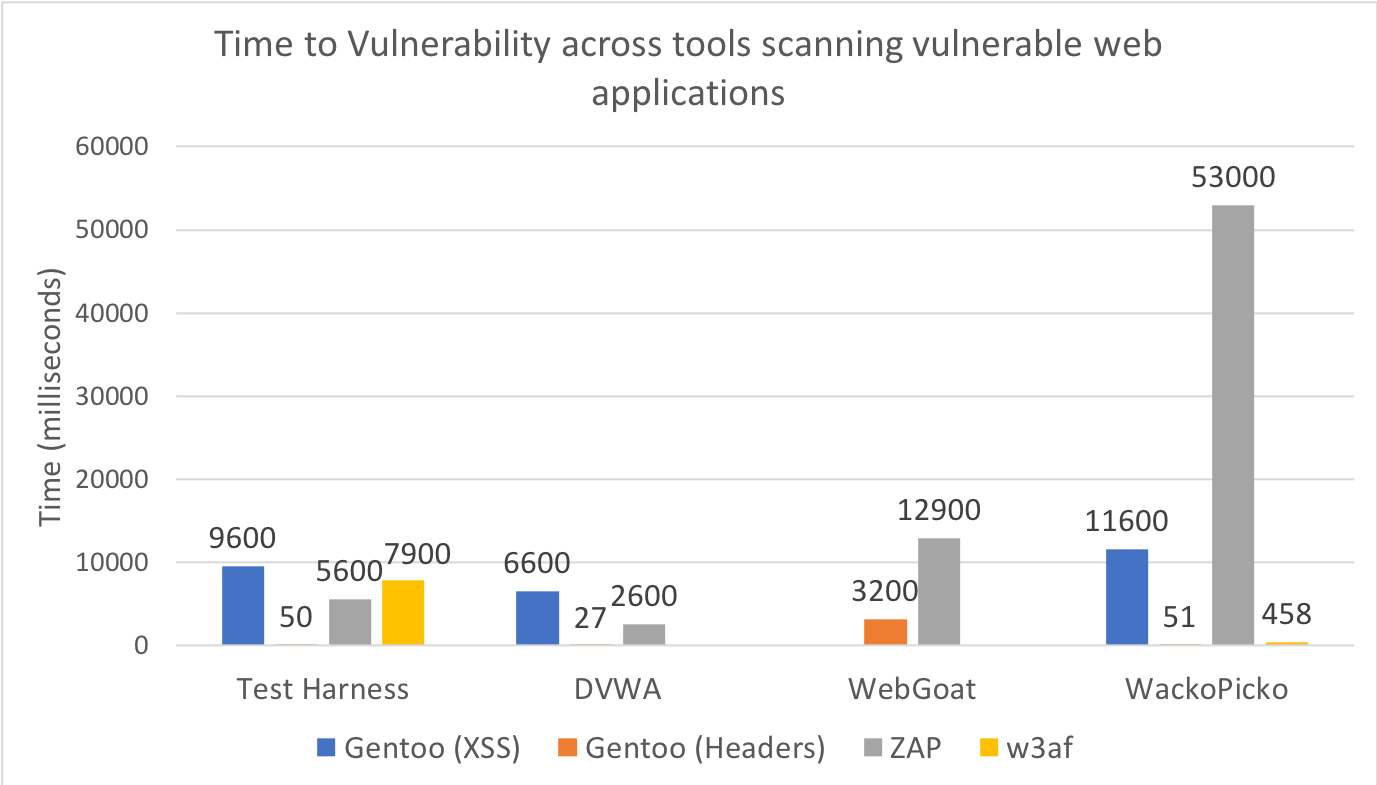
\includegraphics[width=\textwidth]{images/evaluation/time_to_vuln.png}
	\caption{This figure shows the trends across each tool's \textit{Time to Vulnerability} metric}
	\label{fig:time_to_vuln}
\end{figure}

We argue that the numbers presented in Figure \ref{fig:time_to_vuln} are qualified to be compared as-is. An argument could be made that these numbers are biased towards Gentoo because the extension is only looking for one type of vulnerability on each scan, whereas ZAP and w3af have to scour the entire application for vulnerabilities. However, it is that very broad scope which ZAP and w3af have access to which counter-balances the argument - both of these tools can search for \textbf{any} possible vulnerability in whichever order they please. This means they can report easier to find vulnerabilities more promptly than Gentoo. That is what we observed with w3af - this tool produces alerts and warnings for some more esoteric vulnerabilities than ZAP and Gentoo, which contributes to its accelerated pace in reporting vulnerabilities (especially notable in the WackoPicko scan). ZAP does not seem to perform as homogeneously as the other tools, but it certainly makes up for this in its consistency and range of vulnerability detections, as shown in the alert figures above. \\

It is pleasing to see that Gentoo has a consistent performance in raw speed of finding a vulnerability from the start of the scan, and that the wait for a specific vulnerability identification is in line with expectations of its user interaction (slower than automatic) and the complexity of the web application. This trend is seen both in the XSS and in the Passive Header scans. \\

We now analyse the \textit{Interaction Volume} for each of the tools, and produce a comparison between these. \\

\begin{figure}[h]
	\centering
	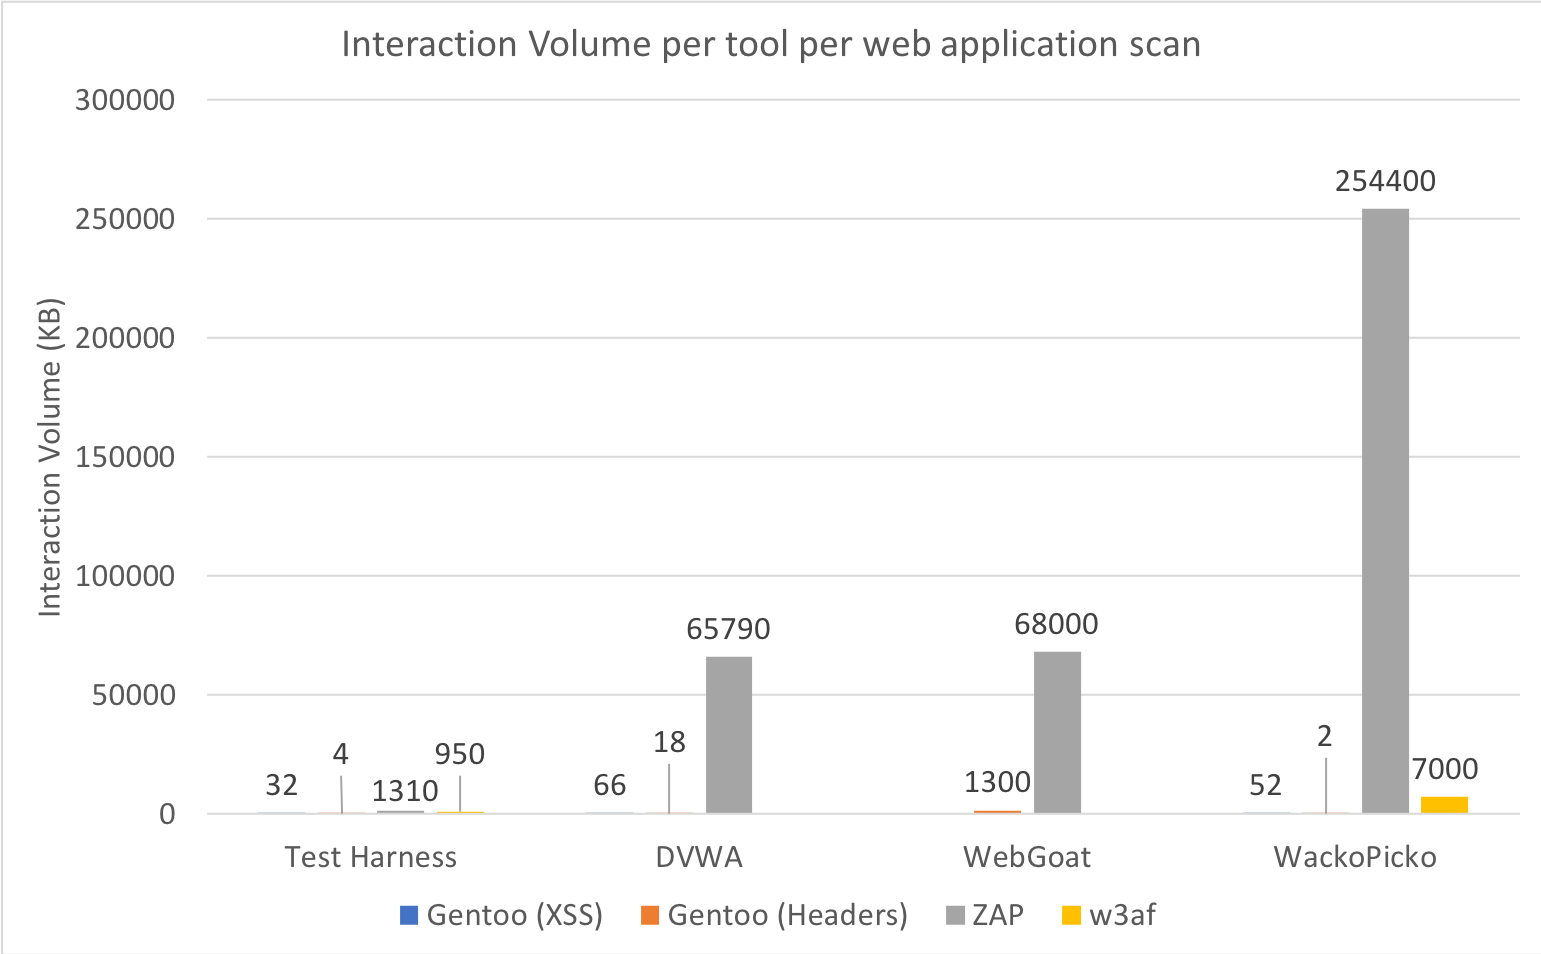
\includegraphics[width=\textwidth]{images/evaluation/interaction_to_volume.png}
	\caption{This figure shows the trends across each tool's \textit{Interaction Volume} metric}
	\label{fig:interaction_volume}
\end{figure}

It is abundantly clear from Figure \ref{fig:interaction_volume} that ZAP has an overwhelmingly larger amount of data transferred in its scans than any of the other tools. In comparison to the others, Gentoo has a consistently small interaction volume in every scan. Unlike the \textit{Time to Vulnerability} metric, the \textit{Interaction Volume} measure is far more dependent on the scanner's scope of attack - the more vulnerabilities a scanner targets, the more requests will have to be sent out (potentially fuzzed) to trigger a wider range of vulnerabilities. As the web application complexity grows, the \textit{Interaction Volume} figures of full-scan tools inflate alongside it, whereas scanning for 1 vulnerability involves attempting the same attack on whatever the surface area presented to attack might be. Therefore, it is reasonable to suggest a normalisation factor for a more apt tool comparison. For the outputs of ZAP and w3af, we divide the \textit{Interaction Volume} by the confirmed number of dangerous vulnerabilities found by each scan to give us the \textit{Normalised Interaction Volume}. This normalised metric should give us a comparison metric that is correlated to the success of the tool - the better it performs in finding vulnerabilities, the lower the \textit{Normalised Interaction Volume}.\\

\begin{figure}[h!]
	\centering
	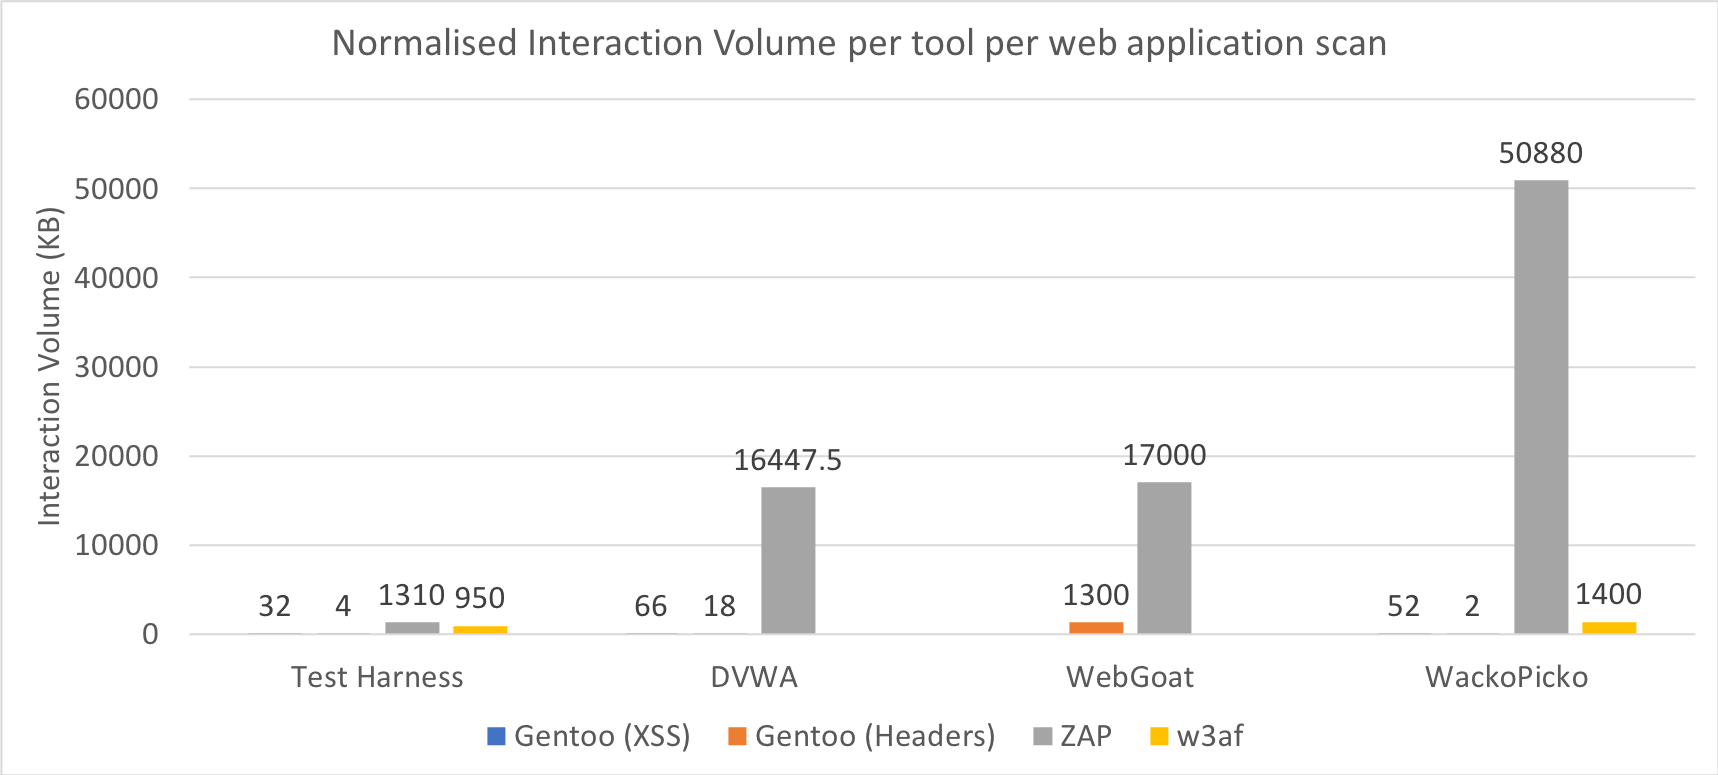
\includegraphics[width=\textwidth]{images/evaluation/normalised_interaction_volume.png}
	\caption{The \textit{Normalised Interaction Volume} mostly affected the figures for ZAP, giving it a fairer means of comparison against Gentoo and w3af}
	\label{fig:normalised_interaction_volume}
\end{figure}

As shown by Figure \ref{fig:normalised_interaction_volume}, the largest change between the \textit{Interaction Volume} and the \textit{Normalised Interaction Volume} metrics is the scale by which ZAP shows a much larger \textit{Interaction Volume} than its competitors (the scale has approximately been divided by 5 from Figure \ref{fig:interaction_volume} to Figure \ref{fig:normalised_interaction_volume}). Clearly, despite the normalisation, ZAP still has an overwhelmingly large amount of \textit{Interaction Volume} when compared to Gentoo and w3af. Gentoo dominates in this category, requiring very little page interactions to successfully fingerprint XSS vulnerabilities. \\

 We see that the \textit{Normalised Interaction Volume} for Gentoo's XSS scan scales with more complex web applications, but in a controlled way, such that it remains the best performer in this category. A low \textit{Normalised Interaction Volume} is desirable as the tool is more likely to remain unnoticed for a longer period of time than its competitors. Web application servers that log requests could easily identify tools such as ZAP and block further requests for fear of Denial of Service or other attack. In a similar situation, Gentoo would remain stealthier for a longer period of time, which is a desirable feature for a penetration tester. \\ 

Lastly, we look at the \textit{Number of replays / attacks needed} (to get to the first vulnerability) for each of the produced scans. As Figure \ref{fig:number_replays_first_vuln} shows, once again, the figures for this metric are heavily skewed when looking at the outputs from ZAP. While Gentoo performs particularly well in this category (with the largest number of replays for any of the scans barely hitting double digits), we can also see that w3af performs reasonably well. \\

\begin{figure}[h!]
	\centering
	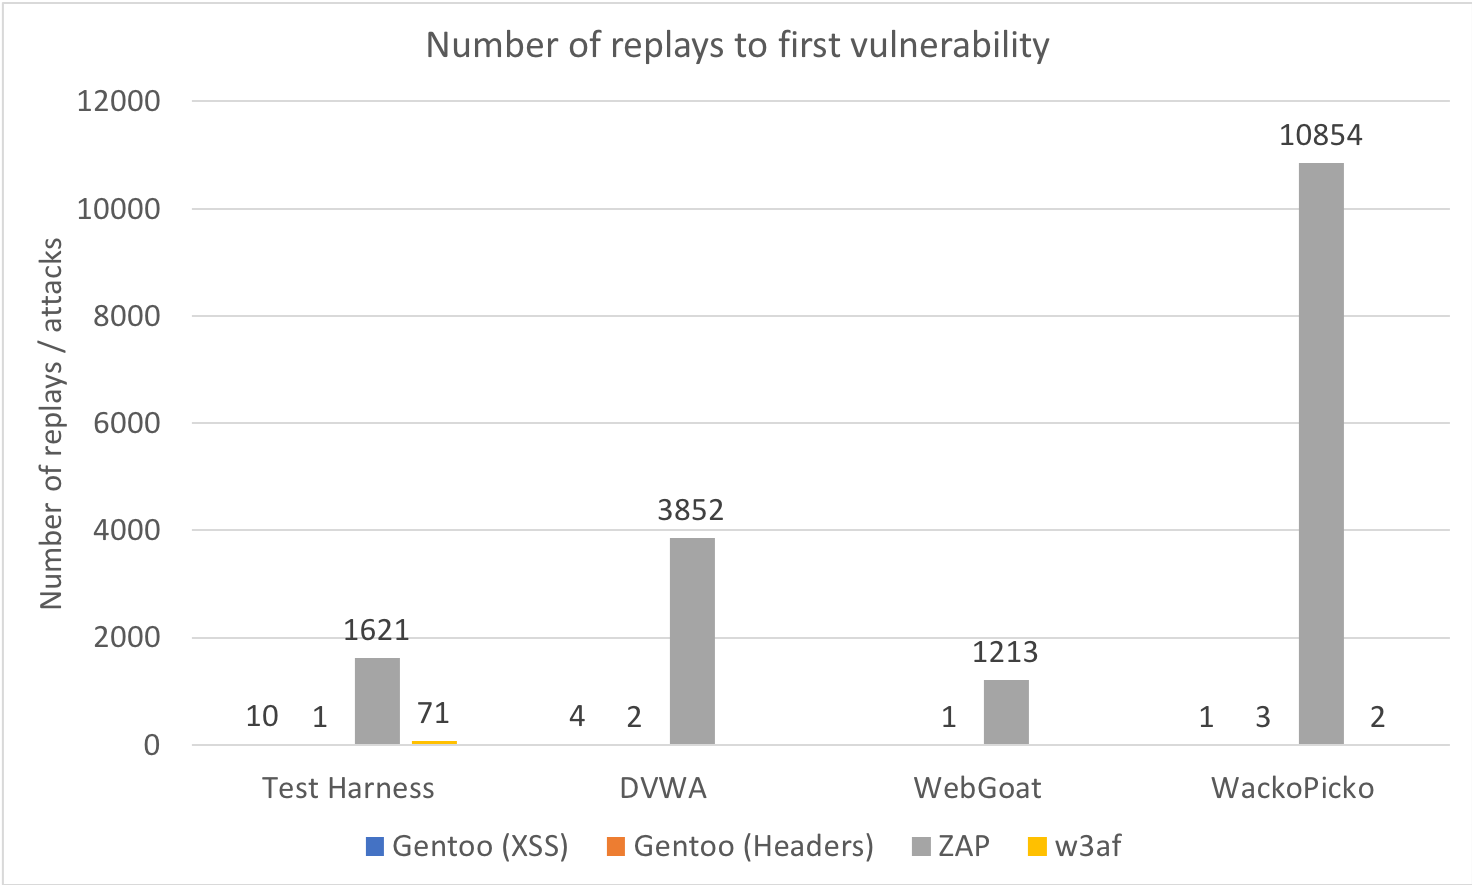
\includegraphics[width=\textwidth]{images/evaluation/number_replays_first_vuln.png}
	\caption{The number of attacks or replays required in a scan to reach the first diagnosed vulnerability}
	\label{fig:number_replays_first_vuln}
\end{figure}


 Clearly, with more requests this metric is easily dilated or distorted - as we have seen from the previous data points, ZAP sends out a far larger number of requests than Gentoo or w3af. Thus we prepare this statistic from a different perspective, the percentage of the scan at which the first vulnerability was found (or \textit{Scan completion to first vulnerability}). Instead of measuring how many raw requests are made until a vulnerability is found, it normalizes the data to a percentage of the scan. We see the results in Figure \ref{fig:scan_completion_first_vuln}. \\
 
 \begin{figure}[h!]
 	\centering
 	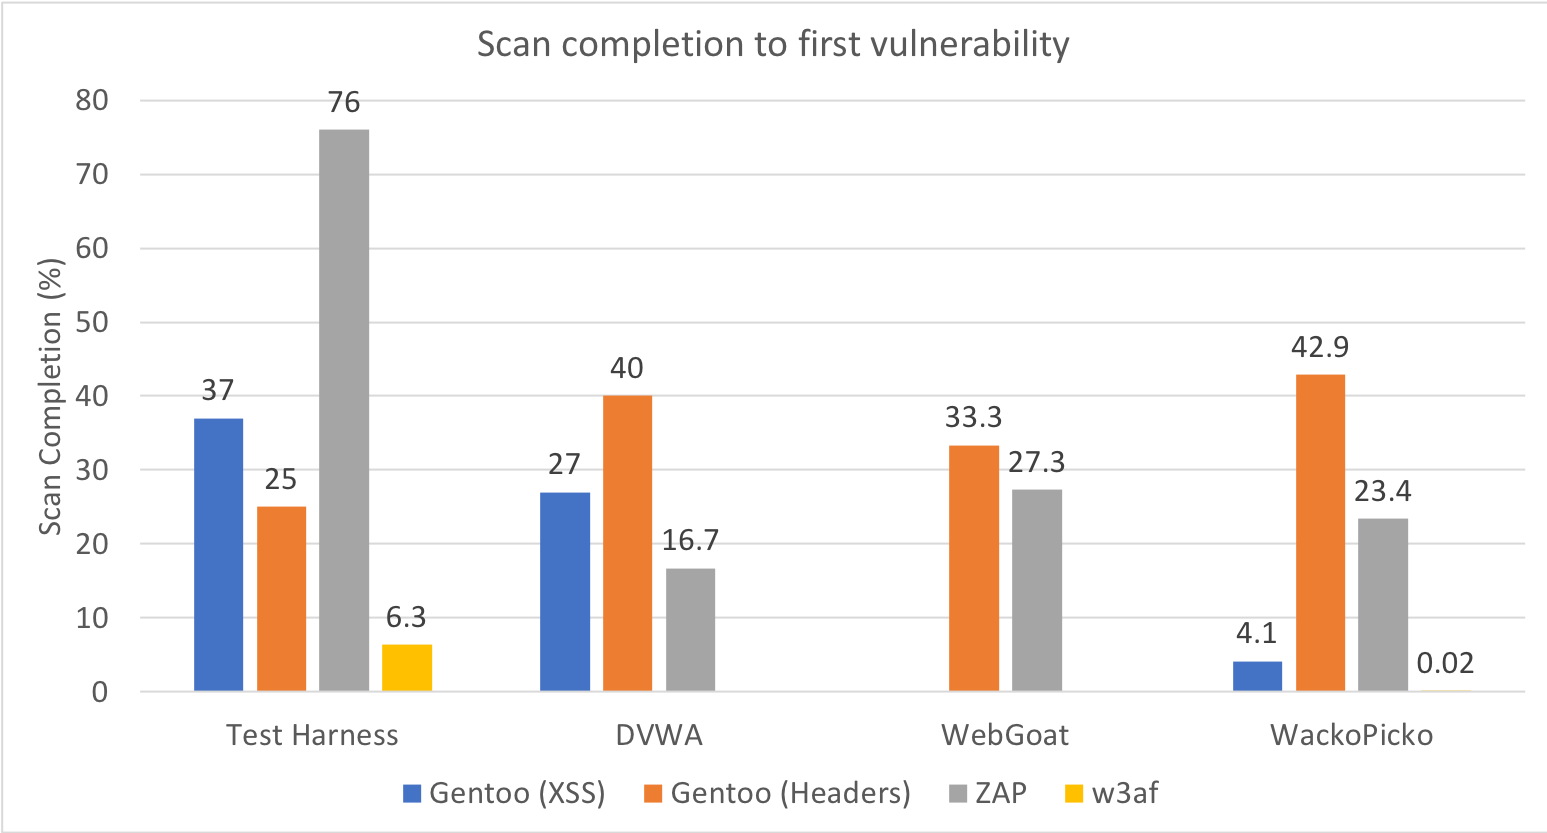
\includegraphics[width=\textwidth]{images/evaluation/scan_completion_first_vuln.png}
 	\caption{The percentage to which the scan was complete when the first vulnerability was found}
 	\label{fig:scan_completion_first_vuln}
 \end{figure}
 
 This metric gives a more interesting basis for analysis. Here, we see that the Gentoo Passive Header scan shows a very stable \textit{scan completion} metric when compared to the other scans. The Gentoo XSS scanner displays positive results here, with all of the \textit{scan completion} results being below 40\%. This leads us to believe that throughout its scans, it detects vulnerabilities with focused attack vectors, making judicious use of its requests. With an even better success rate for this metric, w3af has an extremely low \textit{scan completion} rate, with the worst of the 2 values being under 10\%. This indicates that of the 3 tools, w3af is the best at quickly identifying vulnerabilities, irrespective of their severity. This greedy approach is desirable for pentesters, as this hastily provides them with more information during their \textit{information gathering} phase of testing a web application. \\
 
 Although the \textit{scan completion to first vulnerability} metric provides a more normalized comparison point than the \textit{number of replays / attacks needed to first vulnerability}, it is important to note that it is mathematically skewed to profess superior statistics to scans in which a larger number of requests is sent. In scans with fewer overall requests (namely the Gentoo XSS and Gentoo Headers), each request which is unsuccessful in uncovering a vulnerability counts more towards the \textit{scan completion to first vulnerability} measurement than a similar request for scans which employ more requests overall. In one of the data points (Gentoo Header scan in WebGoat), a total of 3 passive requests were made, of which the first instantly generated an alert which was logged in Gentoo. Despite this seemingly 'perfect' performance for this intended measurement, the \textit{scan completion} metric (correctly) records this at 33\%, which misleads a reader of Figure \ref{fig:scan_completion_first_vuln} into thinking that Gentoo is performing relatively badly. \\
 
 Overall, given the very low numbers reported for the \textit{number of replays / attacks to first vulnerability} as well as the stable numbers for the \textit{scan completion to first vulnerability}, it is fair to deduce that Gentoo has also performed well in this category. This attests that the attacks generated by the extension are executed in a relevant order; attacks that are more likely to uncover vulnerabilities are expected to be ran before other esoteric attacks. \\
 
 In review of the analysis of these metrics between the different tools, we observe the following: 
 
 \begin{itemize}
 	\item ZAP is the most successful of the tools in reporting significant vulnerabilities. This comes at the cost of larger and longer-running scans, which subsequently results in a more conspicuous web application scanner. A large number of requests can more readily identify potential attackers and intruders into an application, which is not desirable for penetration testers (in black-box testing situations).
 	
 	\item w3af produces alerts and warnings for more esoteric vulnerabilities than either ZAP or Gentoo. This tool is also quick to point these out, making it a good option between those analysed for a web analyst in terms of value for time spent.
 	
 	\item Gentoo performed well in all 3 metrics analysed - given that it is only semi-automated, it is still reasonably fast at detecting \textbf{targeted} vulnerabilities. It does so with a small online footprint; we recorded it to have the lowest \textit{normalised interaction volume} of all the tools in the tests. Its attacks are also concise, they quickly detected the intended vulnerabilities as far as the scope of the tests above has shown. The successful performance in these 3 metrics validates the implementation as described in Chapter \ref{implementation}.
 	
 	\item Comparing Gentoo as a human interaction based scanner to fully automated black box scanners is difficult. Different metrics must be analysed in tandem, and we cannot be quick to make absolute judgements on the success or failure of these in comparison to another. 
 \end{itemize}

\section{Live application scanning}

As demonstrated in Section \ref{live_vulnerability}, Gentoo was used as a driving tool behind the uncovering of a real vulnerability on a live website with a significant amount of traffic. The process behind this discovery was very informal - Gentoo's Recommendations feature was often left on after development sessions as we browsed through the internet. We sporadically and (mostly) randomly clicked the recommendations button to see whether Gentoo would be able to uncover any interesting behaviour in websites (at the very least). \\

Indeed, this turned out to be the case. In many websites, triggering Gentoo's Recommendations prompted webpages to produce interesting error pages (some of which revealed relevant information, such as the \texttt{Server} and the \texttt{Powered-By} headers common to many web servers nowadays, as well as versioning information) - in a scenario where a pentester would target these websites, this would be very relevant in the \textit{information gathering} phase. \\

The HTML injection vulnerability detected arose as a result of unexpected behaviour triggered by the recommendations. It was not expected that Gentoo would be used in successfully finding a live vulnerability - this was considered to be an added bonus. The successful identification of this vulnerability thus proved that the implementation of the low effort Recommendations feature was a great success. \\


\section{Accessibility}

Finally, we evaluate different accessibility aspects of the extension. We begin by looking at some compatibility aspects. As we have seen, Gentoo was unable to scan WebGoat due to a scripting error, for reasons we were unable to diagnose. Being incompatible with one of the vulnerable web applications hinders our ability to produce an effective comparison between Gentoo and its competitors. It also highlights what we will call 'creator's bias' - since we have built and tested Gentoo using the Test Harness, the tool becomes overfitted to detecting vulnerabilities in this web application. Thus, when we eventually test the extension against other applications, due to lack of testing or programming generalisation, as seen with WebGoat, the extension is unable to scan for vulnerabilities. This also explains the reason as to why Gentoo was unable to detect the Persisted XSS vulnerability within DVWA. Although the \texttt{textarea} HTML tag is a valid form input, it was not included in the Test Harness. As a result, Gentoo's Action Replay algorithm does not check for additional inputs submitted through \texttt{textarea} - meaning it skips out on detecting an important vulnerability. \\

One of ZAP's most useful features is being able to open a browser window at the URL which is being attacked. While it is open, ZAP logs the user's input, including any credentials used in form submissions, to help with crawling the web application. This feature is not present in w3af, making it very reliant on its own authentication mechanisms. These were difficult and unreliable to setup, meaning w3af was effectively unable to scan both DVWA and WebGoat. In comparison, Gentoo has no need for this feature because it is inherent to how the browser extension functions - the program has direct access to the web application, and effectively acts as a middle-man between it and the user. The user does not need to worry about crawling nor authentication beyond their own account, because Gentoo acts as a companion, analysing whatever website the user decides to browse. Thus Gentoo incorporates one of the most useful features in web app scanners by default, massively improving its usability. \\

As part of development, we have created a user feedback form for interested people who were willing to partake in a small experiment to gather data on how users used Gentoo. Although this experiment has not yet gathered enough data for statistical relevance, some of the user feedback regarding usability is useful to consider. While observing users attempt to uncover the XSS vulnerability using Gentoo on the Test Harness, it became clear that of all the mechanisms in the extension, using the Action Replay mode was particularly unclear. Although there are some limited instructions written in plaintext in the popup page regarding usage, users were still confused about how to use the Action Replay, and made no progress in uncovering vulnerabilities on their own when using this mode. Thus, accessibility for users in Gentoo could have been improved by adding a guided tutorial or a plaintext page with instructions on how to use the extension itself. This also highlighted that Gentoo failed to successfully address the education concerns the project hoped to tackle. The lack of the user guidelines page not only makes it harder for the user to understand how Gentoo works, but also makes no headway in educating the user in generic web vulnerabilities, let alone those the user might exploit whilst using Gentoo.  \\ 







\chapter{Future Work}
\chapter{Conclusion}

We conclude this thesis with some ideas on how to further improve the body of work thus far, and make an overall collection of thoughts on Gentoo. \\

\section{Future work}

It is easy to see how Gentoo could be taken some steps further. One of the first potential additions to this would be to incorporate the scanning for SQL injetions. This particular type of vulnerability would express itself in a very similar way to what has already been shown in the Reflected XSS. The concept of these two vulnerabilities is similar - a malicious input is injected into a form, and the output is analysed in search of clues of injection. In the case of encoding an SQL Injection analyser, this might involve searching the response body for database-like query outputs, or for error pages that slowly leak information such as the version of the database, or react to blind injections (perhaps the page takes longer to load because a successful delay command has been executed as part of the malicious payload). Given the framework we have built up with Gentoo, detecting and preventing SQL injections would be the next logical step to follow in expanding the suite of vulnerabilities Gentoo can detect. \\

Another improvement would be to make more effective use of XMLHttpRequests, particularly in the Action Replay mode. In the current code version, Gentoo will load a new attack window per generated attack - doing so allows the extension to evaluate any Javascript ran as part of a potential attack in the new window, since the evaluated body is not part of the initial request response. Doing so can become extremely cumbersome however, especially if we were to expand the suite of attacks. At the moment, the automatic launch of several new tabs can severely slow down the machine, or in more memory-starved situations, crash Google Chrome altogether. Using XMLHttpRequests would bypass this situation; these requests are performed in the background, and require minimal to no input from the user when compared with new tabs being opened. \\

One of the major improvements in attack power would be to enable attack fuzzing. In the current version of Gentoo, each existing attack payload is hardcoded, and none of the attacks will deviate from this. However, with the vast expanse of the internet, it is very likely that a potential website \texttt{A} suffers from a vulnerability when injected with the specific payload \texttt{P}, whereas website \texttt{B} might suffer from an injection of payload \texttt{P'}. It is not the case however that \texttt{A} is vulnerable to payload \texttt{P'}, or \texttt{B} to \texttt{P}
 for that matter. But what if the only difference between \texttt{P} and \texttt{P'} is a single \texttt{"} character? It is hard to justify the hardcoding of all these possibilities, which is where the power of input fuzzing would come in. Using this, only one base input type would have to be hardcoded, whilst all the other inputs would be automatically generated as per the defined regex rules. Using a fuzzer engine to generate attack payloads would exponentially increase the attack surface area of Gentoo, although care would have to be taken to discerningly choose which regex rules would be selected so as to generate good quality input fuzzes. \\
 
 Gentoo could also be improved from a user centric design overhaul. Specifically, an interactive tutorial that guides each new user in a step by step experience that teaches how to use the different attack modes would be of great use. Such a tutorial would be of particularly great aid to new users coming to grips with how the Action Replay mechanism works, as this mode is complex, and the steps to follow and the order in which to execute them is not immediately clear. Adding this feature alongside a text knowledge base explaining different vulnerabilities and their significance would also address the concern of educational deficiency of Gentoo.  Doing so would also give users another chance to become more educated on how to diagnose vulnerabilities. This would improve usability and create a far more polished end product. \\
 
 This project would also have very likely benefitted from benchmarking Gentoo against a more extensive list of competitors. Both ZAP and w3af are open source web application scanners, so we did not ascertain how Gentoo would have performed when set side by side against commercial tools. This leaves a gap for further investigation in the project. \\



\section{Final Remarks}


This project has ambitiously saddled on the margin of automation when it comes to black box web application scanners. Gentoo finds itself as a hybrid tool that automates the bulk of work, but only when it is told to by a user. We think that this hybrid approach is one worth exploring further, especially because certain vulnerability diagnosis and exploitation is a complex task, which is likely to require human validation for a while still. \\

We saw how this automation can be useful in a low effort scenario using the Recommendations, how it was used in active user-led scans by using the Action Replay mechanism, and how it can be leveraged in its entirity for Passive scans. Each of these modes has their own perks and separate advantages. We were particularly content to see the validation of the hypothesis that vulnerability diagnosis and exploit is a delicate process by uncovering the live vulnerability; although this was triggered through use of the Recommendations feature, it was only fully exploited afterwards using trial and error. Doing so legitimized much of the work being done on this project. \\

We think this project explored through its analysis that there is no right or wrong approach in whether a scanner is fully automated or perhaps semi automated, as there are good and valid arguments both for and against each of these variations. Through numerical analysis of the two types, we came to the conclusion that Gentoo's implementation was successful in delivering a focused, lightweight scan, which successfully met some of the key metrics we were hoping to observe from such a tool. Perhaps more importantly here is ascertaining that the abstraction of using a browser extension was particularly advantageous from a user's perspective because the extension leverages its power and granted permissions to co-exist very closely between the user and the application under test. \\

 This takes us back to the initial project proposal - is it possible to design a browser extension which passively analyses the web traffic the user makes and reports it back if signs of a web vulnerability have been detected? Given the analysis performed, and the real-life experience under its belt in such a short period, it's fair to say that Gentoo met most of the project criterion. Although it underperformed in its educational aspect, it effectively leveraged its position as an extension to be able to meet the remaining project goals. Gentoo shows that a scanner working as an aide to a human penetration tester is powerful and fit for purpose.
 





































\appendix
\chapter{First Appendix}

\bibliographystyle{plain}
\bibliography{bibs/sample.bib}

\end{document}